\def\q{\mathbf{q}}
\def\dq{\mathbf{\dot{q}}}
\def\J{\mathbf{J}}
\def\A{\mathbf{A}}
\def\B{\mathcal{B}}
\def\C{\mathcal{C}}
\def\T{\mathcal{T}}
\def\W{\mathbf{W}}
\def\b{\mathbf{b}}
\def\I{\mathbf{I}}
\def\x{\mathbf{x}}
\def\dx{\mathbf{\dot{x}}}
\def\e{\mathbf{e}}
\def\de{\mathbf{\dot{e}}}
\def\w{\mathbf{w}}

\externaldocument{architecture}

\todo{ADD material from the original ICRA work}
The field of whole-body planning and control tries to find the solution to the problem of executing one or more task at the same time, while exploiting the capabilities of the entire body of redundant, floating-based robots in multi-contact scenarios with the environment.

%The problem entails modeling and controlling systems with hybrid dynamics, encompasses the force distribution problem in multi-contact scenarios, planning for the making and breaking of robot-environment contacts during loco-manipulation tasks, and passes through the optimization of the robot resources to maximally exploit the kinematic structure and the dynamics of the robot and the task.
%Related problems to the whole-body control are of mechatronic(how to design an agile and robust robot), and computational origin: the joint design (compliant, rigid), as well as the search for designs to obtain reliable low-level torque control, and in the case of compliant joints, performant low-level position controls, and under the computation point of view, fast numerical methods, software and hardware architectures able to accomplish high frequency, reliable control.
%Other than being a research problem, it still is a technological problem to either implement, simulate and control highly redundant robots, such as humanoid robots. Not only the prices for building such robots are still very high, being the assembly of robots ironically man-made (with a very interesting and ambitious vision from Boston Dynamics to 3d-print the robots of the future), but the technological problems range from the problem of building a reliable, high-throughput and high-bandwidth communication network between the sensors, actuators and controllers, to obtaining reliable torque sensing at the joint level, to building agile robots which are also resilient, and of course to the computational limitations one encounters when writing control algorithms for highly redundant robots.

Several and different approaches are being investigated by the research community, such as optimization, inverse dynamics, inverse kinematics with dynamic filters and admittance control. \todo{how long is this so far? I could also go in more detail on the state of the art of several kind of control? Or briefly on the problem in general, and more in detail on the kinematic problem}.

Inverse Kinematics (IK) is a fundamental component for a vast number of application in robotics. In particular, kinematic control is still a popular choice for high level robot controllers. While the kinematic control problem has been tackled in literature using several different approaches, latest trends both in research and application make use of Quadratic Programming (QP) to obtain a locally optimal solution to the hierarchical constrained IK problem. The interest is in part justified by the need, for practical reasons, to have robust solutions which are hard constrained by the physical limits of the robots, such as joint, torque and self-collision avoidance limits. In this section the theoretical foundations of kinematic control based on QP optimization will be presented, and the formulation of a comprehensive set of tasks and constraints will be provided, according to the capabilities of the developed framework. The kinematic control, and thus the formulation for the tasks and the contraints in the framework will be expressed at the velocity level, meaning the solution of each step of the IK solver will return a displacement $\delta q$ that can be actuated on the physical robot or integrated for kinematic simulation. Some aspects of the IK solver will be described, and the choice of the state-of-art QP solver library \emph{qpOASES} will be motivated. 
The work presented has been been developed as part of the robotic framework \textbf{OpenSoT}, developed at the Italian Institute of Technology \cite{Rocchi2015-is, Fang2015-cr, Ajoudani2014-fs, Lee2014-dg}. The framework has been developed for application to our compliant humanoid robots, in particular to the COMAN in a compliant inverse kinematics scheme, and WALKMAN as part of the high-level control architecture  used in the Darpa Robotics Challenge. The framework consists of a C++ library tailored for the control of hyper-redundant fixed/floating base robot. Experiments and results in the Darpa Robotics Challenge are presented later on in this section, while the software API and tools as will be presented in chapter \ref{architecture}.

%%%%%%%%%%%%%%%%%% INTRO
\section{OpenSoT: a library for Whole-Body Control of Humanoid Robots}
\begin{wrapfigure}{r}{0.35\textwidth}
  \begin{center}
    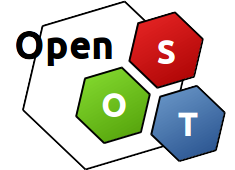
\includegraphics[width=0.25\textwidth]{images/openSoT_stickers}
  \end{center}
  \caption{OpenSoT Logo}
\end{wrapfigure}
From a very broad perspective, the inverse kinematics problem is that of mapping task-space objectives into joint-space commands.
Typical techniques to map task-space commands to joint commands can be roughly classified as inverse kinematics or inverse dynamics schemes and can be implemented using a variety of low level controllers.
\textbf{OpenSoT} is a novel whole body motion library developed at the Italian Institute of Technology (IIT), which belongs to the former group: our goal has been to develop a high performance and flexible library that can generate reliably complex and efficient whole body motions.

The \emph{Differential Inverse Kinematics Problem} consists of the determination of the joint trajectories corresponding to a given task for the end-effector in \emph{Operational Space}. This problem is in general highly non-linear, a \emph{closed form} solution may not be available, and may have multiple solutions. In the case in which the robot is \emph{redundant} with respect to the task, that is, the degrees of freedom of the robot are greater than the degrees of freedom required by the specified task,  the IK Problem admits an infinite number of solutions. In case of operational space control, at least a solution is guaranteed to exist if the given goal in operational space belongs to the manipulator \emph{dexterous space}.
Despite the relationship between joint position variables and operational space poses is not linear, the mapping between joint velocity variables and operational space velocities is linear through the robot Jacobian:
\begin{equation}
    \label{eq:differential_kinematics}
    \dx = \J(\q)\dq
\end{equation}
where the Jacobian $\J$ (we will skip the dependency on the actual configuration $\q$ from now on) is expressed from a certain \emph{base link} to a certain \emph{distal link}, and operational space velocities $\dx$ of the \emph{distal link} are expressed in the \emph{base link} reference frame\todo{can be written more clearly. The Jacobian depends on three dimensions, the location of the pole, the location of the frame of reference, and the orientation of the frame of reference. See from the KDL documentation :)}.
A general solution, for the redundant case, of (\ref{eq:differential_kinematics}) is:
\begin{equation}
    \label{eq:differential_inverse_kineamtics}
    \dq_\text{d} = \J^{\dagger}\dx_\text{d} + \left( \I - \J^{\dagger}\J \right)\dq_\text{0}
\end{equation}
where $\J^{\dagger}$ is the \emph{pseudo inverse} of the Jacobian and $\dq_\text{0}$ is an arbitrary joint space velocity. 
This solution allows also for \emph{task prioritization}: 
\begin{equation}
    \label{eq:another_task}
\dq_\text{0} = \J_\text{0}^{\dagger}\dx_\text{0}
\end{equation}
in particular, the solution given by (\ref{eq:differential_inverse_kineamtics}) with (\ref{eq:another_task}), projects the joint velocities of the second task into the null space of the first task removing all the components that would interfere with it \cite{DBLPReferenceRobo2008}. Many other solutions of (\ref{eq:differential_kinematics}) are available in literature \cite{siciliano1991general}. \todo{put solution by Siciliano}. Singularities in the Jacobian, as well as joint velocity limits, are often handled with the \emph{Singularity Robust Inverse} (SRI) \cite{nakamura1990-tp}, \cite{maciejewski1989-jp}.
The problem of this type of schemes is that they do not handle constraints in the form of inequalities. 

To overcome this problem, techniques from the optimization field have been adopted.
We can consider the inverse problem of (\ref{eq:differential_kinematics}) as a Quadratic Programming (QP) problem with linear constraints:
\begin{equation} 
\label{eq:optimization_problem}
\begin{array}{c}
\dq_\text{d} = \underset{\dq}{\operatorname{argmin}} \ \Arrowvert \J \dq-\dx_\text{d} \Arrowvert\\
s.t. \ \mathbf{A}\dq \leq \mathbf{b}
\end{array}
\end{equation}
%where $\Arrowvert \J \dot{\q}-\mathbf{v}_d \Arrowvert = \dot{\q}^\text{T}\J^\text{T}\mathbf{J}\dot{\q} - 2(\J\dot{\q})^\text{T}\mathbf{v}_d+\mathbf{v}_d'\mathbf{v}_d$ is the quadratic cost function that is minimized and $\mathbf{A}\dot{\q} \leq \mathbf{b}$ is a general linear constraint. 
The two most popular families of methods to solve the problem in (\ref{eq:optimization_problem}) are \emph{active set} and \emph{interior point} methods. 
\emph{Active set} methods consider constraints as equalities, in the circumstance when they are active, so that the problem (\ref{eq:optimization_problem}) is transformed in a QP with only equalities. At each iteration the new active set is computed checking for the infeasible constraints.
\emph{Interior point} methods use barrier functions (such as $log$ functions) to penalize the cost function in the region where the bounds are violated and the solution is found by iteratively relaxing the barrier function\todo{it should be the opposite?}.
Even under the optimization point of view, the task prioritization can be handled considering the minimization of the cost function under equality constraints given by the minimization of previous tasks. This technique is commonly referred as \emph{Stack of Tasks} (SoT) \cite{mansard:icar:09}. 

\textbf{OpenSoT} implements the idea of decoupling atomic tasks/constraints descriptions and solvers to execute multiple tasks and achieve complex motion behaviors. It employs a solver implementing a cascade of QP problems, and a set of tasks and constraints in velocity space in order to solve a generic hierarchical inverse kinematics problem on a floating or fixed base robot. The stock IK solver consists on a state machine that hides all the complexity of the underneath QP solver based on a state-of-art library in QP resolution using the active set approach: \emph{qpOASES} \cite{ferreau2013}.
This yields the following features that make the implementation of \textbf{OpenSoT} unique and attractive:   
\begin{itemize}
\item Demonstrates adequate modularity through the separation of task descriptions, control schemes and solvers maximizing customization, flexibility and expandability.  
\item Provides user friendly interfaces for defining tasks, constraints and solvers to promote integration and cooperation in the emerging field of whole-body hierarchical control schemes.
\item Demonstrates computation efficiency to allow for real time performance implementations.
\item Allows ease of use and application with arbitrary robots through the Universal and Semantic Robotic Description Formats (URDF and SRDF).
\end{itemize}
The reliability and robustness of \textbf{OpenSoT} framework has been proved during the DRC Finals since it has been used by the WALK-MAN team, to perform all the manipulation tasks involving \emph{whole-body} motions while taking into account various type of constraints. During the development period, the \textbf{OpenSoT} framework allowed the fast evaluation of different formulations of the whole-boby control problem in order to optimally solve the tasks of the competition, thusly demonstrating the benefits of a flexible high-level framework in robotics rapid application development. 
The architecture of \textbf{OpenSoT} encourages collaboration and helps integration and code maintenance.

%\todo{should I integrate some of this stuff here?}
%Recent approaches make use of Quadratic Programming (QP) Optimization that makes also possible to specify linear constraints for the IK to affect the solution:
%\begin{equation}
%\begin{array} {ccc}
%    \dq_d  = & \underset{ \dq }{ \text{argmin} } & \left\| \J_n \dq - \dx_\text{n,d} \right\| + \lambda \left\| \dq \right\| \\
%    & {s.t.} & \A_1 \dq = \A_1 \dq_1 \\
%    & &  \vdots \\
%    & & \A_{n-1} \dq = \A_{n-1} \dq_{n-1} \\
%    & & \A_{c,1}\dq \leq \b_{c,1} \\
%    & & \vdots \\
%    & & \A_{c,n}\dq \leq \b_{c,n}
%\end{array}
%\label{eq:sot_full}
%\end{equation}
%where $\A$ matrices and $\b$ vectors are constraints.
%In \eqref{eq:sot_full}, priorities are taken into account considering the previous solutions $\dq_i, \; i < n$ and constraints of the type {$\mathbf{A}_i \dq = \mathbf{A}_i \dq_i, \; \forall i < n$},  so that the optimality of all higher priority tasks is not changed by the current solution \cite{mansard:icar:09}. The second term in the cost function of \eqref{eq:sot_full} permits to handle kinematics singularities in order to avoid high joint velocities \cite{nakamura1990-tp}. A similar structure can be used to solve the IK problem at the acceleration level.

%Many tasks and constraints have been presented in literature for the framework depicted in \eqref{eq:sot_full}, examples are: joint limits, joint velocity limits, self collision avoidance \cite{kanehiro2008local}, Cartesian velocity limits, minimum joint acceleration \cite{flacco2012-cr} and \emph{Capture Point} \cite{ ramos-humanoid-14} for humanoid robots. In particular, joint limits and joint velocity limits are fundamental when working with real robotic hardware.  

\subsection{Related Work}
\label{sec:related_work_opensot}
Many approaches to solve the IK problem are presented in the literature and most of them address the singularity problem through Tikanov regularisation, with approaches similar to the \emph{Singularity Robust Inverse} (SRI), but lack the possibility to specify constraints, whereas the aforementioned QP formulation allows for an elegant formulation of the IK problem considering linear constraints\todo{write this more clearly?}.
\textbf{OpenSoT} is thus inspired by the \emph{Stack of Tasks}, where the stock IK solver is based on QP (Quadratic Programming) optimization with the possibility to specify \emph{hard} \cite{kanoun2009prioritizing} and \emph{soft} \cite{chiacchio1991closed} priorities between tasks as well as linear constraints and bounds \cite{escande2014hierarchical}.

An interesting approach to hierarchical inverse kinematics resolution is given by \cite{Liu2015-yq} in the form of a Generalized Hierarchical Control (GHC). GHC is developed by means of a novel Generalized Projector which allows to project lower priority tasks into higher priority tasks fully or partially, thus implementing mixable \emph{strict} and \emph{non-strict hierarchies} (i.e. \emph{hard} and \emph{soft priorities}) using a single generalized projecting operation. This allows to mix strict and non-strict hierarchies and to smoothly change priorities, smoothly insert and remove tasks, as well as define complex priority relationships which are better described as a priority network rather than a lexicographic hierarchy.

In \cite{Hauser2014-sq} a method to optimize precomputed joint trajectories so as to satisfy contact and dynamic constraints is proposed.

In \cite{Del_Prete2014-ph} a way to specify hierarchical optimal problems is presented, with application to control of a humanoid robot.

A recent interesting approach is presented in \cite{flacco14revprio}, where redundancy is resolved starting from the lowest priority task.

In \cite{De_Schutter2007-to,Decre2009-om,Decre2013-yt,Smits2009-nv,Vanthienen2012-ed,Vanthienen2013-pl} the \emph{iTaSC} framework is developed, which aims at providing a complete solution for specifying tasks and constraints in a generalized way and provide solvers to automatically compute the control law starting from the task specification. The framework includes also a Domain Specific Language (\emph{DSL}) for rapid application development and formal validation. The method allows for different low-level solvers, and at the moment implements a weighted damped-least-squares pseudoinverse-based (\emph{WDSL-psudoinverse}) velocity control. To the authors knowledge, it has never been tested on humanoid robots.

In \cite{Aertbelien2014-iv} a task specification and solver is implemented using expression graphs, in a similar way (conceptually) to the Stack of Tasks.

In \cite{Pattacini2010-gr} a nonlinear optimization is also performed to perform IK on the iCub platform, where the focus is on Cartesian control of the end-effectors.

There are many other frameworks including those that are based on Inverse Dynamics, implemented on top of a pure low level torque control (a notable example is \cite{Sentis2010-bq}), yet it is difficult to find hardware platforms mature enough to implement control schemes of such frameworks and up to now no complex tasks have been experimentally demonstrated yet in humanoid bipedal robots.
Based on the operational space formalism the \emph{Standard Control Library} \cite{Menon_undated-hv} implements the whole-body multi-task control framework previously cited and it is an updated version of \cite{Philippsen2011-mq}.
A recent new library based on the same concept is \cite{Fok2015-cn}. 

% TODO: cite trak-ik more in depth
In \cite{Beeson15} their solution is compared to popular IK schemes as offered by \emph{KDL} \cite{Smits2011-db}, highlighting the advantages of optimization approaches to the common classic IK schemes.

None of the considered libraries provides a complete set of implemented tasks, constraints and solvers that permits to describes and solve IK problems in an easy and versatile way.
% TODO: Flacco published two interesting papers, "Unilateral constraints in the Reverse Priority redundancy resolution method" (PDF already available, IROS15) and "A Reverse Priority Approach to Smooth Task Transitions" submitted in T-RO, remember to cite as soon as it gets accepted

\subsection{A Framework for Whole-Body Control}
\subsubsection{Whole body control}
\label{sec:walkman_wholebody}
Whole-body control here will be referred to those control laws that allow to execute tasks by using the whole robot structure. The whole-body control laws typically allow to execute several tasks at the same time when possible,  by making use of the redundancies provided by the robot. Preferably they should be as generic as possible in allowing specification of tasks both in Operational and Cartesian space, and in particular, allow for the control in Operational space of any part of the robot, even when does do not coincide with the end-effectors. The whole-body control  problem can be solved by many approaches, as shown in the previous section, but we will concentrate on a kinematic control law that allows to solve the whole-body control problem  in generic kinematic trees, with particular emphasis to the generic case of a floating-base robot.

\subsubsection{Inverse Kinematics}
We consider a robot executing $n$ tasks simultaneously, and for each of these tasks $T_i$, a proper error function $\e_i(\q,t)$ is provided, describing the task error.
The time derivative of the error can be computed as
\begin{equation}
\de_i = \frac{\partial \e_i}{\partial \q}\dq + \frac{\partial \e_i}{\partial t} = \J_i\dq + \frac{\partial \e_i}{\partial t}
\end{equation} 
with $\J_i$ the error Jacobian. During the execution of a generic task it is desirable that the task error converges to 0, by imposing an exponential dynamic, that is
\begin{equation}
\de_i= - \lambda \e_i \Rightarrow \J_i\dq = -\frac{\partial \e_i}{\partial t} - \lambda \e_i = \de^*_i
\end{equation}
If the robot is redundant with respect to a task, secondary tasks can be also added and executed without affecting the performance of the primary task, and given a set of tasks described by the couple 
$T_i = (\J_i, \de^*_i)$, the robot can be commanded to execute them using its whole body motion capabilities. In order to implement the method and obtain this result, the relative importance between tasks needs first to be defined. Thus, two kinds of relationships: \emph{hard priority} and \emph{soft priority} needs to be set. 
A task has a higher \emph{hard priority} with respect to another task if the latter can not deteriorate the performance of the first one. \emph{Soft priorities} are defined between tasks so all the solutions are influenced by each other proportionally to theirs weights, or in other terms, a tradeoff between the performance of competing task is obtained which is continuously tunable by means of a weight coefficient.

The execution of a hierachy of tasks related by an hard priority relation has a well-known solution in the stack of tasks, where hard priorities are enforced by the order of the task in the stack. To take into account also soft priorities the augmented Jacobian formulation \cite{chiacchio1991closed} can be employed. It must be noted though that the augmented Jacobian formulation alone cannot enforce hard priorities since adding many tasks together can generate an ill-conditioned augmented Jacobian matrix.
Therefore, to generate whole-body motions, a series of QP problems in cascade is instead solved \cite{kanoun2011kinematic}. This is a well known method to derive motions by executing tasks adding bilateral constrains to the inverse kinematics problem \cite{escande2014hierarchical}.
A generic task can be described as
\begin{equation}
\begin{array}{ccc}
\dq_i 
   =& \underset{ \dq }{ \text{argmin} } & \left\| \J_i \dq - \de^*_i \right\|\\
         & {s.t.} & \A_{c,1}\dq \leq \b_{c,i} 
\end{array}
\label{eq:Task_1}
\end{equation}
The formulation used in \eqref{eq:Task_1} for the constraints can be profitably used to express lower and upper bounds for the variable value as well as equality constraints.

%According to the classical stack of task method based on null-space projection \cite{sciavicco1988solution} the tasks which needs to be projected in the null-space of the previous task (hard priority) can be generalized in recursive form as:
%\begin{eqnarray}
%\dot{q}_0 & = & 0 \\
%\dot{q}_k & = & \dot{q}_{k-1} + \left(J_kP_{k-1}\right)^+ \left(\dot{x}_k-J_k\dot{q}_{k-1}\right)
%\end{eqnarray}
%where $P_{k-1} = (I - J_{k-1}^\#J_{k-1})$ is the projector
%This is equivalent to the formulation of a stack of optimization problems, with the additional benefit of having explicit unilateral and bilateral constraints. 
In general, the  $n^{\text{th}}$ task will then be written as
\begin{equation}
\begin{array} {ccc}
    \dq_d  = & \underset{ \dq }{ \text{argmin} } & \left\| \J_n \dq + \lambda \e_n + \frac{\partial \e_n}{\partial t} \right\| \\
    & {s.t.} & \A_1 \dq = \A_1 \dq_1 \\
    & &  \vdots \\
    & & \A_{n-1} \dq = \A_{n-1} \dq_{n-1} \\
    & & \A_{c,1}\dq \leq \b_{c,1} \\
    & & \vdots \\
    & & \A_{c,n}\dq \leq \b_{c,n}
\end{array}
\label{eq:sot_full}
\end{equation}
where $\dq_d$ is the joint displacement (control variable) which minimizes the objective function and satisfy the given constraints, if they are a feasible set.
In \eqref{eq:sot_full} the previous solutions $\dq_i, \; i < n$ are taken into account by specifying constraints of the type {$\mathbf{A}_i \dq = \mathbf{A}_i \dq_i, \; \forall i < n$},  so that the optimality of all higher priority tasks is not changed by the solving for the $n$-th task.
%\color{red}
%The minimization of the $W$-weighted $2$-norm of the $n$th task, expressed as before, can be easily transformed into a QP task by writing
%\begin{equation}
%\begin{array} {ccc}
%    \underset{ \dot{q} }{ \text{argmin} } & \frac{1}{2} \dot{q}^T J_{n}^T W J_{n} \dot{q} -\lambda \dot{q}^T J_n^T W \dot{e}^*_n \\
%   {s.t.} & A_{c,n}\dot{q} \leq \text{b}_{c,n}
%\end{array}
%\label{eq:sot}
%\end{equation}
%\color{black}
While in \eqref{eq:sot_full} the first task has a relationship of hard priority with respect to the second, and so on, for each \emph{level} of priority, a soft priority relationship between tasks can be imposed introducing the relative weights $\beta_i$, so that the augmented Jacobians and the error vectors can be written as
\begin{equation}
\label{eq:augmented_jacobian}
\begin{array}{l}
\J_\text{aug}  =  \begin{bmatrix}
\beta_1\J_1^T & \dotsc& \beta_n\J_n^T\end{bmatrix}^T \\ 
\\
\e_\text{aug}  =  \begin{bmatrix}
\beta_1\e_1^T & \dotsc& \beta_n\e_n^T\end{bmatrix}^T 
\end{array}
\end{equation}
where the soft priority between tasks is altered by tuning the relative weights $\beta_i$, with higher priority tasks having larger $\beta_i$. As already mentioned, in this case the tasks can still influence each other's performance.
 A mixture of hard and soft priorities is in general needed to describe a stack of tasks.
 The solution obtained can then be commanded directly to a velocity controlled robot or integrated to command a position controlled robot as
\begin{equation}
    \q_d = \q + \dq \Delta t
\end{equation}
\todo{$\q+\dq$}
where $\Delta t$ is the control loop period.

\subsubsection{OpenSoT} \label{open_sot}
\textbf{OpenSoT} is a robotics library tool oriented to Whole-Body Control. The main idea behind its implementation is to decouple the task and constraint description to the solver used to solve the general Inverse Kinematics/Dynamics problem. \textbf{OpenSoT} aims at providing a standard way to describe the aforementioned entities in an atomic way, and at the same time to build a repository of common entities that can be reused to create a generic stack using a user friendly development and integration interface.

\textbf{OpenSoT} offers classes %(in Fig. \ref{open_sot_inherit})% 
to describe different tasks and constraints whicah can be used to design the robot behavior during the task execution, and solvers with various capabilities and strategies to obtain solutions to the control problem. According to the control type, different controllers are available in literature. Defining a task once in a proper way allows to switch between different control laws, as shown in \cite{Nakanishi08operationalspace}, thus decoupling task description and control type.
The same applies to constraints and bounds \cite{flacco2012-cr}. 
Other than putting tasks in a stack to specify hard priorities during the solving phase, it is possible to perform a set of basic operations which allow composition (the \emph{Aggregate} task), selection (the \emph{SubTask} utility) and masking (the \emph{ActiveJointMask} selector).

\begin{figure}[htb] 
\centering 
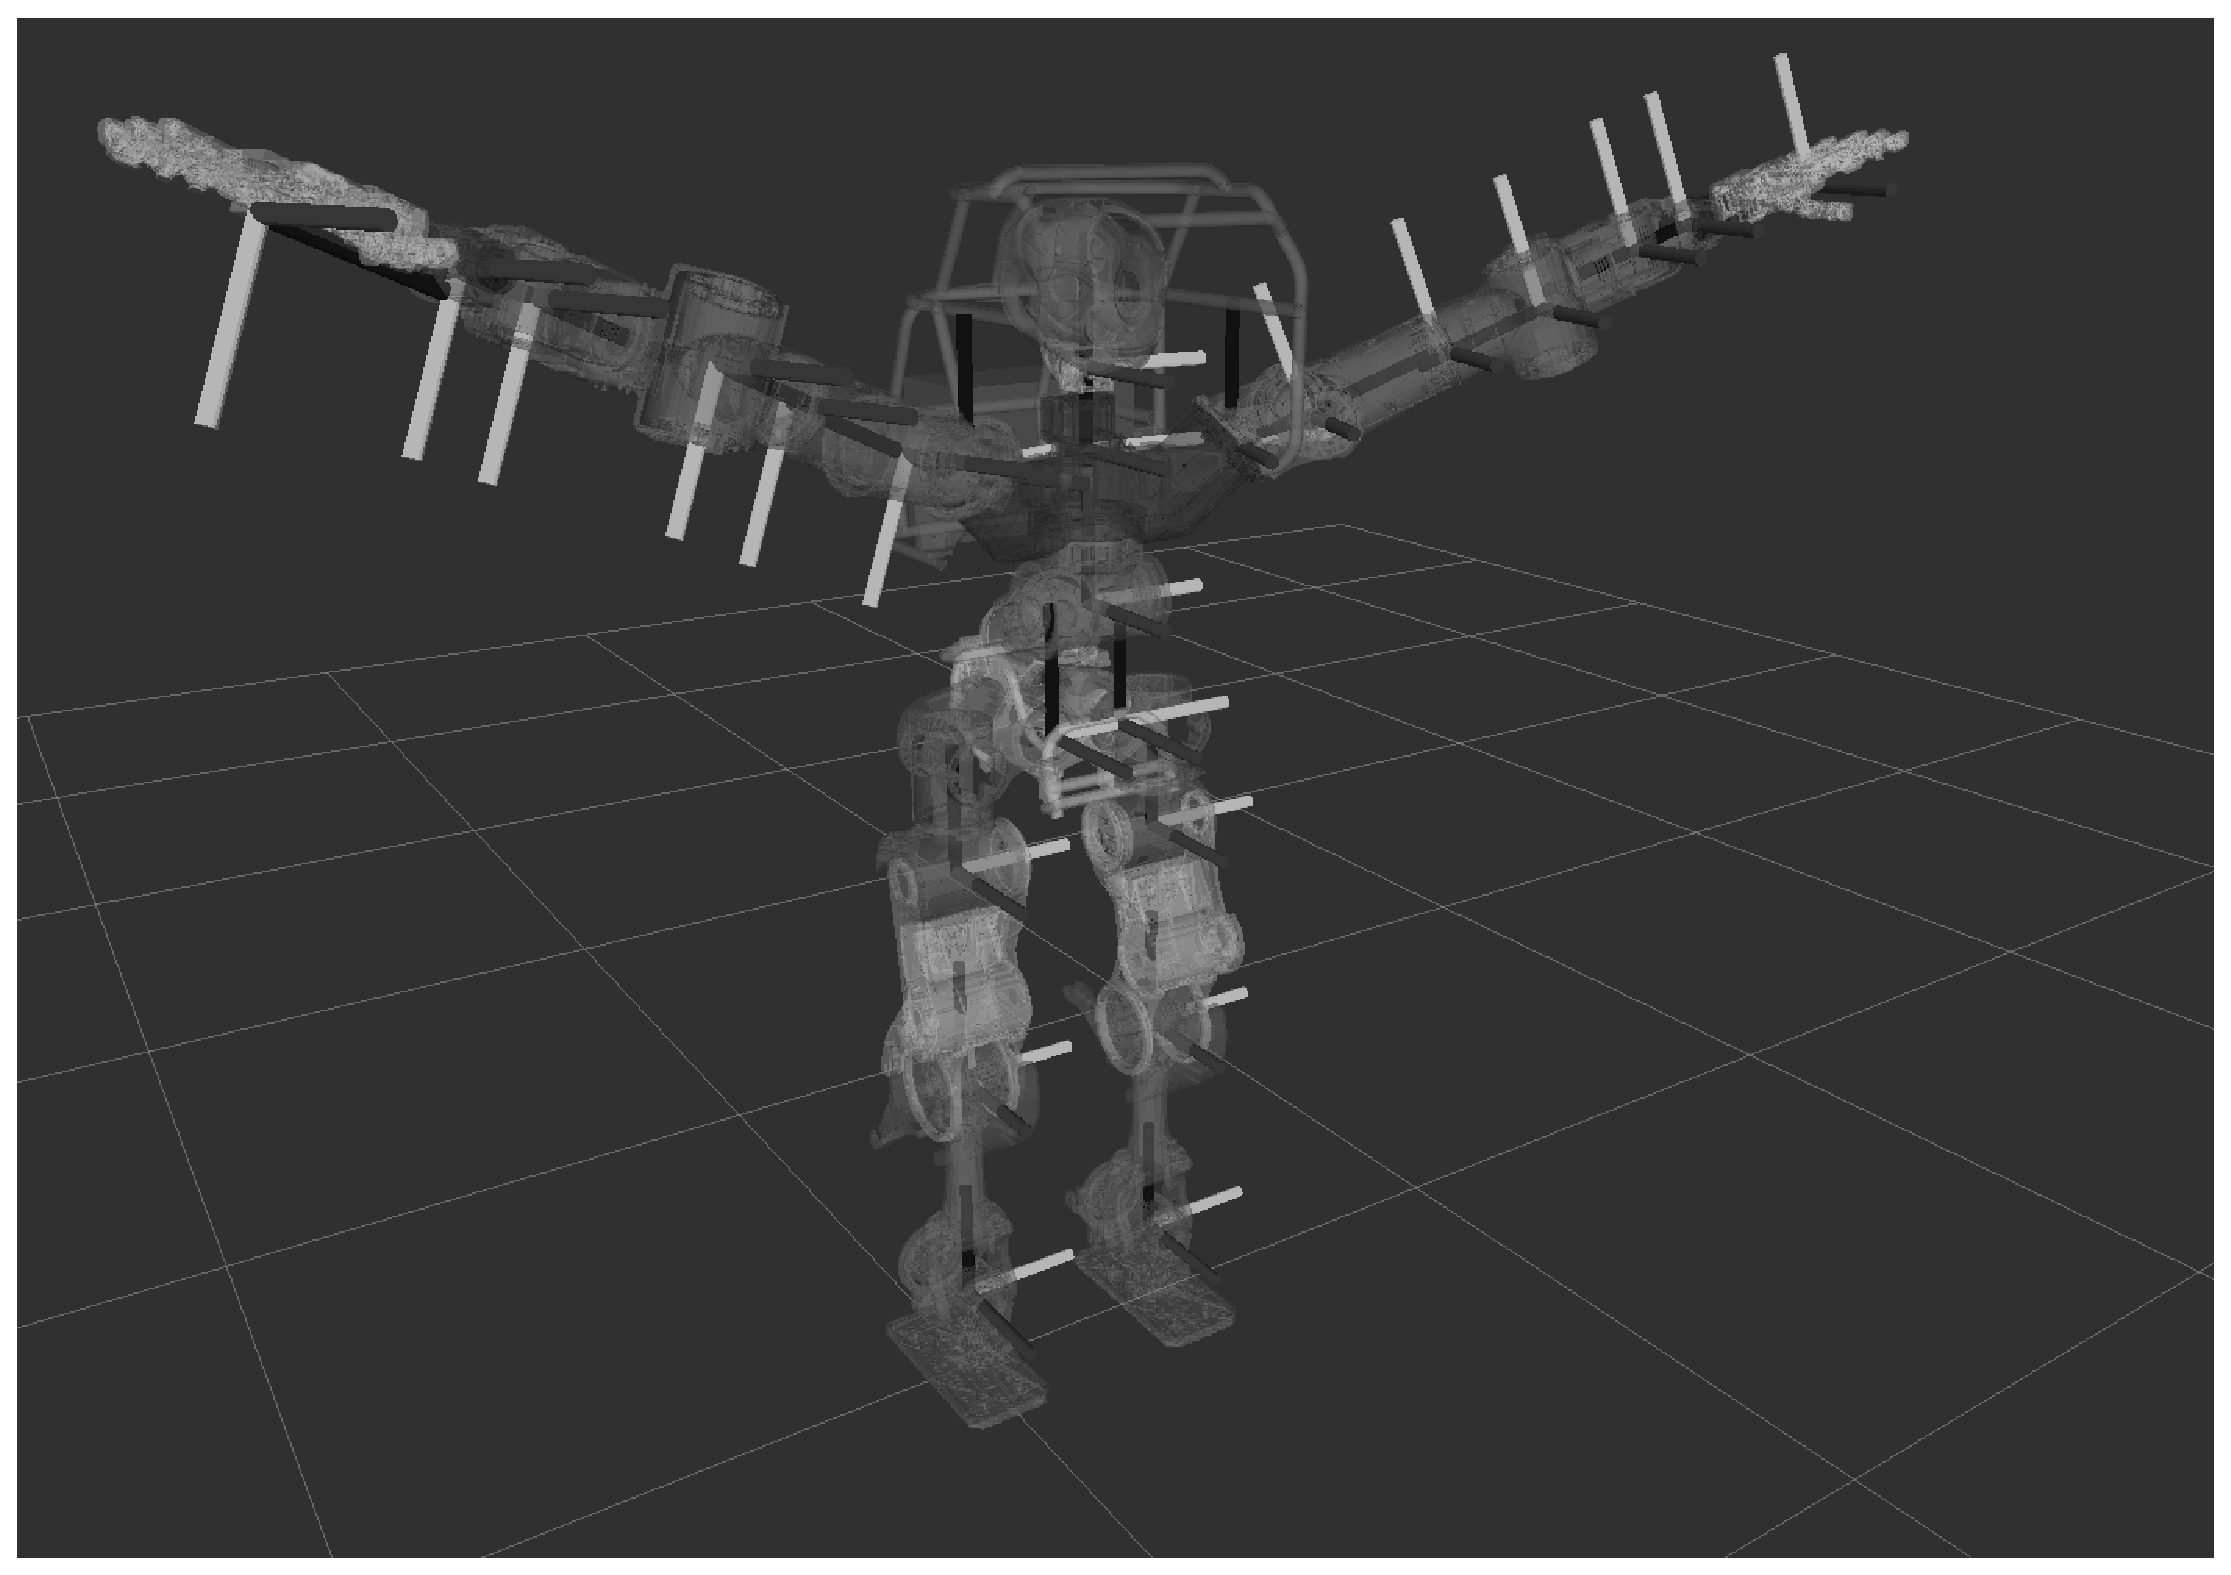
\includegraphics[width=\textwidth]{images/walkman_kinematics.eps} 
\caption{WALK-MAN robot kinematics and reference frames} 
\label{walkman_kinematics}
\end{figure}

\subsection{OpenSoT Tasks}
In \textbf{OpenSoT}, a task $T_i$ is in general defined as:
\begin{equation}
T_i = \T \left( \J_i,\, \de^*_i \right)
\end{equation}
For the solver, a task can be defined as a matrix and a vector, the task Jacobian and the task error respectively, which will get used by the solving algorithm. For the case of the QP stack,
\begin{equation}
T_i = \T \left( \A_i,\, \b_i \right)
\end{equation}
where $\A_i^T\A_i$ is the task Hessian and $\A_i^T\b_i$ the task gradient, in this case expressed by choosing the identity metric for the QP problem. In general, a different metric can be expressed by correctly designing the $W$ matrix the previous expression \todo{insert expression}, which will coincide to a different metric during the minimizatin of the $2$-norm of the residuals vector.

\subsubsection{Task operations: the Math of Tasks}
As previously specified, task operations can be used, together with the stacking operation, to build a complex stack out of simple stack definitions. These operations can be also defined using a simple semantic, which we call \emph{Math of Tasks} (Table \ref{table:mot}). 

\begin{table}[hbt]
   \begin{center}
   \begin{tabular}{| c | c | c | c |}
   \hline
   Operation & Symbol & Expression & Result \\\hline
   \cline{1-4}
   Stack                & $/$  & $S = T_1 / T_2$    & the stack $S$ gets created, $T_1$ has higher priority  \\\hline
   Augmentation         & $+$  & $T_3 = T_1 + T_2$  & the augmented task $T_3$ is created, $n_3 = n_1 + n_2$ \\\hline
   Applying Constraint  & $<<$ & $T_1 << C_0$       & the constraint $C_0$ is attached to the task $T_1$     \\\hline
   \end{tabular}
   \end{center}
   \caption{Math of Tasks: Operations and respective symbols}
   \label{table:mot}
\end{table}

\paragraph{Aggregated}
The aggregated task constructs an augmented Jacobian starting from a definition of more basic tasks. This allows to enforce soft priorities between tasks that get incorporated into the augmented task Jacobian. The formulation can be written as
\begin{eqnarray}
T_\text{agg} = & \T \left( \left[ \J_{1}^T\, \dotsc \,\J_n^T\right]^T, \quad \left[ \b_{1}^T\, \dotsc \,\b_{n}^T\right]^T \right)
\end{eqnarray}
where $\J_i \in \mathbb{R}^{n_i\times n_{\text{dofs}}}$
The aggregated task represents a way to impose soft priorities between different tasks. The relative priorities can be tuned by selecting a proper weight matrix, $\W_\text{agg} \in \mathbb{R}^{n_{\text{agg}}\times n_\text{agg}}$ with $n_\text{agg}=\sum_in_i$.
Considering a diagonal weight matrix $\W$
\begin{equation}
\W=\begin{bmatrix}
\beta_1                                             \\
&       \beta_2           &      & \text{{\huge{0}}}\\
&       &                 \ddots                    \\
&       \text{{\huge{0}}} &      & \beta_{n-1}      \\
&       &                 &      & \beta_n
\end{bmatrix}
\end{equation}
one would obtain the formulation from (\ref{eq:augmented_jacobian}).

\paragraph{SubTask}
The \emph{SubTask} allows to define tasks by selecting rows from a higher-dimensional task, $n_\text{sub}<n_\text{task}$. This allows to exert control only on the task dimensions of interest.

\begin{eqnarray}
T_\text{sub} = & \T \left( \left[ \J_{r_1}^T \dotsc \J_{r_p}^T \right]^T, \quad \left[ b_{r_1}^T \dotsc b_{r_p}^T \right]^T \right)
\end{eqnarray}
with
\begin{equation*}
r_i \in \left[1, n_\text{task} \right], r_i \neq r_j 
\end{equation*}
Where $r_i$ is a row index and $\J_{r_i}$ is a row vector from the original task, $b_{r_i}$ is the corresponding element from the vector $\b$.
This will result in a subtask of size $p \leq n$.

\paragraph{ActiveJointMask}
The \emph{Active Joint Mask} allows to effectively lock certain joints, meaning they will not get used by the specified task. It is implemented by substituting the columns of the joints to lock in the task Jacobian with a column of zeros, 

\begin{eqnarray}
T_\text{masked} = & \left( \left[ \J_{\text{masked},c_1} \dotsc \J_{\text{masked},c_n} \right], \quad \b \right)
\end{eqnarray}
where
\begin{equation*}
{\J_{\text{masked},c_i}=}
\begin{cases}
\J_{c_i} & \text{joint is active}\\
0_m & \text{joint is locked}
\end{cases}
\end{equation*}
 where $\J_{c_i}$ is the $i$-th column of the unmasked Jacobian, $0_m \in \mathbb{R}^{n_\text{task} \times 1}$.


\paragraph{Cartesian, CoM, MinimumCoMVelocity, MiminumCartesianVelocity}
\label{sec:cartesian_error}
It is possible to define a general Cartesian task as the \emph{aggregate} of a Cartesian position task and a Cartesian orientation task. The Cartesian task computes the (relative) Jacobian between any given base and distal links in the kinematic tree, $^b\J_d$. The Cartesian errors in position and orientation are computed respectively as: 
\begin{equation}
\begin{array}{l}
\e_p = \mathbf{p}_d - \mathbf{p}
\\
\\
\e_o = -(\eta_d \boldsymbol{\epsilon} - \eta \boldsymbol{\epsilon}_d + [\boldsymbol{\epsilon}_d\times] \boldsymbol{\epsilon})
\label{eq:cartesian_error}
\end{array}
\end{equation}
and the task is defined as:
\begin{equation}
\begin{array}{l}
T_{C,p} = \T \left(^b\J_{d,p}, \quad \mathbf{\dot{p}}_d + \mathbf{K}_p\e_p \right)
\\
\\
T_{C,o} = \T \left(^b\J_{d,o}, \quad \boldsymbol{\omega}_d +\mathbf{K}_o\e_o \right)
\label{cartesian_task}
 \end{array}
 \end{equation}
where $\mathbf{p}_d = [x_d \quad y_d \quad z_d]$ is the desired position and $\boldsymbol{\alpha}_d = [\eta_d \quad \epsilon_{1,d} \quad \epsilon_{2,d} \quad \epsilon_{3,d}]$ is the desired orientation expressed as a quaternion \cite{Nakanishi08operationalspace}, $\mathbf{K}_p$ and $\mathbf{K}_o$ are positive definite matrices and $\boldsymbol{\xi}_d = \left[ \boldsymbol{\dot{p}}_d \quad \boldsymbol{\omega}_d \right]$ is the desired Cartesian velocity for the end-effector.
A particular case is the \emph{CoM} task which is defined as a Cartesian position task. 
In both cases, the tasks can become minimum Cartesian velocity tasks by setting $\lambda=0$.

\paragraph{Interaction} \label{par:interaction} \todo{also in final version?}
The interaction task consists in force control through an admittance scheme. This task is built on top of the Cartesian task since pose and velocity references are generated from a wrench error:
\begin{equation}
\Delta\x = \mathbf{C} \left({^\text{b}\w_\text{d,ee}} - {^\text{b}\w_\text{m,ee}} \right )
\end{equation}
and 
\begin{equation}
{^\text{b}\w_\text{m,ee}} = \begin{bmatrix}
{^\text{b}\mathbf{R}_\text{ft}} & \mathbf{0}\\ 
\mathbf{0} & {^\text{b}\mathbf{R}_\text{ft}} 
\end{bmatrix}
\begin{bmatrix}
\mathbf{I} & \mathbf{0}\\ 
{^\text{ft}\mathbf{p}_\text{ee}\times} & \mathbf{I} 
\end{bmatrix}{^\text{ft}\w_\text{m,ft}}
\end{equation}
where ${^\text{b}\w_\text{d,ee}}$ is the desired wrench that the robot has to exert to the environment, ${^\text{ft}\w_\text{m,ft}}$ is the wrench that the robot is exerting to the environment measured on the force/torque sensor, ${^\text{b}\mathbf{R}_\text{ft}}$ is the rotation from the base link to the force/torque reference frame, ${^\text{ee}\mathbf{p}_\text{ft}\times}$ is the skew symmetric matrix computed from the distance between the force/torque reference frame and the end-effector reference frame, $\mathbf{C}$ is a positive definite compliance matrix. The computed $\Delta\x$ is used as feed-forward term and integrated as reference term for the Cartesian task.

\paragraph{MinimumEffort}
The minimum effort task is defined in joint space as:
\begin{equation}
T_\text{mineffort} = \T \left(\I, \quad \alpha_g\nabla(g(\q)^Tg(\q))\right)
\end{equation}
where $g(\q)$ are the torques due to gravity computed through Iverse Dynamics. The gradient is computed numerically by means of two-point estimation and the Hessian is set to be the identity, so as to effectively implement a \emph{Gradient Projection Method} \cite{Rosen1960-gm}. 

\paragraph{Manipulability}
The manipulability task is again defined in joint space as:
\begin{equation}
T_\text{manip} = \T \left(\I, \quad -\alpha_g\nabla(h(\q))\right)
\end{equation}
with
\begin{equation}
h(\q) = det\left(\sqrt{\J(\q)^T\J(\q)}\right)
\end{equation}
being the manipulability index of the robot. As for the minimum effort task, the gradient is computed numerically. The minus sign  is worth noticing since the task is a maximization of the chosen manipulability index of the robot.

\paragraph{MinimizeAcceleration} \todo{also in final version?}
The minimize acceleration task is also defined in joint space as:
\begin{equation}
T_\text{minacc} = \left(\I, \quad \lambda\dq_\text{prev}\right)
\end{equation}
This task will try to minimize the change in velocity in joint space. When the $\lambda$ of the task is equal to $\frac{1}{dT}$, it will become independent from the time step size and will effectively be a first order approximation of joint acceleration minimization.

\paragraph{Postural}
A postural task is defined in joint space as:
\begin{equation}
T_p = \left(\I, \quad  \dq_d + \lambda(\q_d - \q)\right)
\label{sec:postural_task}
\end{equation}
The task can become a minimum velocity task by setting $\lambda=0$ and $\dq_\text{d} = 0$, as in this case the cost function is reduced to $\left \| \dq \right \|_\textbf{W}$.

\todo{insert class diagram?}
%\begin{figure}
%  \centering
%  \vspace*{0.05in}
%    \includegraphics[width=0.47\textwidth]{images/open_sot_inherit}
%    \caption{Class diagram and inheritance in \emph{OpenSoT}}\label{open_sot_inherit}
%    \vspace*{-0.2in}
%\end{figure}

\subsubsection{Constraints and Bounds}
Constraints model equalities and bilateral/unilateral inequalities. 
A generic unilateral constraint of the form
\begin{equation}
\A_{c,1}\dq \leq \b_{c,1} 
\end{equation}
can be expressed using the simple syntax: 
\begin{equation}
\C\left( \A_c,\, \b_c \right)
\end{equation}
Bilateral constraints and unilateral and bilateral bounds can be expressed in terms of unilateral constraints according to Table \ref{table:constraints_and_bounds}.

\begin{table}[hbt]
   \begin{center}
   \begin{tabular}{| c | c | c | c |}
   \hline
   Constraint & Equation & Syntax & Equivalent Syntax \\\hline
   \cline{1-4}
   bilateral constraint & $\b_{l} \leq \A_{c}\dq \leq \b_{u}$ & $\C_\text{bilateral}\left( \A_c, \, \b_{c,l}, \, \b_{c,u} \right)$ & $\C \left( \left[ \A_{c}^T \, -\A_{c}^T \right]^T, \, \left[ \b_{c,u}^T \, \b_{c,l}^T \right]^T \right)$ \\\hline
   unilateral bounds     & $\dq \leq \b_{c,u}$       & $\B\left( \b_{c,u} \right)$ & $\C\left(\I_{n_\text{dofs}}, \, \b_{c,u}^T \right)$ \\\hline
   bilateral bounds     & $\b_{l} \leq \dq \leq \b_{u}$       & $\B_\text{bilateral}\left( \b_{c,l}, \, \b_{c,u} \right)$ & $\C\left(\left[ \I_{n_\text{dofs}}  \, -\I_{n_\text{dofs}} \right]^T, \, \left[ \b_{c,u}^T \, \b_{c,l}^T \right]^T \right)$ \\\hline
   \end{tabular}
   \end{center}
   \caption{Constraints and bounds. Transforming unilateral constraints and bounds from upper bounds to lower bounds is trivial and therefore not included in the table}
   \label{table:constraints_and_bounds}
\end{table}

Constraints and bounds can be applied to a single task (i.e. $T_i << \C$) or to the whole stack (i.e. $S << \C$): applying constraints to the stack is equivalent to applying them to every task in the stack.
We will call the former \emph{local} constraints, while we will refer to the latter as \emph{global}. In general, when a \emph{local} constraint is applied to a certain task, it should be applied also to all its lower priority tasks in the stack to make sure that it will be enforced in the final solution. There are, anyway, conditions when a constraint does not need to be enforced directly to lower priority tasks, since its enforcement is implicit in keeping optimality of the higher priority tasks.
Consider a task $T_i=\T\left(J_i,\de^*_i\right)$, $\J \in \mathbb{R}^{m\times n}$ with $rank(\J) = m$, a stack $S$ composed of $n$ tasks, and a constraint $C_j=\C\left(\A_{c,j},\,\b_{c,j}\right)$. If we apply the constraint to the task $T_i << C_j$, if \todo{it can be written more coincisely}
\begin{equation}
rank\left ( \begin{bmatrix}
\J_i\\ 
\A_j
\end{bmatrix} \right ) = m
\end{equation}
then $C_j$ can be applied as a local constraint to $T_i$, and it will automatically be enforced on lower priority tasks up to the final solution $\dq_n^*=\dq_d$ ($T_j \forall j>i$) since it will be implicit in the solution $\dq_i$.

\paragraph{Aggregated}
The aggregated constraint performs merging of a list of constraints into a single constraint, in particular piling the equalities and inequalities constraints, and merging the bounds as follows:
\begin{eqnarray}
C_{\text{agg}} = & \C\left( \left[ \A_{c,1}^T \quad \A_{c,2}^T \right]^T,\quad \left[ \b_{c,1}^T \quad \b_{c,2}^T \right]^T \right) \\
b_{\text{agg}} = & \left( \max\left(\textbf{l}_1,\textbf{l}_2 \right), \quad \min\left(\textbf{u}_1,\textbf{u}_2\right) \right)
\end{eqnarray}

\paragraph{ConvexHull}
The CoM is bounded to lay inside the convex hull defined by the contacts with the environment (Figure \ref{com_ch}), where we can write 
\begin{equation}
C_\text{CH} = \C \left( 
\begin{bmatrix}     a_0     & b_0     \\ 
                    \vdots  & \vdots  \\
                    a_{n-1} & b_{n-1} \\
\end{bmatrix}, \quad 
\begin{bmatrix} -c_0     \\ 
                \vdots   \\
                -c_{n-1} \\
\end{bmatrix} \right) = \C \left( \A_\text{CH},\, \b_\text{CH} \right)
\end{equation}
with $a_i$,$b_i$,$c_i$ coefficients of the implicit equation of the line $a_ix+b_iy+c_i=0$, bounding the convex hull. These lines are  expressed in a frame attached to the CoM and parallel to the inertial frame, and are obtained by finding the coefficients of a line passing through two consecutive points of the convex hull of the support polygon. The convex hull is obtained by creating a hull of a point cloud of contact points between the foot and the ground, which can be obtained by skin sensors or, in current implementation, by the foot model assuming full-foot contact with the ground.
\begin{figure}[hb!]
  \center
  \vspace*{0.05in}
    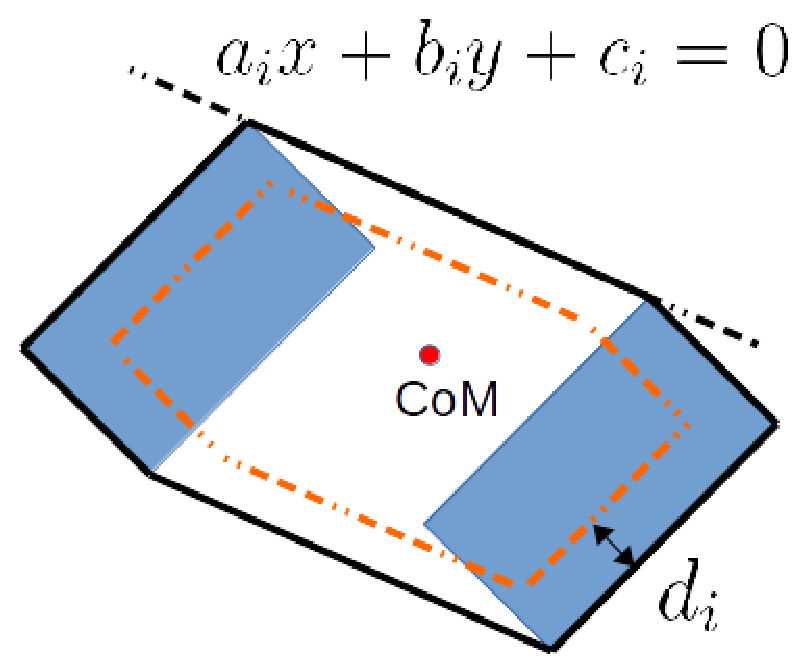
\includegraphics[width=0.3\textwidth]{images/wholebody/com_ch}
    \caption{The convex hull constraint for the CoM}\label{com_ch}
    %\vspace*{-0.2in}
\end{figure}
In order to keep the vector $\b_\text{CH}$ expressed in the same units in which the points in the Convex Hull are expressed with respect to a certain frame, then the convex hull lines coefficients are normalized, so that for the $i$'th line, the coefficients will be scaled by the factor $d_i=\sqrt{a_i^2+b_i^2}$.



\paragraph{BilateralConstraint}
This constraint is a generic constraint that can be built on the fly manually specifying a constraint matrix, $\A_\text{user}$, and upper and lower bounds $\b_{l,\text{user}}$, $\b_{u,\text{user}}$
\begin{eqnarray}
C_{\text{bc}} = & \C_\text{bilateral} \left( \A_\text{user},\, \b_{l,\text{user}} ,\, \b_{u,\text{user}} \right)
\end{eqnarray}

\paragraph{CartesianPositionConstraint}
The constraint implements limits on the Cartesian position of any feature on the robot body with respect to a defined hull in Cartesian space.

\paragraph{CoMVelocity}
This constraint implements limits on the Cartesian velocity of the \emph{CoM} w.r.t. another link, or the inertial frame
\begin{eqnarray}
C_\text{C,p} = & \left( ^{l}\J_{CoM}, \quad ^{l}\dx_{\text{max,CoM}} \right)
\end{eqnarray}

%To limit the Cartesian velocity of any link w.r.t. another link, or the inertial frame, the generic \emph{BilateralConstraint} can be used, with $A=\J,b_{ub}=\x_\text{max},b_{lb}=\x_\text{min}$.

\paragraph{TaskToConstraint}
This constraint allows to transform any task into a constraint. It is applicable for the cases when a certain task can be performed with zero error, e.g. the loop closure equation between the two feet of a humanoid robot in a double support stance.

\paragraph{JointLimits}
The joints limit constraint is one of the fundamental constraints to use in the real robot. It prevents to hit the joint limits reaching them at zero speed: 
\begin{equation}
b_\text{JointLimits} = (\sigma\left( \q_\text{min} - \q \right),\quad \sigma\left( \q_\text{max} - \q \right))
\end{equation}
with $\left(\q_\text{min}, \ \q_\text{max} \right)$ the joint limits.


\paragraph{JointVelocity}
Joint velocity limits permits to generate trajectories with bounded velocities:
\begin{equation}
b_\text{JointVelocity} = \left( -\sigma \dq_\text{max}\Delta t,\quad \sigma \dq_\text{max}\Delta t \right)
\end{equation}
with $\dq_\text{max}$ the maximum allowed joint velocity.
%with $\text{u}_\text{j\_lims}$ and $\text{l}_\text{j\_lims}$ the $\dq$
%where $\alpha_i \leq \alpha_{i+1}$ scales the bounds in order to implement a simple velocity allocation scheme between tasks at different priority levels.

\paragraph{Dynamic Filter} \todo{cut from here? Ask Enrico}
One of the fundamental problems in IK is that some assigned Cartesian reference trajectories might be dynamically unfeasible by the robot. This means that the robot might get damaged since the required joint torque for a certain motion could be too high. Various techniques have been presented in the past to avoid this problem, one of the most famous is the \emph{Dynamic Filter} \cite{Yamane:04}. This technique basically uses an ID step to filter the generated joint accelerations from the IK solution. 

The \emph{Dynamic Filter} can be formulated as a constraint. The dynamics of the robot can be written as:
\begin{equation}
\mathbf{M}(\mathbf{q})\mathbf{\ddot{q}} + \mathbf{C}(\mathbf{q},\mathbf{\dot{q}})\mathbf{\dot{q}} + \mathbf{G}(\mathbf{q}) = \boldsymbol{\tau} - \mathbf{J}^T_c\mathbf{f}_c
\end{equation}
where $\mathbf{M}(\mathbf{q})$ is the joint space inertia matrix, $\mathbf{C}(\mathbf{q},\mathbf{\dot{q}})$ takes into account centrifugal and Coriolis terms, $\mathbf{G}(\mathbf{q})$ are the gravity torques, $\boldsymbol{\tau}$ are the joint torques and $\mathbf{J}^T_c\mathbf{f}_c$ are the torques due to contacts (that we measure on the force/torque sensors). 
Considering an acceleration level control and taking into account that each joint can provide $\left[\tau_{\text{i,min}}, \ \tau_{\text{i,max}} \right]$, it is possible to write the constraint as:
\begin{equation}
\mathbf{D}(\mathbf{q, \dot{q}}) + \boldsymbol{\tau}_\text{min}\leq \mathbf{M}(\mathbf{q})\mathbf{\ddot{q}} \leq  \mathbf{D}(\mathbf{q, \dot{q}}) + \boldsymbol{\tau}_\text{max}
\end{equation}
with $\mathbf{D}(\mathbf{q, \dot{q}},\mathbf{f}_c) = -\left(\mathbf{C}(\mathbf{q},\mathbf{\dot{q}})\mathbf{\dot{q}} + \mathbf{G}(\mathbf{q}) - \mathbf{J}^T_c\mathbf{f}_c \right )$. In this work we are considering velocity level control, so it is possible to approximate the joint acceleration $\mathbf{\ddot{q}}$ as:
\begin{equation}
\mathbf{\ddot{q}} = \frac{\mathbf{\dot{q}}-\mathbf{\dot{q}}_\text{prev}}{\Delta T}
\end{equation}
then the constraint can be rewritten at the velocity level as:
\begin{equation}
\Delta T \left(\mathbf{D}(\mathbf{q}, \mathbf{\dot{q}}) + \boldsymbol{\tau}_\text{min}\right ) + \mathbf{M}(\mathbf{q})\mathbf{\dot{q}}_\text{prev} \leq
\mathbf{M}(\mathbf{q})\mathbf{\dot{q}} 
\leq  \Delta T \left(\mathbf{D}(\mathbf{q}, \mathbf{\dot{q}}) + \boldsymbol{\tau}_\text{max}\right)+ \mathbf{M}(\mathbf{q})\mathbf{\dot{q}}_\text{prev}
\label{robot_dynamics_constraint}
\end{equation}
A similar idea was presented also in \cite{park1998-ib} but contact forces were not taken in consideration.
Practically speaking, as we did for other constraints, it is useful to have a scaling factor $\sigma \ \in \ \left(0, \ 1 \right]$ in front of the constraint:
\begin{equation}
\sigma \left(\Delta T \left(\mathbf{D}(\mathbf{q}, \mathbf{\dot{q}}) + \boldsymbol{\tau}_\text{min}\right ) + \mathbf{M}(\mathbf{q})\mathbf{\dot{q}}_\text{prev} \right)\leq
\mathbf{M}(\mathbf{q})\mathbf{\dot{q}} 
\leq  \sigma \left(\Delta T \left(\mathbf{D}(\mathbf{q}, \mathbf{\dot{q}}) + \boldsymbol{\tau}_\text{max}\right)+ \mathbf{M}(\mathbf{q})\mathbf{\dot{q}}_\text{prev}\right)
\label{robot_dynamics_constraint_2}
\end{equation}

%\subsection{OpenSoT Solver}
%\emph{OpenSoT} provides a class to implement different \emph{Solvers} that uses the classes \emph{Tasks}, \emph{Constraints} and \emph{Bounds} to solve the IK problem for a desired control type. The actual solver  supported in \emph{OpenSoT} is based on (\ref{eq:sot_full}) and is currently supporting  only velocity based task and Constraints.  Therefore \emph{velocity control} is the available control type in the current state of implementation while other type of solvers which support different control modalities are due to be integrated soon.
%The solver uses qpOASES \cite{ferreau2013}, an open-source C++ implementation of an on-line active set strategy \cite{ferreau2008online}, part of the ACADO suite. qpOASES implements an automatic regularization technique (therefore there is no need for explicit singularity avoidance and escaping) and warm-start functionalities. The solver permits to define any type of stack and it handles the bounds in a global way. To test the performances of the solver we have prepared a benchmark were a variable sized stack is created and solved. The lowest priority task is always a postural task (\ref{sec:postural_task}) while the others are Cartesian tasks (\ref{sec:cartesian_task}), bounds on joint limits and velocities are also added to the optimization. 
%\begin{table}
%\centering
%\vspace{1mm}
%\caption{Solver Time}
%\vspace*{0.1in}
%\begin{tabular}{|c|c|c|}
% \hline
% \# Stacks & Tasks & Time [s] \\
% \hline
% 2 & postural, CoM& 0.003 \\
% \hline
% 3 & postural, CoM, left\_arm & 0.005 \\
% \hline
% 4 & postural, CoM, left\_arm, right\_arm & 0.007 \\
% \hline
%\end{tabular}
%\caption*{Time to solve different stacks of tasks. Note that left\_arm and right\_arm share part of the kinematic chain in the torso}
%\label{table:time}
%\vspace*{-0.2in}
%\end{table}
%Table \ref{table:time} shows the results to solve one control step of optimization\footnote{These results were obtained using a Intel Core i7 with 6GB of RAM} for 29 variables.% In Listing \ref{lst:workflow} a typical workflow using \emph{OpenSoT} types is shown.

%\begin{lstlisting}[language=C++, caption=SoT Workflow, basicstyle=\footnotesize, label={lst:workflow}]
%/* creating Tasks, Constraints and global Bounds */
%Vector<TaskPtr> stack;
%TaskPtr comTask = new CoM();
%comTask.constraints.push_back(new CoMVelocity());
%stack.push_back(comTask);
%stack.push_back(new Cartesian(l_wrist,l_sole));
%ConstraintPtr jLim = new JointLimits();
%ConstraintPtr jVel = new JointVelocities(0.3);
%ConstraintPtr bounds = new Aggregated(jLim, jVel);
%/* creating the solver */
%SolverPtr solver = new solverQP(stack, bounds);
%/* control Loop */
%while(true) {
%    q = senseAndUpdateModel();
%    for(i = 0; i < stack.size(); ++i) 
%        stack[i]->update(q);
%    bounds->update(q); 
%    solver->solve(dq);
%    q += dq;
%    move(q);}
%\end{lstlisting}
%\vspace*{-0.2in}

\subsubsection{Self-Collision Avoidance Constraint}
\label{sec:collision_avoidance}
In our framework, the self-collision avoidance constraint will be formulated as an inequality constraint for each task in the IK Problem to guarantee the safety of the robot. The basic idea is to calculate the minimum distance between every link pair in every control loop and obtain a list of several closest link pairs according to these minimum distances. For each of these link pairs of interest, we try to control the relative velocity of the one link with respect to the other in the direction connecting the closest points on the two links respectively, which is called velocity damping firstly introduced in \cite{1087982} and reformulated inside the SoT \cite{kanehiro2008local}, to avoid the potential collision between them. 

So, to accelerate the computation of minimum distance of each link pair, we should employ some simpler collision model for each link first. In our paper, the capsule, sphere-swept line, is chosen among a lot of types of bounding volumes because of the convenience of the computation. As shown in Figure \ref{fig:link_pair}, the minimum distance of the link pair can be just considered as the minimum distance between the inner line segments minus the sum of the radii of the capsules for the two links respectively. The method proposed in \cite{el_khoury2013-rp} is employed to generate the minimum bounding capsule for each of exact link body geometries represented by mesh. Furthermore, the minimum distance between a capsule pair and the shortest points on them can be easily obtained by using the Flexible Collision Library (FCL) \cite{6225337}. FCL is a fully templated library which aims at general proximity calculation and collision detection on various types of collision geometries such as axis-aligned bounding box (AABB) and oriented bounding box (OBB). As of version $3.0$ of the library, the capsule collision geometry has been added \cite{knese2014msc}.  

\begin{figure}[!ht]
    \centering
    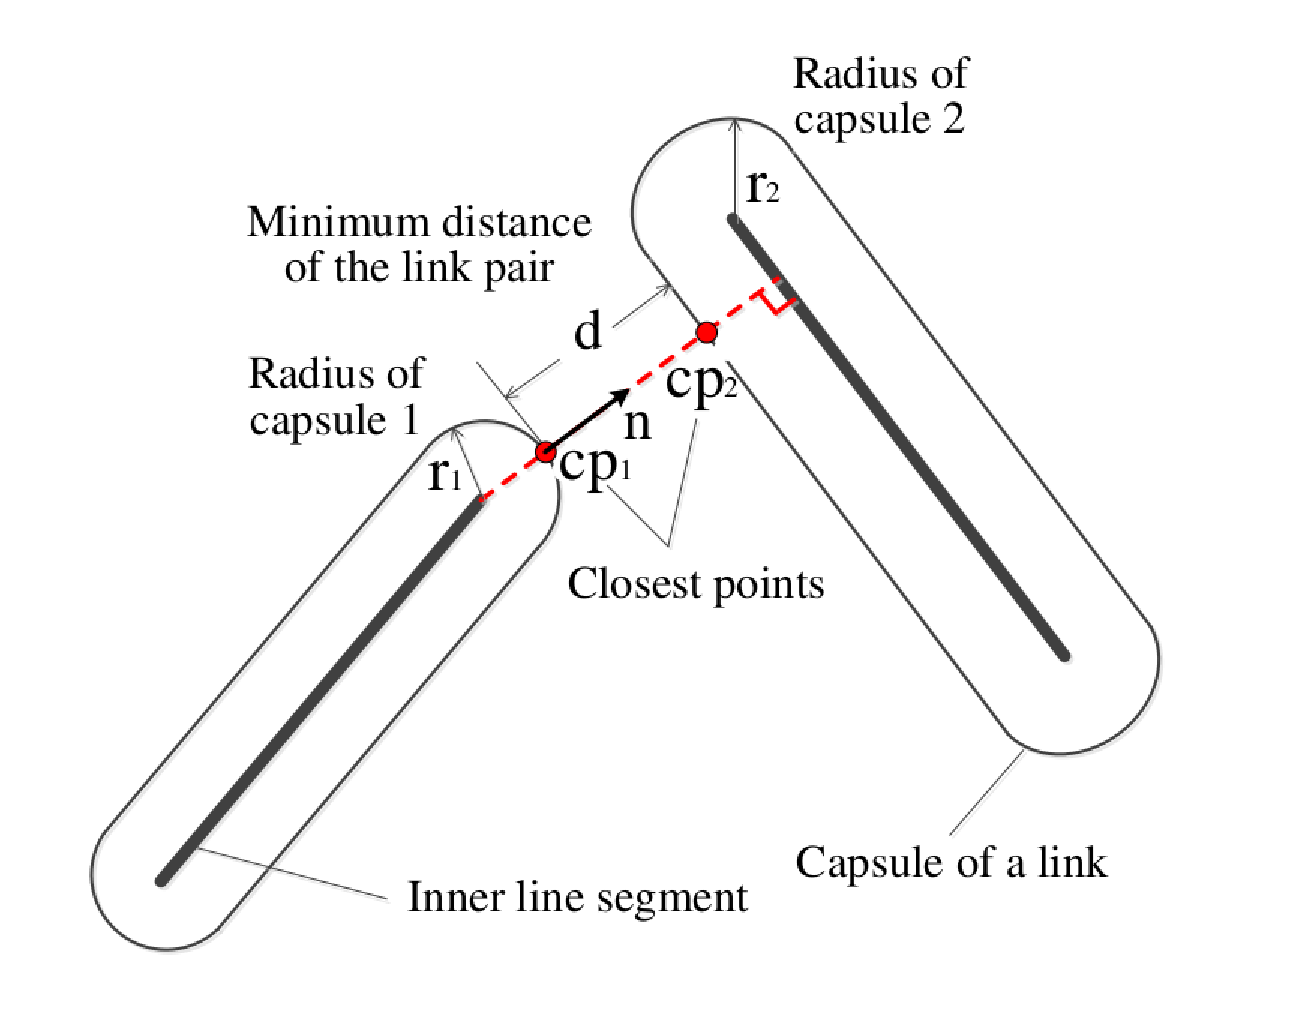
\includegraphics[width=0.5\textwidth]{images/wholebody/link_pair}
    \caption{Schematic diagram of the collision avoidance constraint on a capsule pair representing the collision model for a link pair}\label{fig:link_pair}
    \vspace{-3mm}
\end{figure}

Once the closest points are computed, for instance, $ \bm{cp}_1 $ and $ \bm{cp}_2 $ shown in Figure \ref{fig:link_pair}, the relative motion of the capsule pair is going to be restricted in the direction:

\begin{equation} 
\label{eq:unit_vector}
\begin{array}{c}
\bm{n} = \dfrac{\bm{cp}_2-\bm{cp}_1}{\Arrowvert \bm{cp}_2-\bm{cp}_1 \Arrowvert} 
\end{array}
\end{equation}

Where the distance $ \Arrowvert \bm{cp}_2-\bm{cp}_1 \Arrowvert $ is calculated according to the Euclidean L2-norm. So, the relative velocity constraint in this direction can be formulated as follows:

\begin{equation} 
\label{eq:SCA_constraint}
\begin{array}{c}
\bm{n}^{T}[\bm{J}(\bm{cp}_1,\bm{q})-\bm{J}(\bm{cp}_2,\bm{q})]\dot{\bm{q}} \leq \varepsilon \dfrac{d-d_s}{\Delta t} 
\end{array}
\end{equation}
 
 In (\ref{eq:SCA_constraint}), $ \bm{J}(\bm{cp}_1,\bm{q}) $ and $ \bm{J}(\bm{cp}_2,\bm{q}) $ refer to the Jacobian matrices of the frames located at the closest points $ \bm{cp}_1 $ and $ \bm{cp}_2 $ respectively with respect to the base frame. Since the relative location of the capsule relative to the corresponding link frame is fixed, these two Jacobians can be obtained based on the Jacobians of their link frames by some simple transformation. It is worth noting that only the linear velocity component of the Jacobian (the first three rows) is taken into account in this case. Then, the formula $ [\bm{J}(\bm{cp}_1,\bm{q})-\bm{J}(\bm{cp}_2,\bm{q})]\dot{\bm{q}} $ can be considered as the relative velocity of the capsule pair. In addition, $ d_s $ is the safety distance which is the shortest distance allowed for the capsule pair, $ \Delta t $ denotes the control loop period, and $ \varepsilon $ indicates the gain value which is used to smoothly reduce the relative approaching velocity at which the threshold distance is reached. So, the inequality in (\ref{eq:SCA_constraint}) means the velocity projected from the original relative velocity of the capsule pair onto the direction connecting the closest points on the capsules would never make the distance between them smaller than the safety distance $ d_s $, which is then used to avoid potential collision between the corresponding link pair. Furthermore, for multiple link pairs, the constraint formulation evolves to:


\vspace{-2mm}
    \begin{equation} 
        \label{eq:SCA_constraint_matrix}
        \begin{array}{rcl}
            \left( \begin{array}{c}
                {\bm{n}_1}^{T}\bar{\bm{J}_1}  \\
                \rotatebox{90}{$\cdots$}  \\
                {\bm{n}_k}^{T}\bar{\bm{J}_k}  \end{array} \right) \dot{\bm{q}} &  \leq  &
            \left( \begin{array}{c}
            \bar{d}_1  \\
\rotatebox{90}{$\cdots$}  \\
\bar{d}_k  \end{array} \right) \\

\bm{N} \ \dot{\bm{q}} &  \leq  & \bm{D} \\

\text{where} \ \ \ \ \ \ \ \ \ \bar{\bm{J}_i} & = & \bm{J}(\bm{cp}_{1,i},\bm{q})-\bm{J}(\bm{cp}_{2,i},\bm{q}) \\

\text{and} \ \ \ \ \ \ \ \ \ \ \ \ \bar{d_i} & = & \varepsilon_i \dfrac{d_i - d_{s,i}}{\Delta t}
\end{array}
\end{equation}

In this case, in order to add the self-collision avoidance constraint for $ k $ pairs of links in the IK Problem, the inequality constraint of every task should be replaced by $ \bm{N} \dot{\bm{q}} \leq \bm{D} $ in (\ref{eq:SCA_constraint_matrix}).


\subsection{Robust IK Solver}
\label{sec:robust_ik_solver}
\textbf{OpenSoT} provides a class to implement different \emph{Solvers} that use the classes \emph{Tasks}, \emph{Constraints} and \emph{Bounds} to solve the IK problem for a desired control type.
As mentioned before, the IK is a fundamental part in the control scheme as it maps the desired references in the operational space to desired references in joint space. This is a potentially dangerous step for many reasons that depend largely on the algorithm chosen to solve the IK problem.
For this reasons an IK solver must be \emph{robust} and we define two main characteristics: \emph{singularity robustness} and \emph{constraints/bounds handling}.
The first one is required anytime the robot is near the kinematics singularities and the algorithm has to assure that no high joint velocities are generated.
The latter is fundamental to prevent that a task potentially damages the robot. 

Considering these requirements, we developed the standard IK solver provided with \textbf{OpenSoT} based on a sequence of QP optimizations with the possibility to specify \emph{hard} and \emph{soft} priorities between tasks as well as linear constraints and bounds. 
The solver is based on the framework (\ref{eq:sot_full}):\todo{review for clearer explanation of damping}
\begin{equation} 
\label{optimization_problem2}
\begin{array}{c}
\underset{\dot{\mathbf{q}}}{\operatorname{argmin}} \ \Arrowvert \mathbf{J}_i \dot{\mathbf{q}}_i-\mathbf{v}_{d,i} \Arrowvert_{\mathbf{W}} + \lambda \Arrowvert \dot{\mathbf{q}}_i \Arrowvert\\
s.t. \ \mathbf{c}_\text{l,i} \leq \mathbf{A}_i\dot{\mathbf{q}}_i \leq \mathbf{b}_\text{u,i}\\
\ \ \ \mathbf{b}_\text{l} \leq \mathbf{A}\dot{\mathbf{q}}_i \leq \mathbf{b}_\text{u}\\
\ \ \ \mathbf{u}_\text{l} \leq \dot{\mathbf{q}}_i \leq \mathbf{u}_\text{u}\\
\ \ \ \mathbf{J}_{i-1}\dot{\mathbf{q}}_{i-1} = \mathbf{J}_{i-1}\dot{\mathbf{q}}_i\\
\ \ \ \vdots \\
\ \ \ \mathbf{J}_{0}\dot{\mathbf{q}}_{0} = \mathbf{J}_{0}\dot{\mathbf{q}}_i
\end{array}
\end{equation}
where $\mathbf{J}_i$ and $\mathbf{v}_{d,i}$ are respectively the Jacobian and the desired velocity reference for i-th task, $\lambda$ is a weight for the damping correction, $\mathbf{A}_i$, $\mathbf{c}_\text{l,i}$ and $\mathbf{c}_\text{u,i}$ are constraints present only in the i-th task, $\mathbf{A}$, $\mathbf{b}_\text{l}$ and $\mathbf{b}_\text{u}$ are global constrains as well as $\mathbf{u}_\text{l}$ and $\mathbf{u}_\text{u}$ are bounds that are present in all the tasks. 
The final set of constraints represent the optimality conditions that comes from the higher priority level tasks in the stack. In our IK solver all the optimality conditions are set automatically given the IK Problem while the other constraints are set by the user.
As shown in \cite{nakamura1990-tp} the second term in the cost function guarantees the robustness near kinematics singularities, the $\lambda$ gain can be chosen according to different criteria). Bounds and constraints are mandatory in order to be robust to joint limits and joint velocity/acceleration/torque limits.
Conceptually, the IK solver is divided in two main parts: the \emph{front-end} and the \emph{back-end}.
The \emph{front-end} takes an IK Problem and prepare all the QP Problems that needs to be solved considering priorities, local and global constraints and bounds. The \emph{back-end} consists of the underneath QP Solver that solves the single QP Problem. Tasks, constraints and bounds are defined as \emph{pointers} and updated outside the solver at every step.

\subsubsection{Back-End}
As mentioned before, the \emph{back-end} is based on a popular QP solver library called \emph{qpOASES} \cite{ferreau2013} which implements an active-set approach to handle inequality constraints. The library provides also a \emph{warm-start} and a \emph{hot-start} approach to solve the QP Problem. Basically, in the \emph{warm-start}, an initial guess from the previous solution and previous active set is used. This permits to speed up the computation with respect to a classical solution (that we call \emph{initialization} because it has to be performed at least in the beginning).
In the \emph{hot-start} also the previous decomposition of the matrix for the KKT conditions is used to speed up computation. 

% REMOVED 05/02/16
% \begin{figure}[htb] 
% \vspace{2 mm}
% \centering 
% 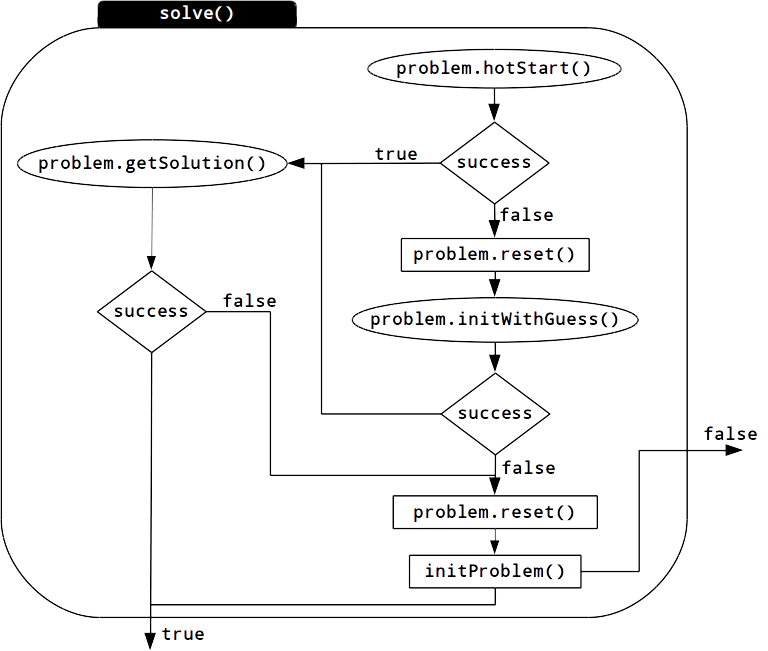
\includegraphics[width=0.5\textwidth]{images/wholebody/QPOasesProblem_solve2.png} 
% \caption{In the \emph{back-end}, if the \emph{hot-start} fails, then \emph{warm-start} is attempted. If also \emph{warm-start} fails than a new \emph{initialization} of the problem is performed} 
% \label{qpOasesProblemSolve}
% \end{figure}

When a QP has to be solved, the \emph{back-end} first tries to solve the problem using the \emph{hot-start}, if an error occurs then the \emph{warm-start} is used. If also the \emph{warm-start} fails a new \emph{initialization} of the QP Problem is performed. If also the \emph{initialization} fails then the solver will not generate a solution and notify the user by returning a \emph{false} value.

% REMOVED 05/02/16
% \begin{figure}[htb] 
% \centering 
% 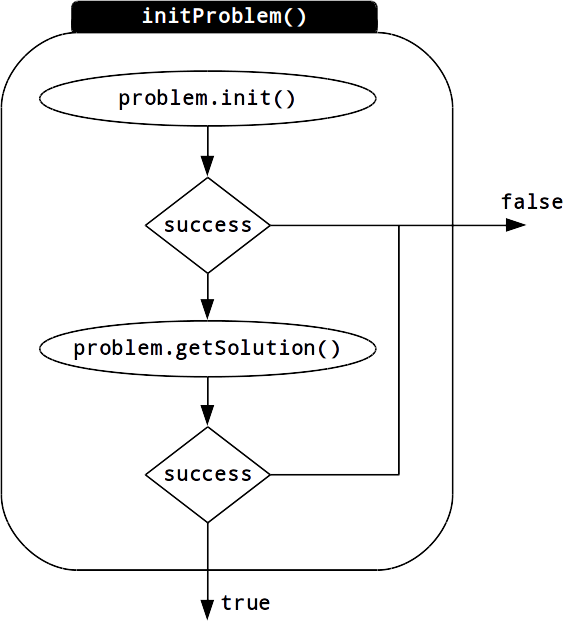
\includegraphics[width=0.3\textwidth]{images/wholebody/QPOasesProblem_init2.png} 
% \caption{The first solution to the IK Problem is given by the \emph{initialization}. After that, \emph{hot-start} and \emph{warm-start} are always attempted to speed-up the computation} 
% \label{qpOasesProblemInit}
% \end{figure}


\subsubsection{Front-End}
The \emph{front-end} prepares all the optimization problems considering the presence of local/global constraints, bounds and priorities. For each task, the cost function is computed as:
\begin{equation}
f(\mathbf{q}_i) = \dot{\mathbf{q}}_i^T\mathbf{J}_i^T\mathbf{W}_i\mathbf{J}_i\dot{\mathbf{q}} + 2(\mathbf{J}_i\dot{\mathbf{q}})^T\mathbf{W}\mathbf{v}_\text{d,i}
\label{cost_function}
\end{equation}
where the second term in (\ref{optimization_problem2}) is automatically added by the solver so the user has only to set the $\lambda$ value. If local constraints are present in the task, they are added to the matrix of the constraints together with the global ones. If the task is not the one at highest priority, the optimality constraints are computed as:
\begin{equation}
\mathbf{J}_{j}\dot{\mathbf{q}}_{j} = \mathbf{J}_{j}\dot{\mathbf{q}}_i
\label{optimality_constraints}
\end{equation}
where $j = 0, 1, ..., i-1$ and $\dot{\mathbf{q}}_{j}$ are the previous computed solutions. The optimality constraints are added together with the other constraints automatically by the \emph{front-end}. Equalities and inequalities constraints are treated together. When the preparation is finished, the solve method of the \emph{back-end} is called (if the QP Problem has been initialized before, otherwise the initialization method is called).

% REMOVED 05/02/16
% \begin{figure}[htb!] 
% \centering 
% 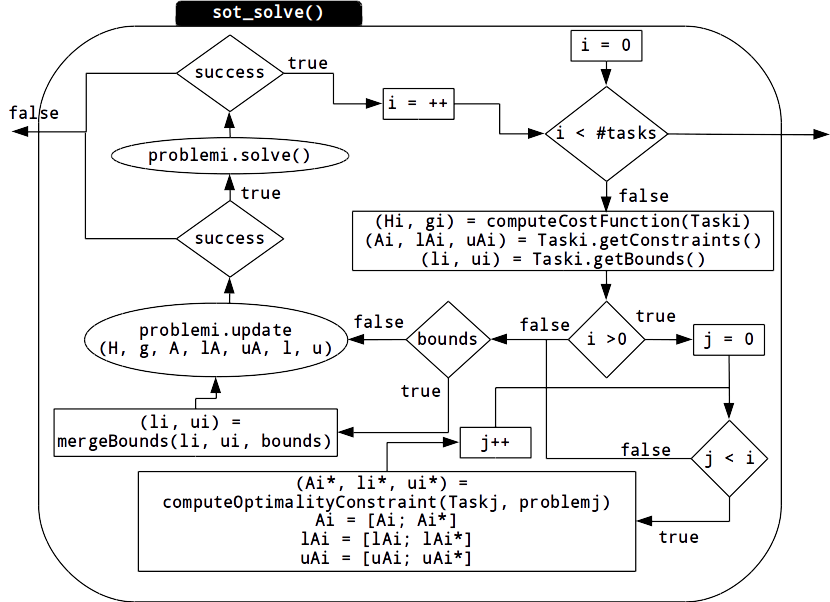
\includegraphics[width=0.6\textwidth]{images/wholebody/QPOases_sot_solve2.png} 
% \caption{The \emph{front-end} is in charge to prepare the IK Problem for the \emph{back-end} writing the QP problems considering priorities, bounds and global/local constraints} 
% \label{qpOasesSoT}
% \end{figure}

Through the \emph{front-end} interface, the user can set parameters regarding each problem in the \emph{back-end}. It is possible to set different options to configure \emph{qpOASES} to favor speed instead of reliability and vice versa. The \emph{front-end} takes care to set default options for \emph{qpOASES}.  

\subsubsection{Considerations on the IK Problem}
It is worth noticing that not only the IK solver but also the IK problem will affect the resulting joint trajectory given by the high-level task solution.
When writing the IK problem, the user may specify different gains and parameters as well as constraints and stacks that will influence in some way the result. From our experience, we used different ways to affect the solution: tuning the $\lambda$ and setting gains for the Cartesian tasks in the cost function of (\ref{optimization_problem2}), add constraints and bounds (however it may result in an unfeasible problem), add a joint space task at the lowest priority level. In the latter case, is well known that when the joint space task is the minimization of the joint velocity, the resulting optimization is equivalent to a weighted pseudo inverse \cite{Siciliano:2008:RMP:1524151}.


\subsection{Experimental Validation}
\label{sec:examples}
In this section we consider a large set of examples and tests to evaluate the performances of the \textbf{OpenSoT} library.

\subsubsection{Soft Interaction and Tele-operation}
\todo{insert paragraph about UI.. or it could go in architecture}\cite{Settimi2014-uo}
For these experiments the \emph{Compliant Inverse Kinematics} scheme has been used as shown in Figure \ref{soft_interaction_block_diagram}.
\begin{figure*}[!h]
\vspace{2 mm}
\centering
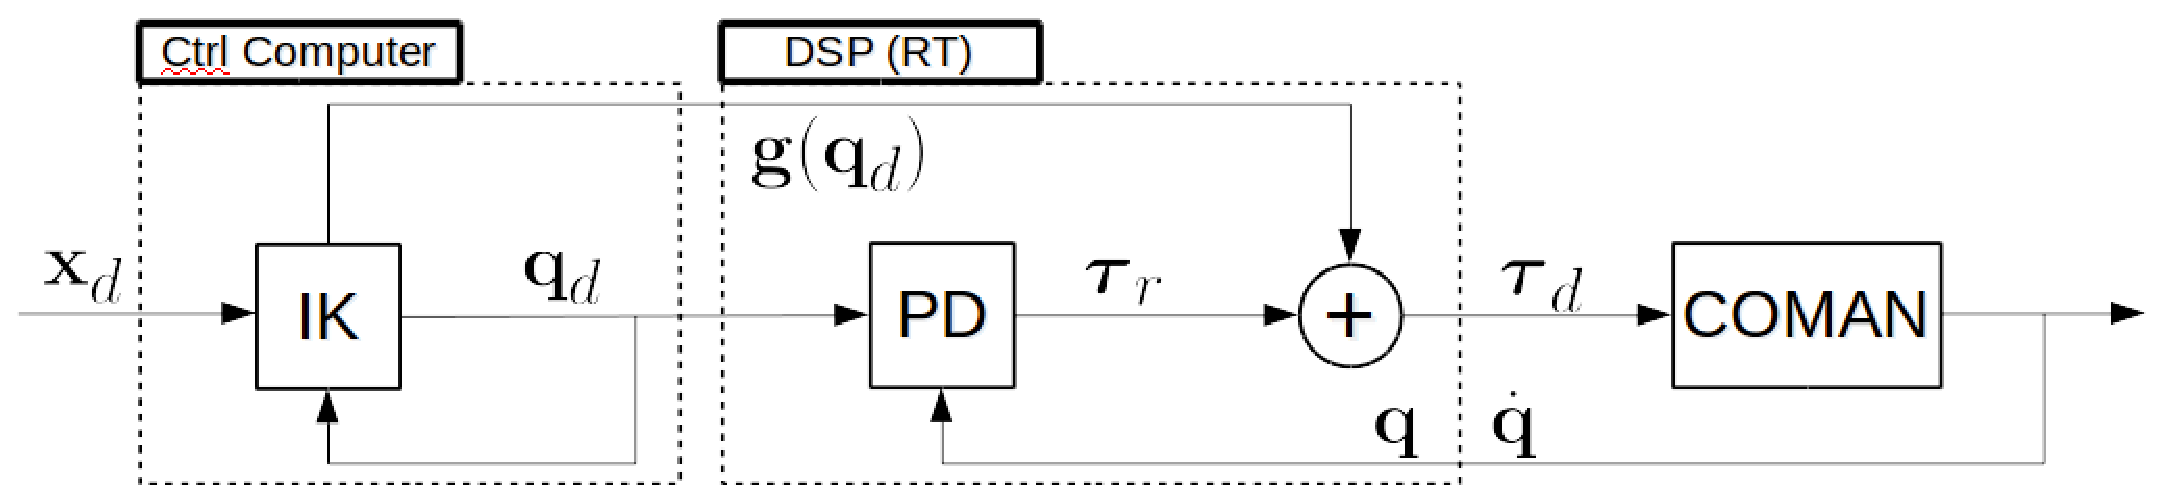
\includegraphics[width=0.6\textwidth]{images/soft_interaction/ctrl_scheme.eps}
\caption{Block diagram for the soft-interactive controller}
\label{soft_interaction_block_diagram}
\end{figure*}
The IK block (\textbf{OpenSoT}) generates joint position references and torques for gravity compensation for the second block that consists in a joint impedance controller. In particular the joint impedance control is implemented in a decentralized way at each DSP in the COMAN robot. The desired torque sent to actuator $i$ is locally computed as
\begin{equation}
    \tau_{d,i} = k_{q,i} (q_{d,i} - q_i) -k_{d,i}\dot{q_i} + g(q_d)_i
    \label{joint_impedance_control}
\end{equation}
where $q_i$ and $q_{d,i}$ are respectively actual and desired joint positions, $\dot{q_i}$ is the  actual joint velocity, $k_{q,i}$ is a positive joint stiffness, $k_{d,i}$ is a positive joint damping and $g(q_d)_i$ is a gravity compensation torque computed at the desired joints configuration.
We consider the following IK problem that is particularly suited for manipulation tasks:
\begin{equation}
\begin{pmatrix}
\left(T_{\substack{\text{Right}\\\text{Wrist}}} + T_{\substack{\text{Left}\\\text{Wrist}}} + T_\text{CoM} + T_{\substack{\text{Right}\\\text{Foot}}}\right) << 
\left(C_{\substack{\text{CoM Velocity}\\\text{Limit}}} + C_{\substack{\text{CoM}\\\text{ConvexHull}}} \right)\setminus\\ 
\\
\left(T_{\substack{\text{Joint}\\\text{Posture}}} + T_{\substack{\text{Minimum}\\\text{Effort}}} \right)
\end{pmatrix}
<< \left(B_{\substack{\text{Joint}\\\text{Limits}}} + B_{\substack{\text{Joint Velocity}\\\text{Limits}}}\right)
\end{equation}
The gain for the Minimum Effort task is $\left( 1 - \beta \right)$ while for the Joint Posture task is $\beta$. The parameter $\beta \in [0, \ 1]$ allows to smoothly on-line weight between a \emph{postural} joint space task to \emph{minimum effort} joint space task. Figure \ref{effort} presents the $2$-norm of the torques in all the 29 joints of the robot. It is easy to recognize the different part where the last task is pure postural ($\beta = 1.0$) and where the last task is pure min effort ($\beta = 0.0$). The difference between the $2$-norm of the torques in pure postural task and in pure min effort task is around $2 [Nm]$ for the given references. 
\begin{figure}
  \centering
    \vspace*{0.05in}
    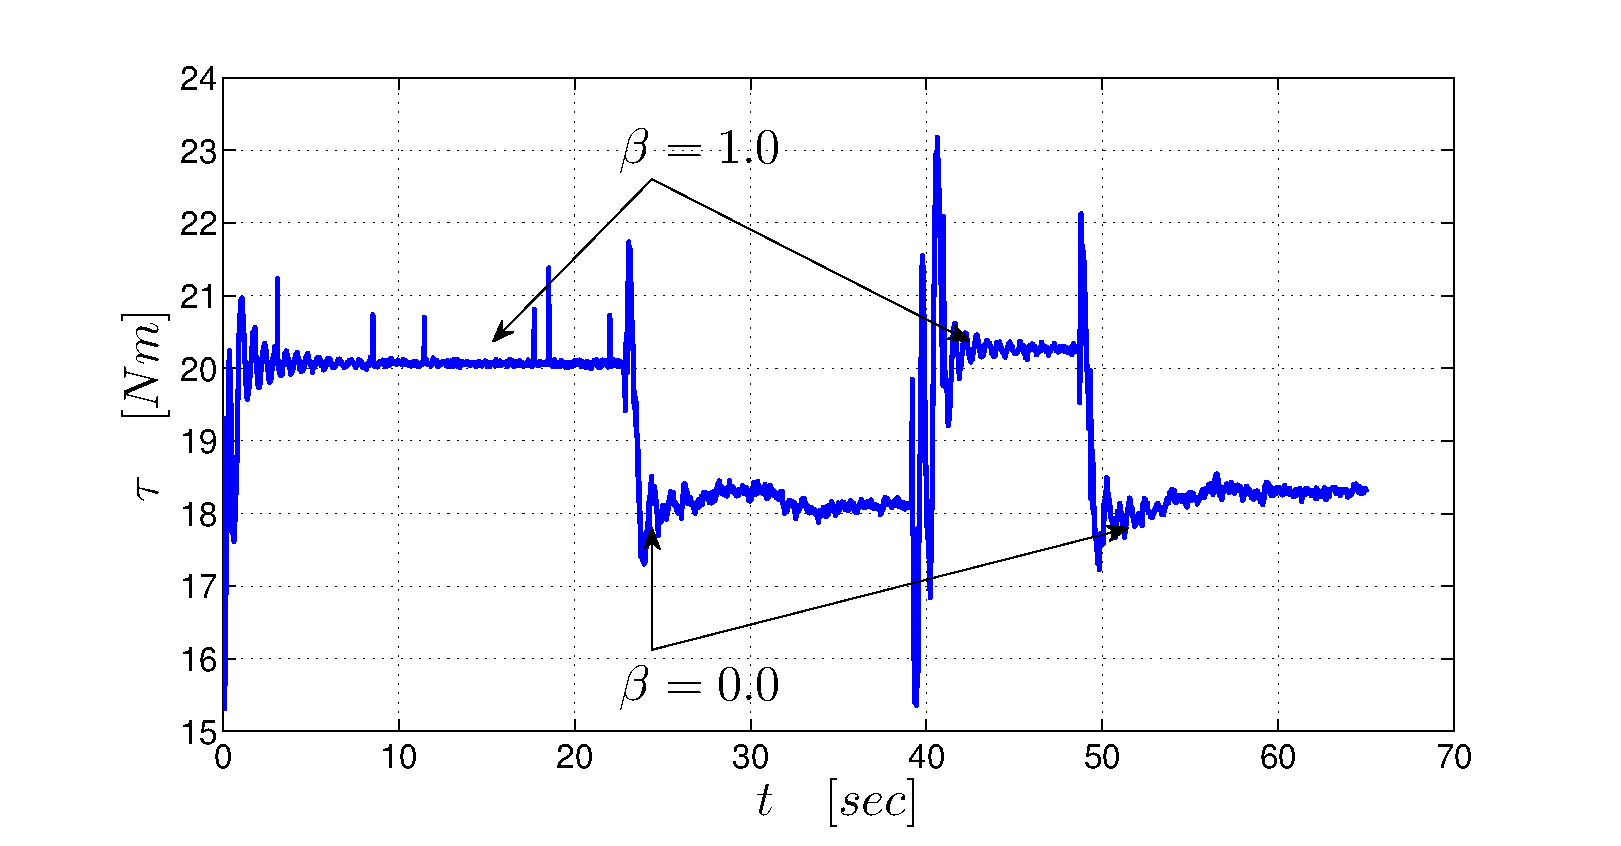
\includegraphics[width=0.7\textwidth]{images/soft_interaction/effort}
    \caption{$2$-norm of torques during switching from a pure postural task to a mix of postural and minimum effort task}\label{effort}
\end{figure} 
The second figure in Figure \ref{CoM_error} depicts the $2$-norm of CoM position error. The error for a certain kinematic chain is computed as the sum of the $2$-norms of the Cartesian error between the desired and computed Cartesian pose.
\begin{figure}
    \centering
    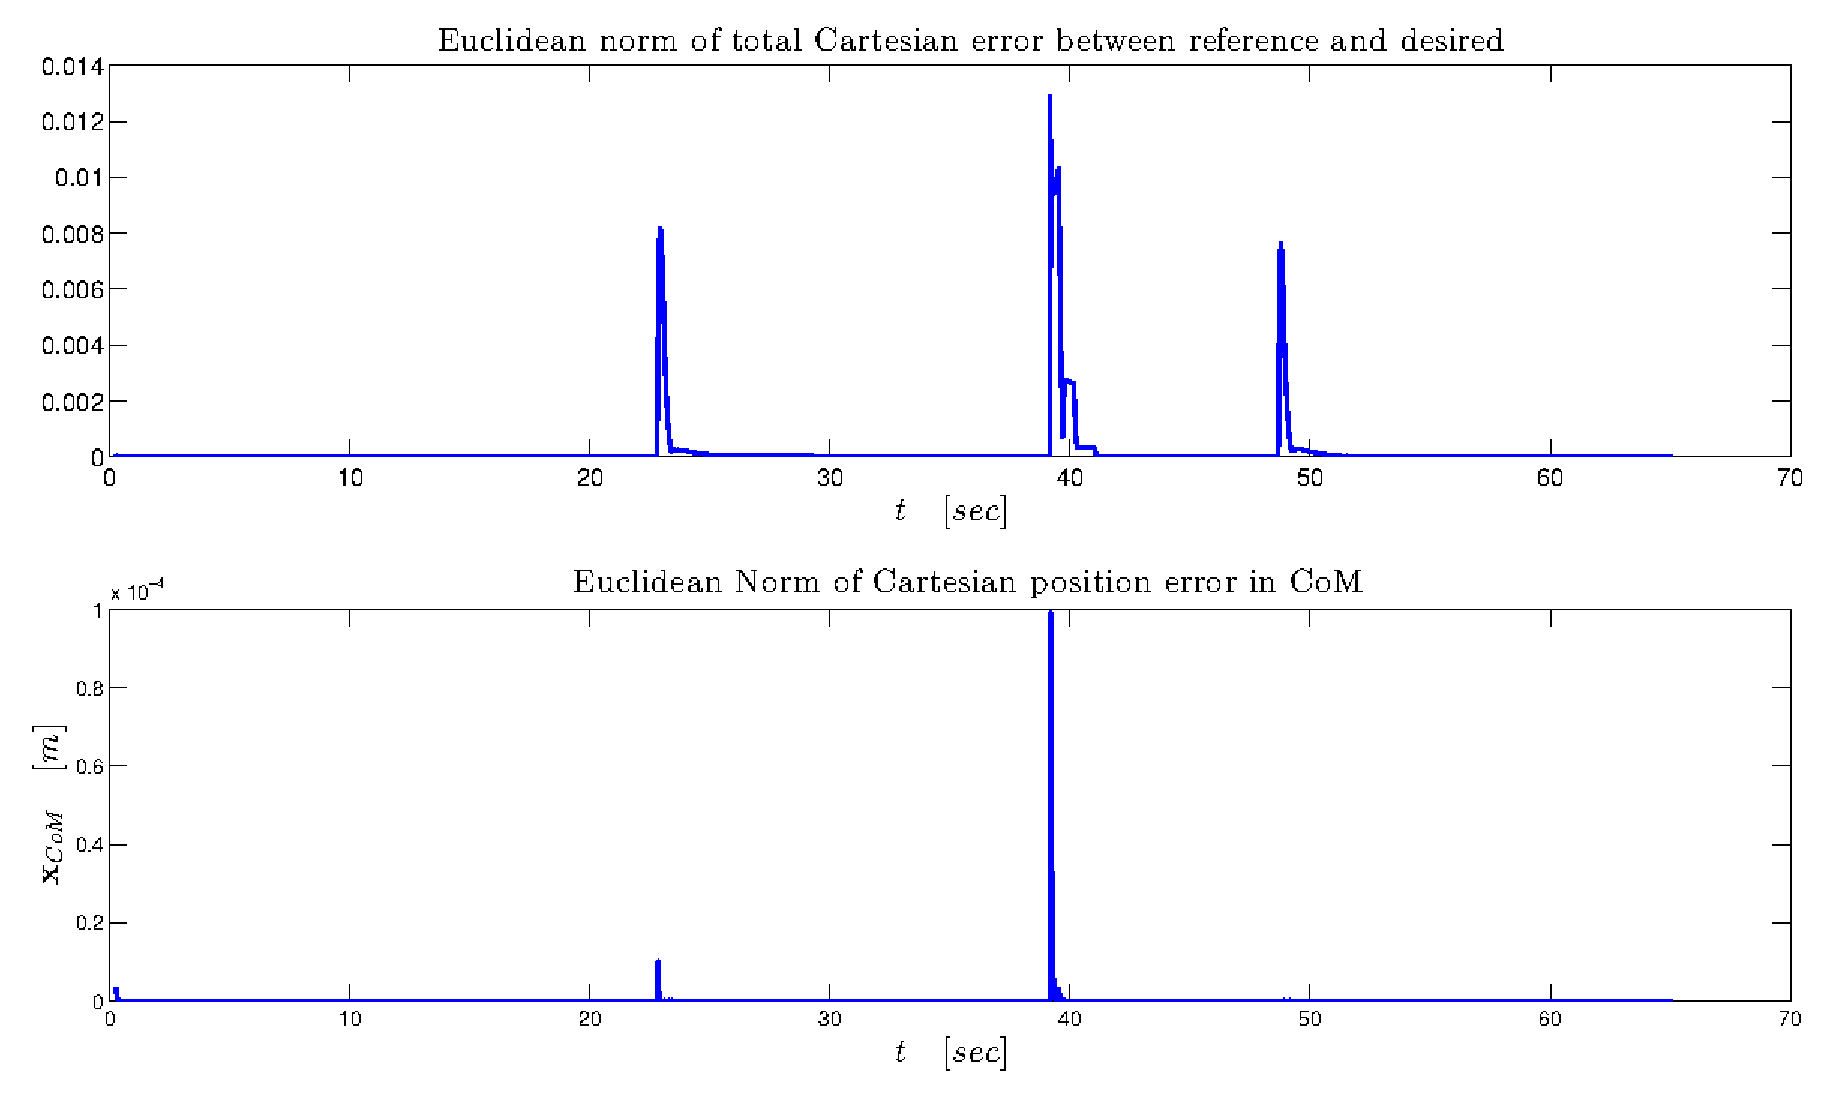
\includegraphics[width=0.7\textwidth]{images/soft_interaction/CartesianErrors}
    \caption{$2$-norm of Cartesian errors for CoM and end effectors}\label{CoM_error}
\end{figure}
It can been seen that the CoM is adequately maintained with the predefined reference position even during the switching of the tasks. 
Error in joint trajectory generation increases only during switching phases. The $2$-norm of the vector of the joint errors is presented in the first figure in Figure \ref{CoM_error}.
Finally in Figure \ref{COMAN_exp} the COMAN is shown in different postures arising by changing $\beta$ in the secondary task, the COMAN kinematic structure consists in 6 DoFs legs, 7 DoFs arms and a 3 DoFs torso.
\begin{figure}
        \centering
        \vspace{2mm}
        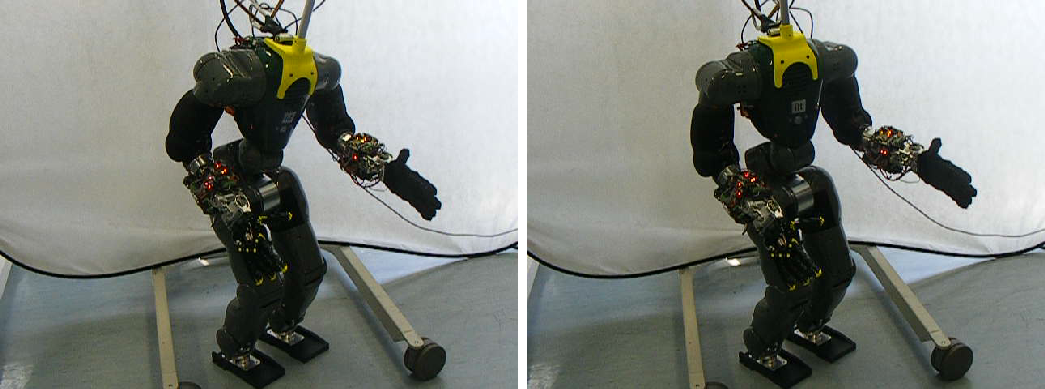
\includegraphics[width=0.7\textwidth]{images/soft_interaction/postural_min_effort.png}
        \caption{COMAN holding end-effectors pose while executing a postural task (left) or a minimum effort task (right)}
        \label{COMAN_exp}
\end{figure}
This particular IK problem and low-level controller have been also used to perform tasks with high level of interaction with the environment such as a writing task, Figure \ref{COMAN_love}, a cleaning task, Figure \ref{COMAN_bb} and a handover task, Figure \ref{COMAN_handover}. The joint impedance control makes the interaction possible and safe reducing impact/contact forces that may compromise the robot stability, damage the robot itself or the environment. The whole-body IK runs in open loop to prevent the action of the feedback during interaction from counteracting the effect of compliant behavior.

\begin{comment}
\begin{figure}
        \centering
        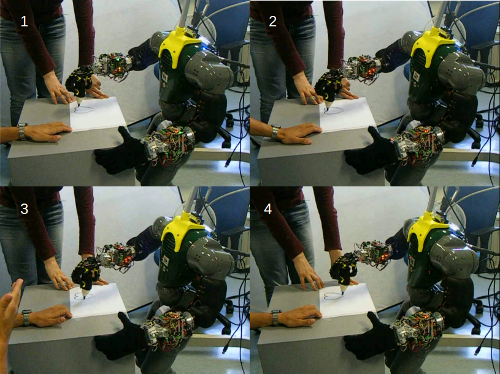
\includegraphics[width=0.7\textwidth]{images/soft_interaction/sot_love.png}
        \caption{COMAN performing a drawing task on a desk, interaction is handled by joint impedance control}
        \label{COMAN_love}
\end{figure}
\end{comment}

\begin{comment}
\begin{figure}
        \centering
        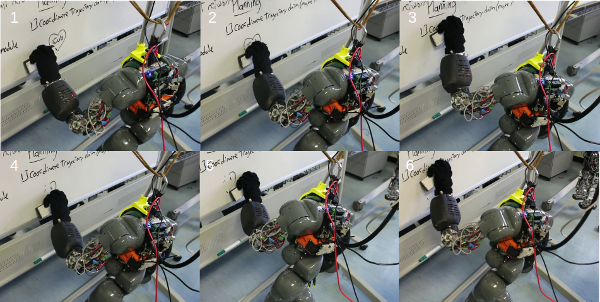
\includegraphics[width=0.7\textwidth]{images/soft_interaction/sot_bb.png}
        \caption{COMAN erasing a whiteboard, interaction is handled by the joint impedance control}
        \label{COMAN_bb}
\end{figure}

\begin{figure}
        \centering
        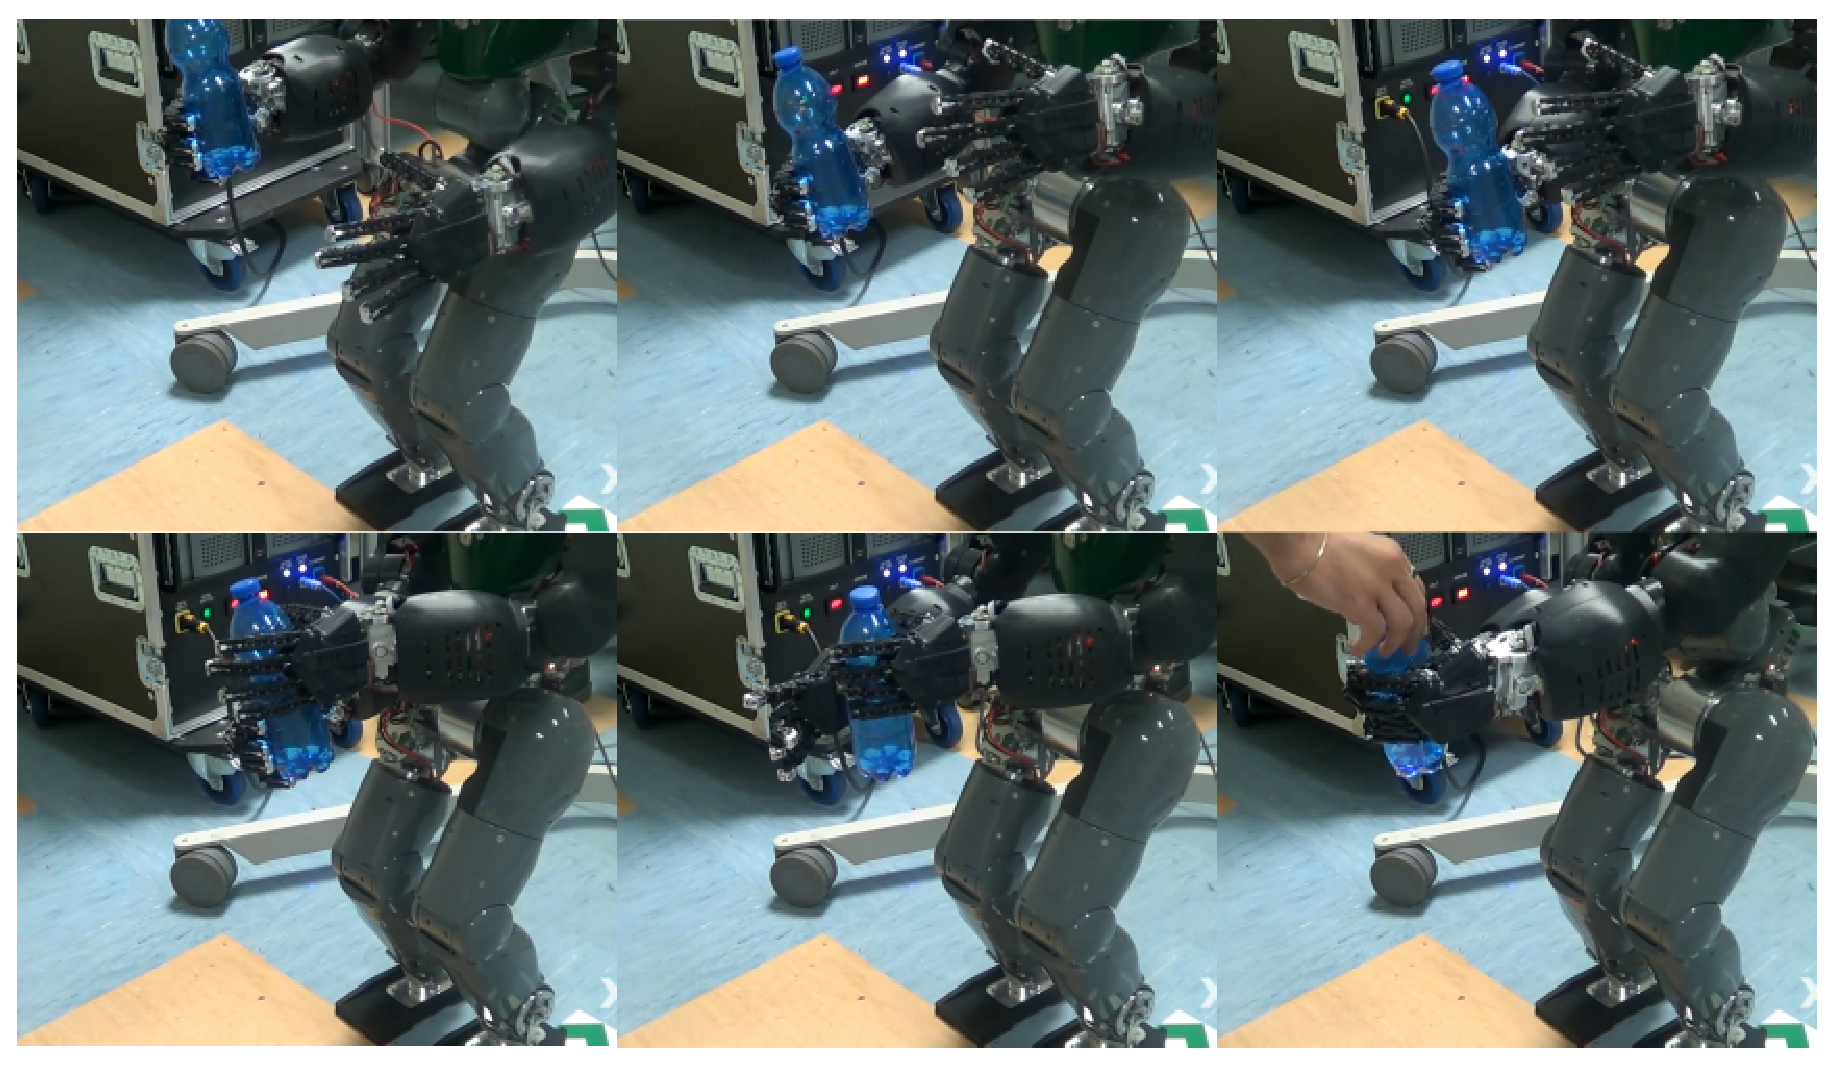
\includegraphics[width=0.7\textwidth]{images/soft_interaction/handover.eps}
        \caption{COMAN performing an handover task}
        \label{COMAN_handover}
\end{figure}
\end{comment}

\begin{figure}
% \centering
% \begin{minipage}[b]{7.7cm}
        \centering
        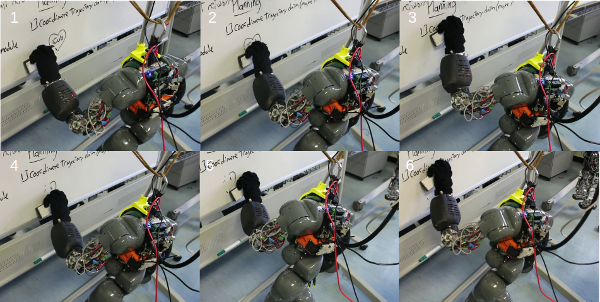
\includegraphics[width=1.0\textwidth]{images/soft_interaction/sot_bb.png}
        \caption{COMAN erasing a whiteboard, interaction is handled by the joint impedance control}
        \label{COMAN_bb}
% \end{minipage}
%  \ \hspace{3mm} \
% \begin{minipage}[b]{7.7cm}
%         \centering
%         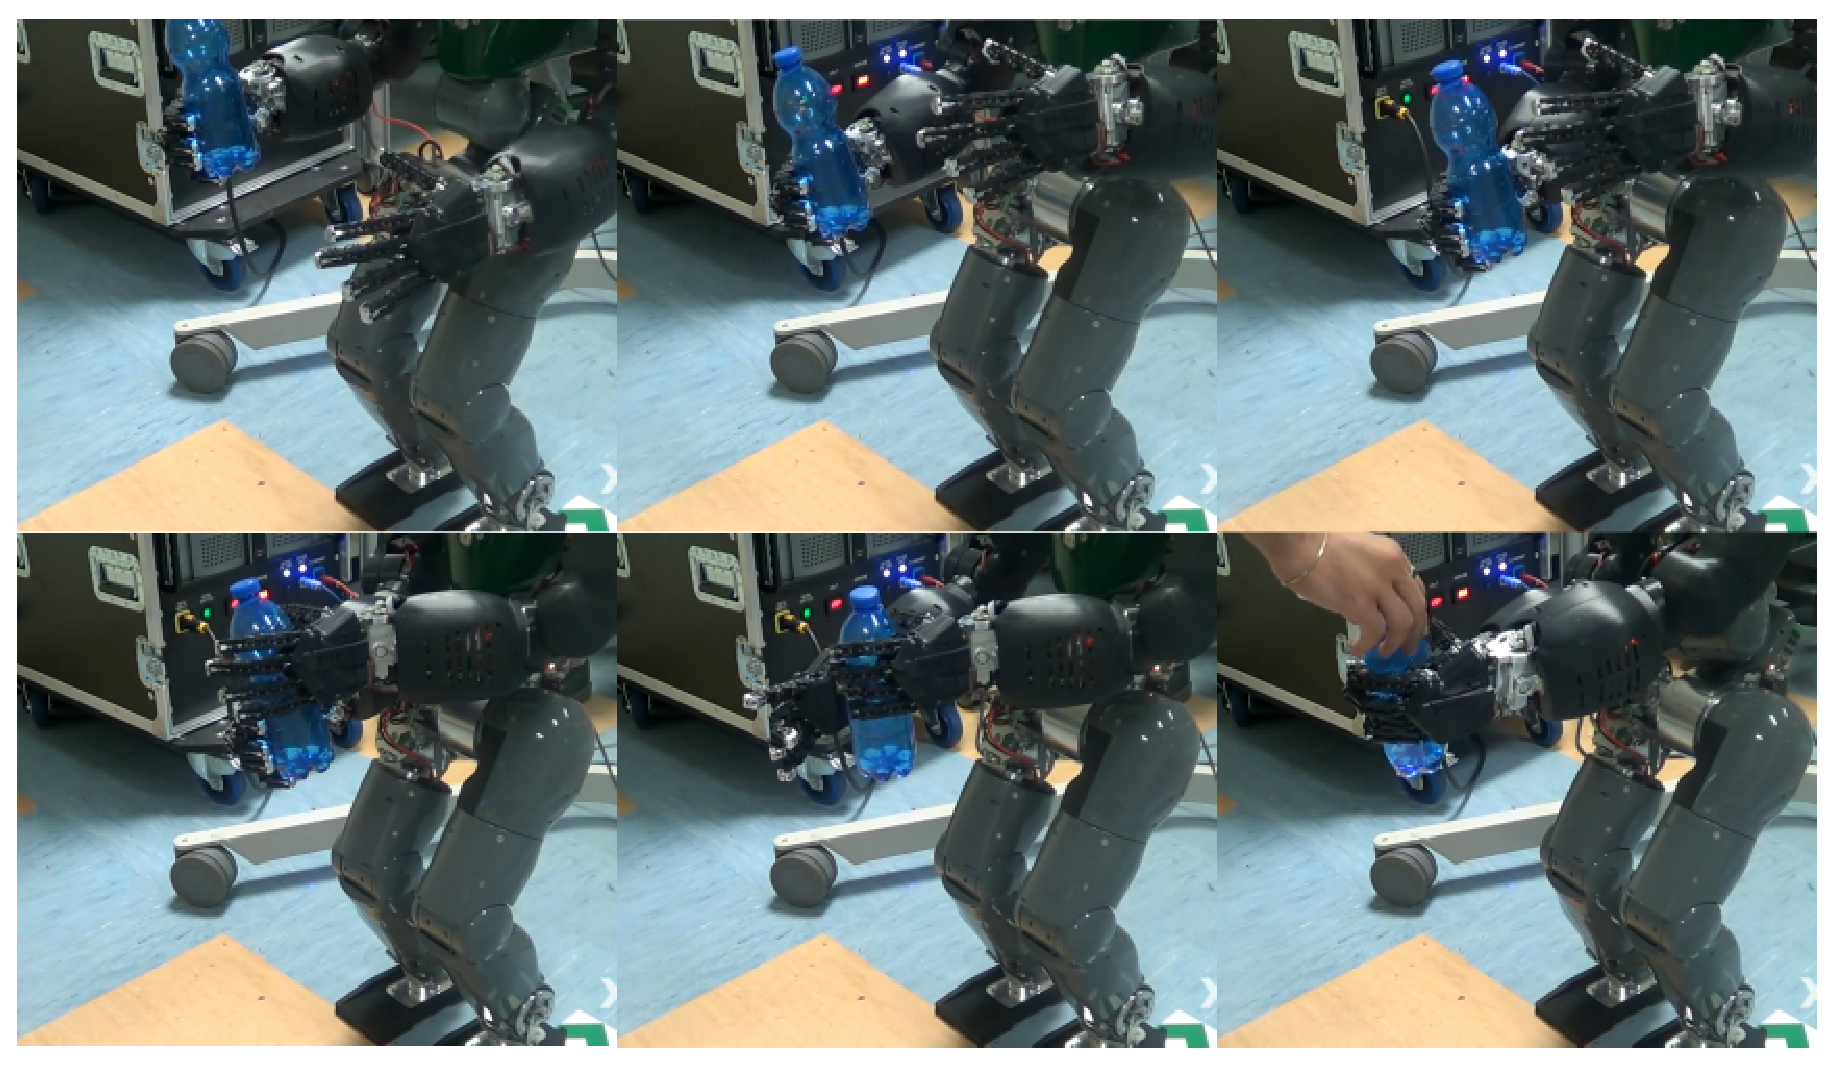
\includegraphics[width=1.0\textwidth]{images/soft_interaction/handover.eps}
%         \caption{COMAN performing an handover task}
%         \label{COMAN_handover}
% \end{minipage}
\end{figure}

\begin{comment}
\begin{figure}
        \centering
        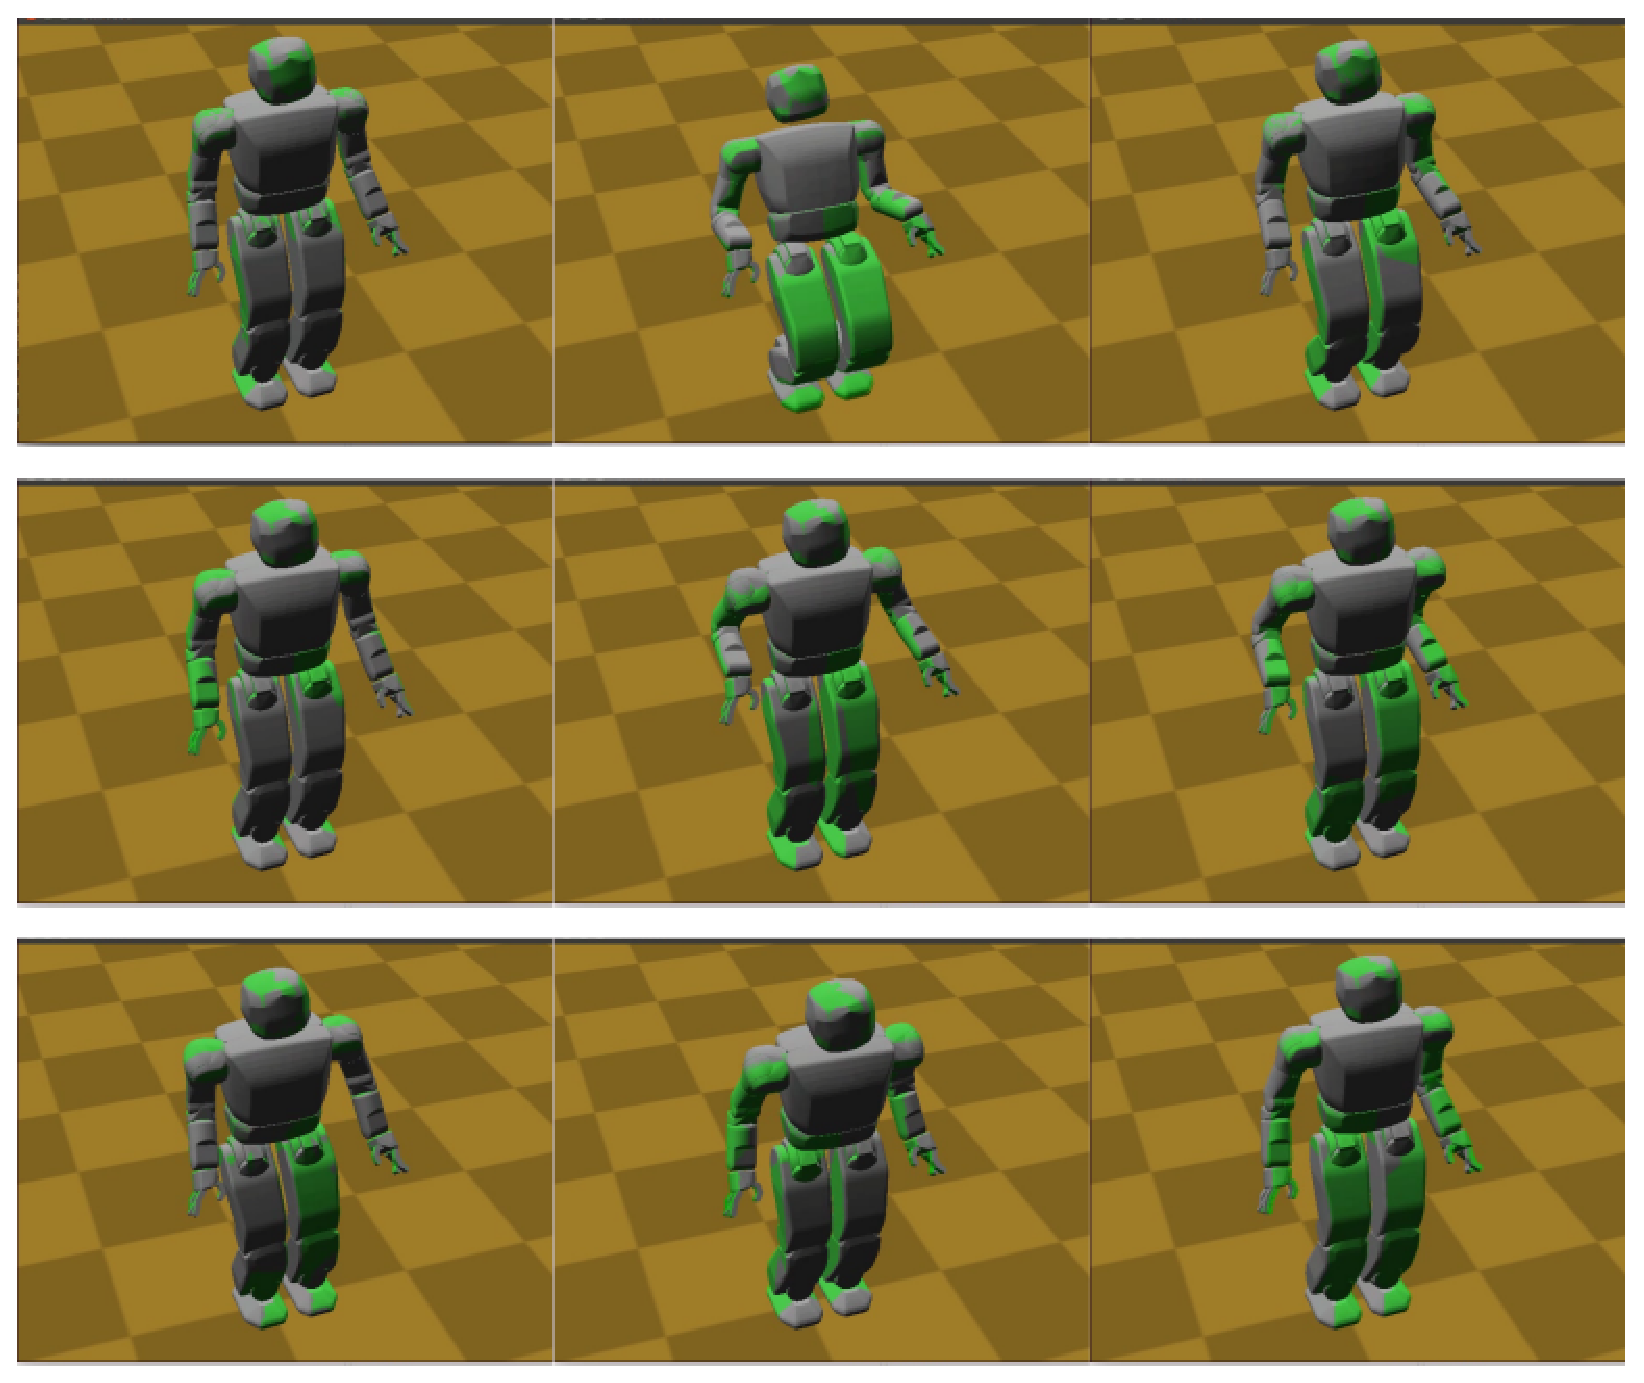
\includegraphics[width=0.7\textwidth]{images/soft_interaction/hubo.eps}
        \caption{HUBO performing whole-body tasks: from top to bottom, squat, arm trajectories (circle on left wrist, up-down with right wrist) and circular CoM trajectories on the x-y plane respectively. The stack for the three task is a whole body stack composed of \texttt{stack = ((r\_leg+l\_leg)/CoM\_XY/(waist\_Z)/(l\_arm+r\_arm)/postural) << j\_lims << j\_vel\_lims; velocityAllocation(stack,0.3,0.6,1.0)}. The Hubo robot used in the simulation has a $1$ DoFs torso, $6$ DoFs legs and arms, $2$ DoFs neck, $15$ DoFs arms}
        \label{fig:HUBO}
\end{figure}
\end{comment}

\begin{figure}
\begin{minipage}[b]{7.7cm}
        \centering
        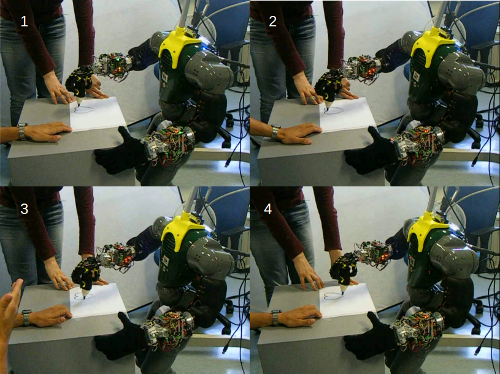
\includegraphics[width=1.0\textwidth]{images/soft_interaction/sot_love.png}
        \vspace{1mm}
        \caption{COMAN performing a drawing task on a desk, interaction is handled by joint impedance control\vspace{5mm}}
        \label{COMAN_love}
\end{minipage}
 \ \hspace{3mm} \
\begin{minipage}[b]{7.7cm}
        \centering
        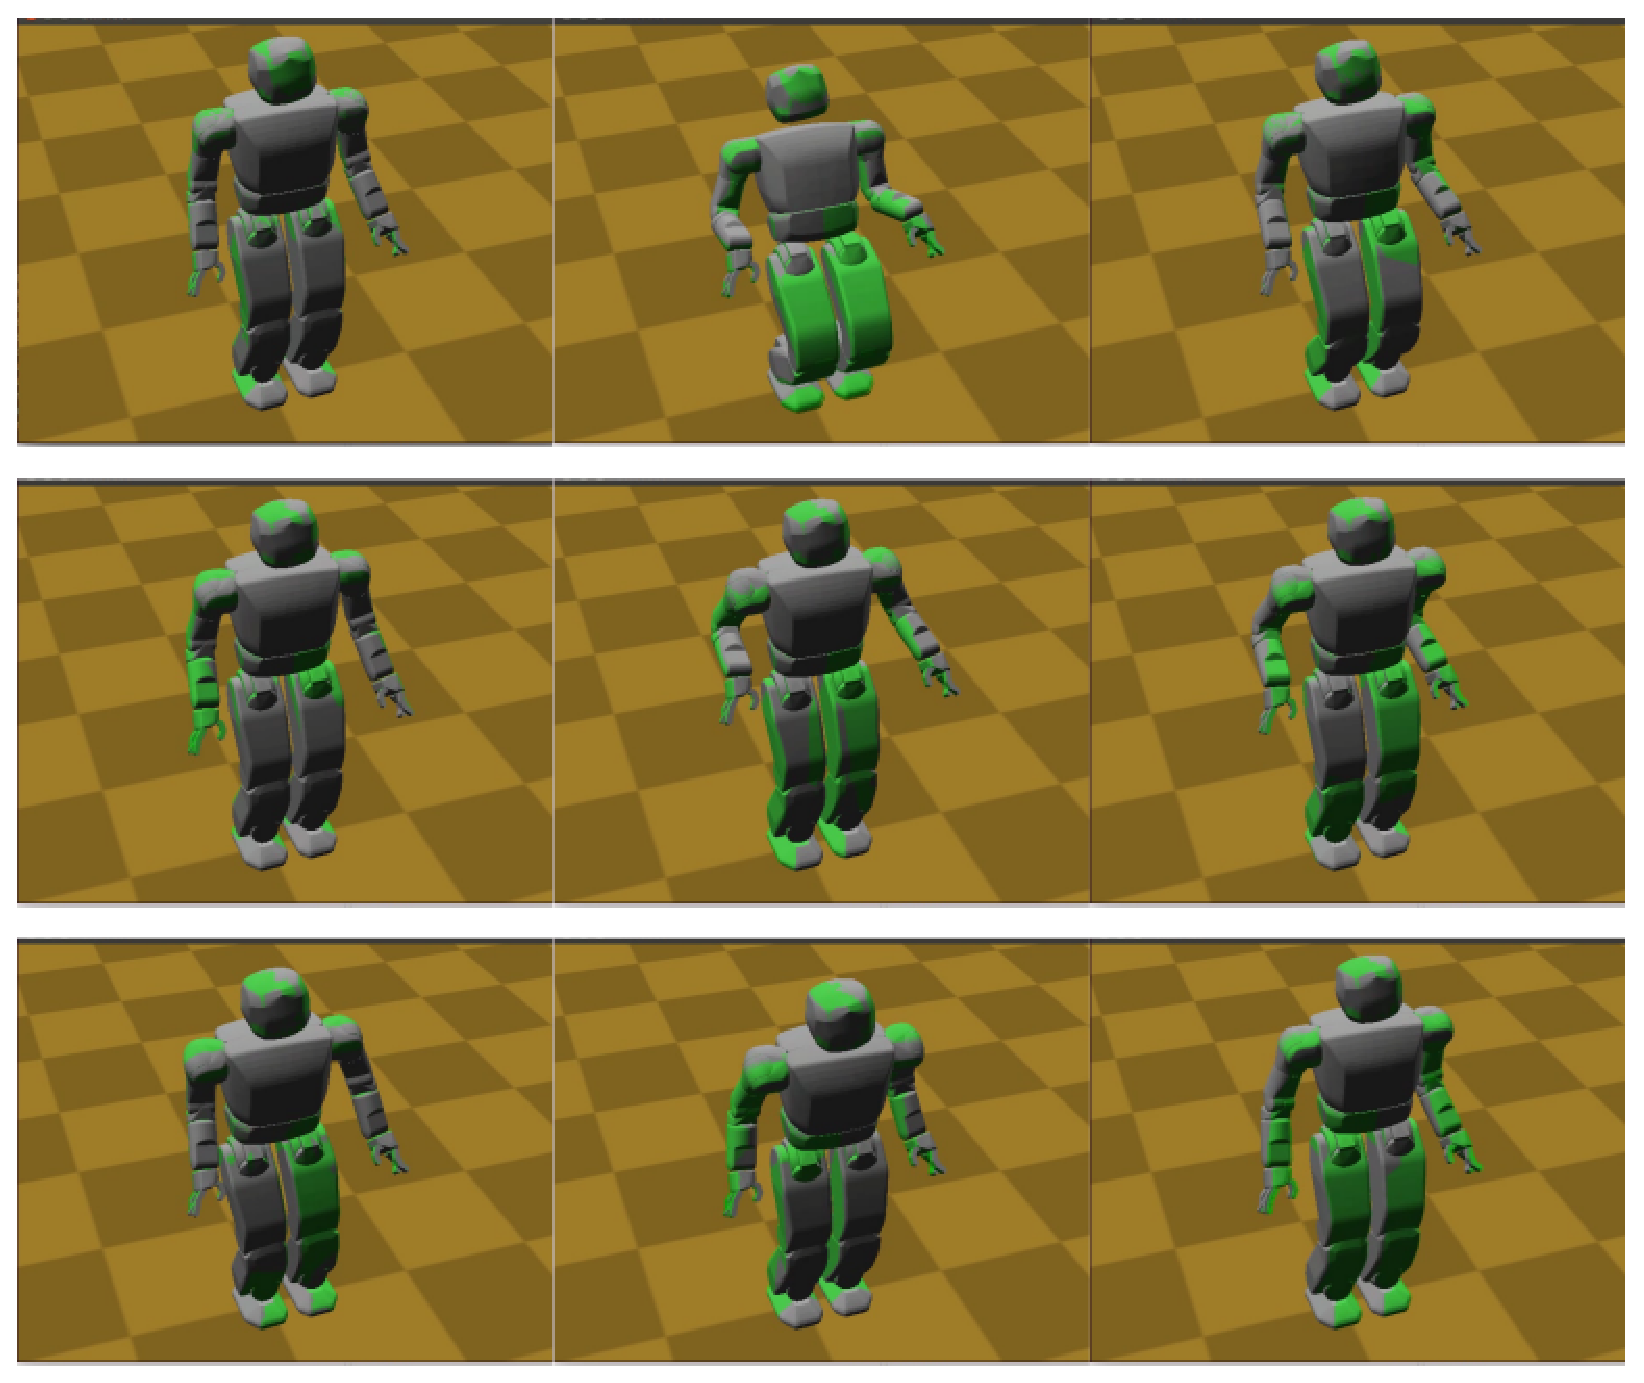
\includegraphics[width=1.0\textwidth]{images/soft_interaction/hubo.eps}
        \caption{HUBO performing whole-body tasks: from top to bottom, squat, arm trajectories (circle on left wrist, up-down with right wrist) and circular CoM trajectories on the x-y plane respectively}
        \label{fig:HUBO}
\end{minipage}
\end{figure}

% REMOVED 05/02/16
% \subsubsection{Locomotion}
% In this experiment, two IK problems are compared to perform a walking task while moving an arm using the simulated model of WALK-MAN (the kinematics of WALK-MAN consists in 6 DoFs legs, 7 DoFs arms, 3 DoFs torso and 2 DoFs neck). The block diagram is shown in Figure \ref{walk_block_diagram}.
% \begin{figure*}[!h]
% \vspace{2 mm}
% \centering
% 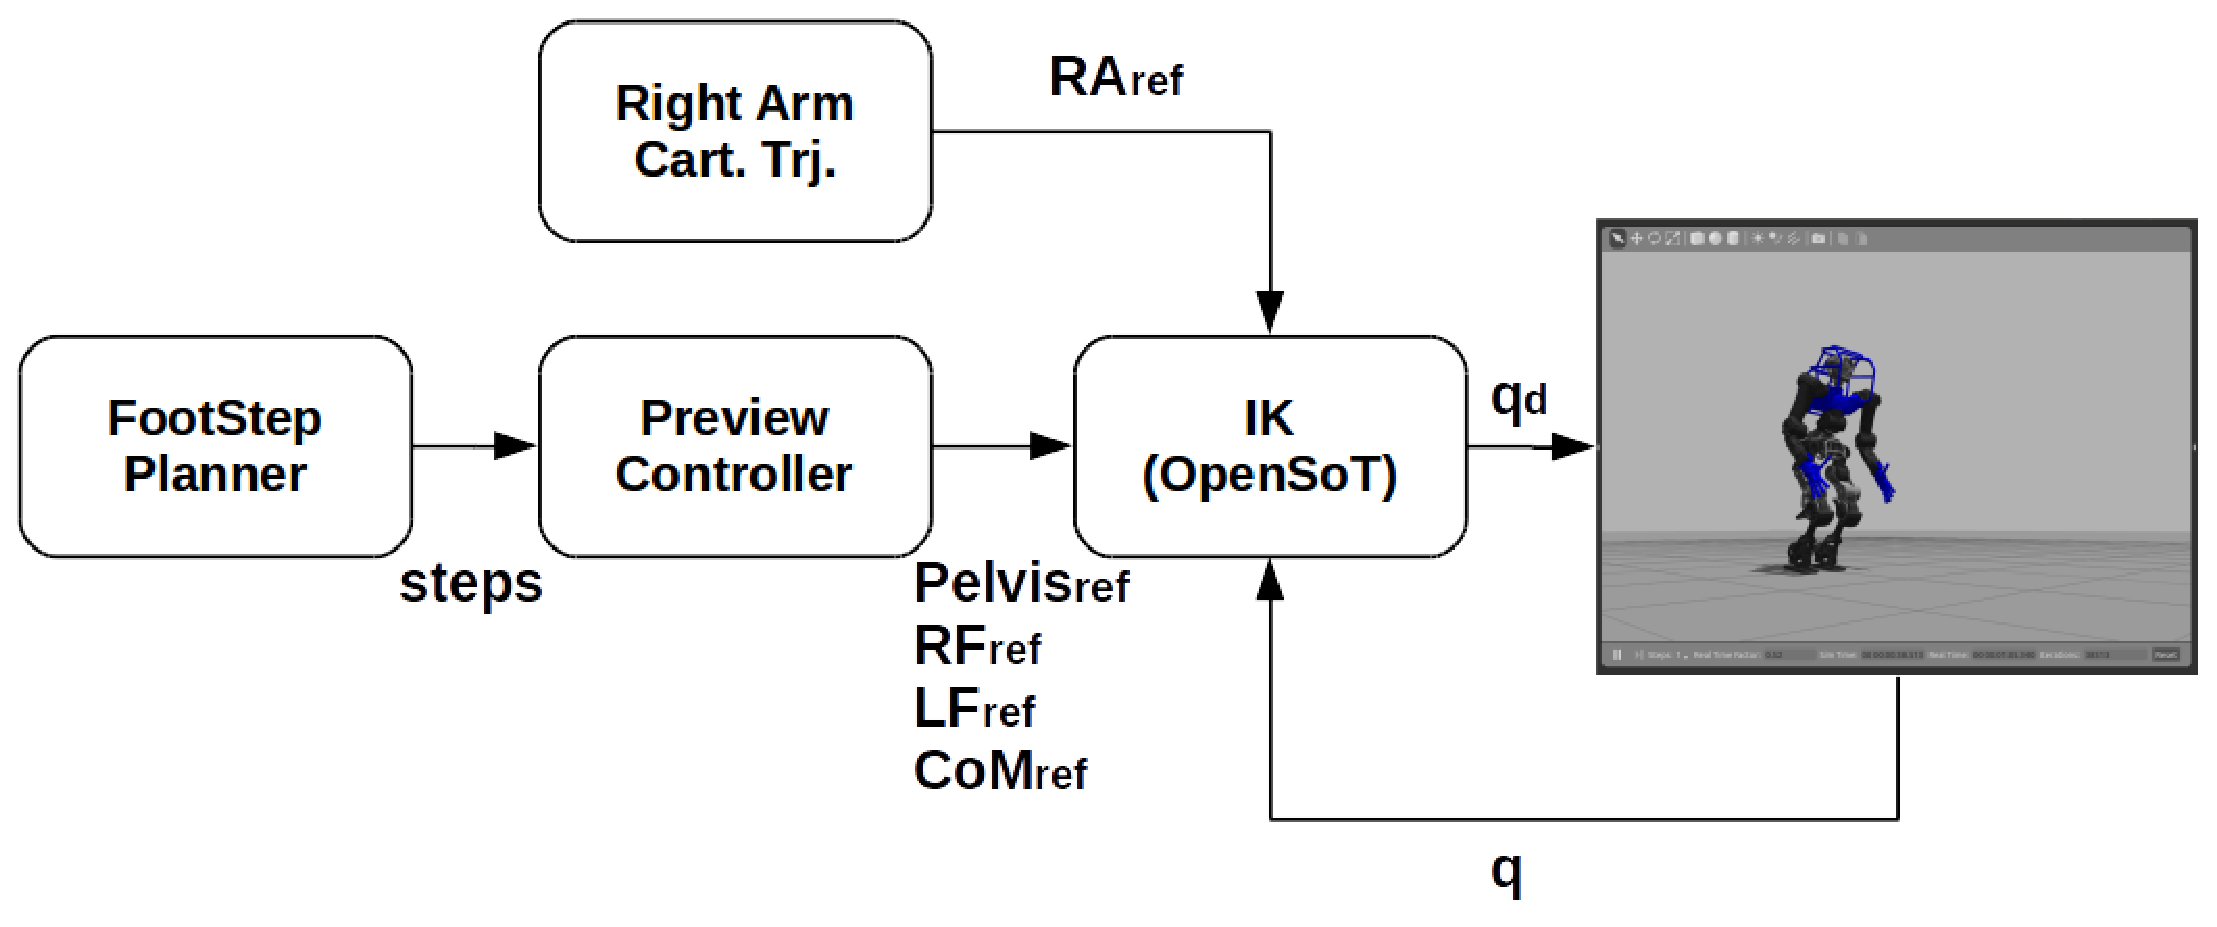
\includegraphics[width=0.8\textwidth]{images/walking/walking.eps}
% \caption{Block diagram for the walking task with WALK-MAN}
% \label{walk_block_diagram}
% \end{figure*}
% It is worth to notice that no additional stabilizers are used after the \emph{Preview Controller} \cite{Kajita:03}.
% From a foot-step planner, a set of step is computed. These steps are the input for the \emph{Preview Controller} that computes Cartesian trajectories for the CoM considering a stable trajectory for the Zero Moment Point (ZMP) and an Inverted Pendulum Model as well as Cartesian trajectories for the feet. Most of the time, researchers suppose the upper body does not move at all while walking and they control the pelvis instead of the CoM. Indeed, the \emph{Preview Controller} assumes the whole robot represented as its CoM and a leg on the ground. In this experiment the right arm is moved while walking and this movement is not taken into account when generating the trajectories from the \emph{Preview Controller}. To have a stable walking the CoM control is needed since it will compensate for the CoM displacement generated by the arm movements. Controlling just the pelvis generate an unstable walking.
% The IK Problems considered are:
% \begin{equation}
% \begin{pmatrix}
% \left(T_{\substack{\text{Right}\\\text{Foot}}} + T_{\substack{\text{Left}\\\text{Foot}}} + T_\text{Pelvis}\right)\setminus\\
% \\
% T_{\substack{\text{Right}\\\text{Wrist}}}\setminus\\
% \\
% T_{\substack{\text{Joint}\\\text{Posture}}}
% \end{pmatrix}
% << \left(B_{\substack{\text{Joint}\\\text{Limits}}} + B_{\substack{\text{Joint Velocity}\\\text{Limits}}}\right)
% \end{equation}
% and
% \begin{equation}
% \begin{pmatrix}
% \left(T_{\substack{\text{Right}\\\text{Foot}}} + T_{\substack{\text{Left}\\\text{Foot}}} + T_\text{CoM}\right)\setminus\\
% \\
% T_{\substack{\text{Right}\\\text{Wrist}}}\setminus\\
% \\
% T_{\substack{\text{Joint}\\\text{Posture}}}
% \end{pmatrix}
% << \left(B_{\substack{\text{Joint}\\\text{Limits}}} + B_{\substack{\text{Joint Velocity}\\\text{Limits}}}\right)
% \end{equation}
% In Figure \ref{walk_snapshot}, the results of the two controllers is shown. On the left, the pelvis is controlled and the continuous movement of the arm makes the robot fall. On the right the CoM is controlled and the robot can use the whole body to compensate for the arm movement. 
% \begin{figure*}[!h]
% \vspace{2 mm}
% \centering
% \includegraphics[width=\textwidth]{images/walking/walking_snapshot.eps}
% \caption{Walking performances of the two IK Problems}
% \label{walk_snapshot}
% \end{figure*}


\subsubsection{Examples}
In this part we focus on a set of tasks and constraints that have been used in practice in a series of stacks of practical interest. The experiments show their behaviour and performances.

\paragraph{Dynamic Filter}
As explained before, the idea behind the \emph{Dynamic Filter} is to use the dynamics of the robot to filter non-feasible motions. In this experiment the effect of the dynamics as a constraint, at the velocity level, is shown. The robot has to perform a squat motion that requires a certain amount of torque on the legs. The same motion is then performed with the constraints considering that the available torque at the legs is $60\%$  less ($20 \ [Nm]$ instead of $50 \ [Nm]$). 
The IK Problems considered is:
\begin{equation}
\begin{pmatrix}
T_{\substack{\text{Right}\\\text{Foot}}}\setminus\\
\\
\left(T_{\substack{\text{Right}\\\text{Wrist}}} + T_{\substack{\text{Left}\\\text{Wrist}}} + T_\text{Waist} + T_\text{Torso} + T_\text{CoM}\right)\setminus\\ 
\\
T_{\substack{\text{Joint}\\\text{Posture}}}
\end{pmatrix}
<< \left(B_{\substack{\text{Joint}\\\text{Limits}}} + B_{\substack{\text{Joint Velocity}\\\text{Limits}}} + C_\text{Dyn}\right)
\end{equation}

\begin{figure*}[!h]
\vspace{2 mm}
\centering
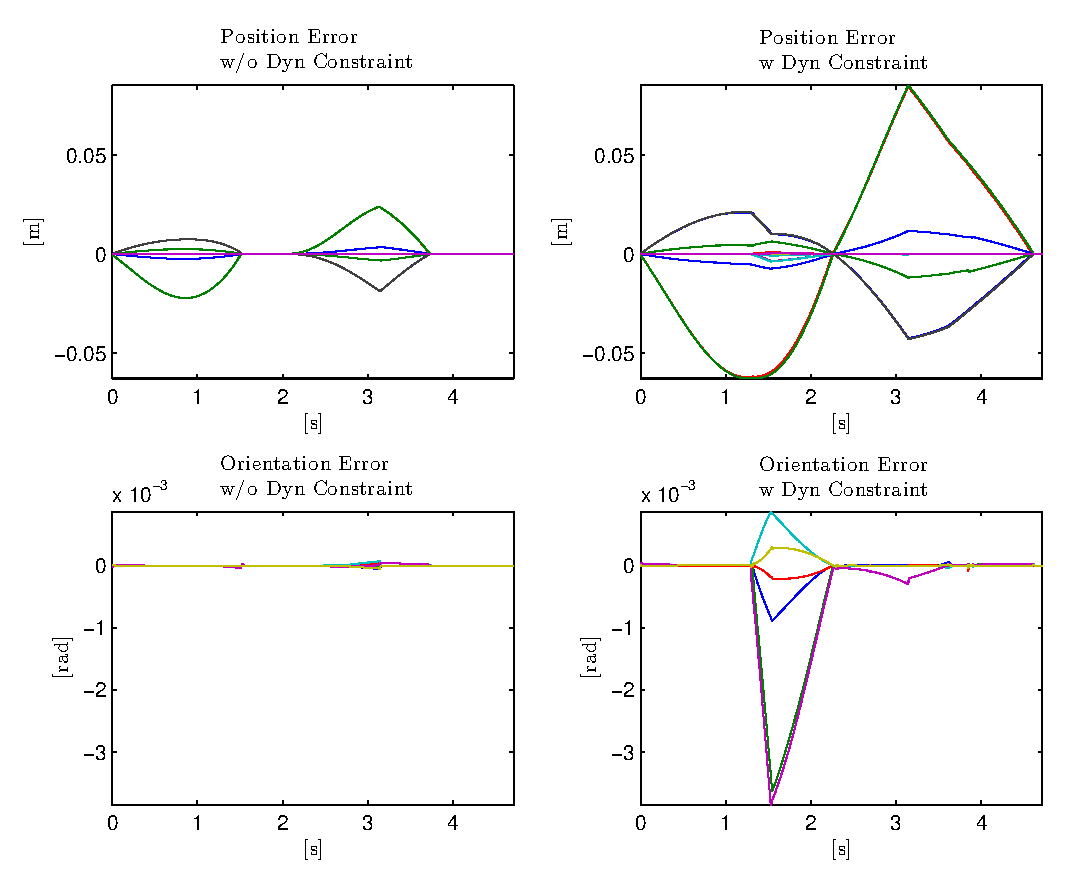
\includegraphics[width=0.8\textwidth]{images/dyn/Cartesian_error_dyn.eps}
\caption{Cartesian errors during squat motion. On the left w/o Dynamic constraint, on the right w Dynamic constraint}
\label{cartesian_error_dyn}
\end{figure*}
In Figure \ref{tau_dyn} is possible to see the effect of the Dynamic constraint: some of the torques (on the legs) exceed the threshold of $20 \ [Nm]$ when not using the constraint while, in the other case, all the torques are in the bounds. In Figure \ref{dq_dyn}, also the computed velocity are smooth wrt the one computed without the constraint. This is payed in terms of Cartesian error, in Figure \ref{cartesian_error_dyn} is clear that the more aggressive control (without the Dynamic constraint) can track better the reference. Figure \ref{motion_dyn_constr} shows the generated motions in the two cases.

\begin{figure*}
    \vspace{2 mm}
    \centering
        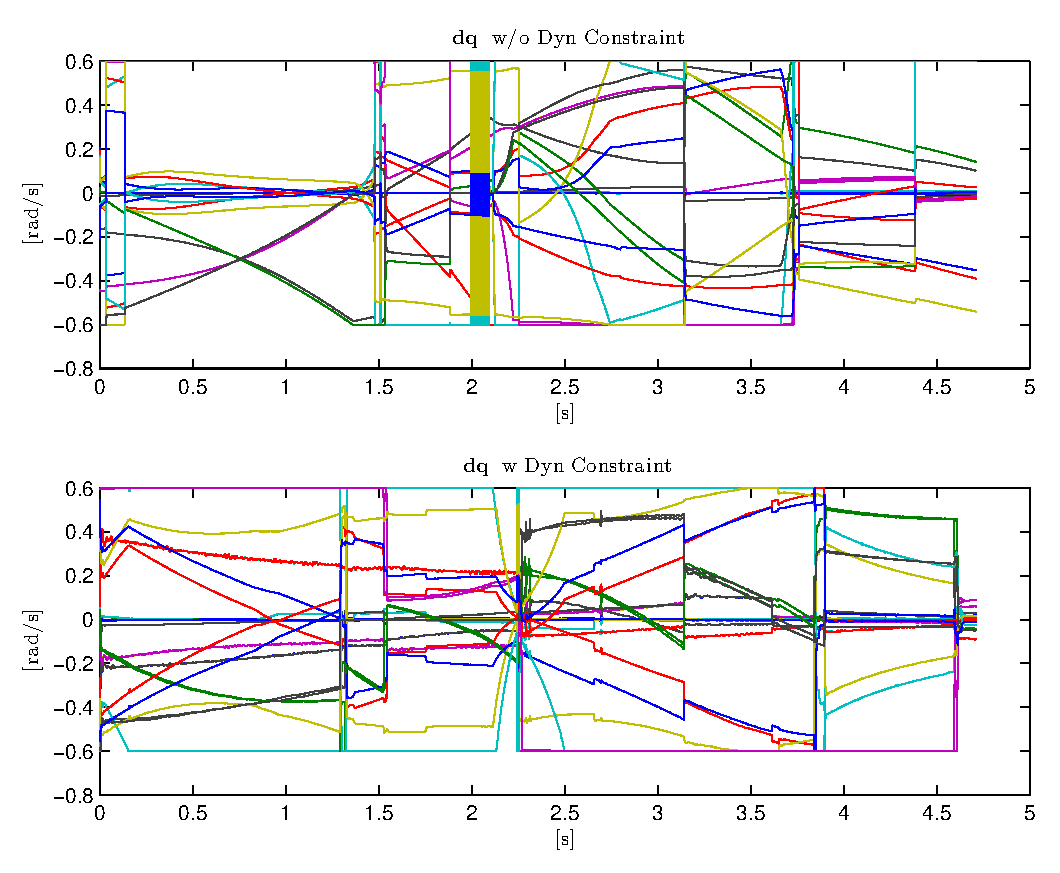
\includegraphics[width=0.7\textwidth]{images/dyn/dq_dyn.eps} 
        \caption{Computed joint velocities}
        \label{dq_dyn}
\end{figure*}

\begin{figure*}
    \vspace{2 mm}
    \centering
        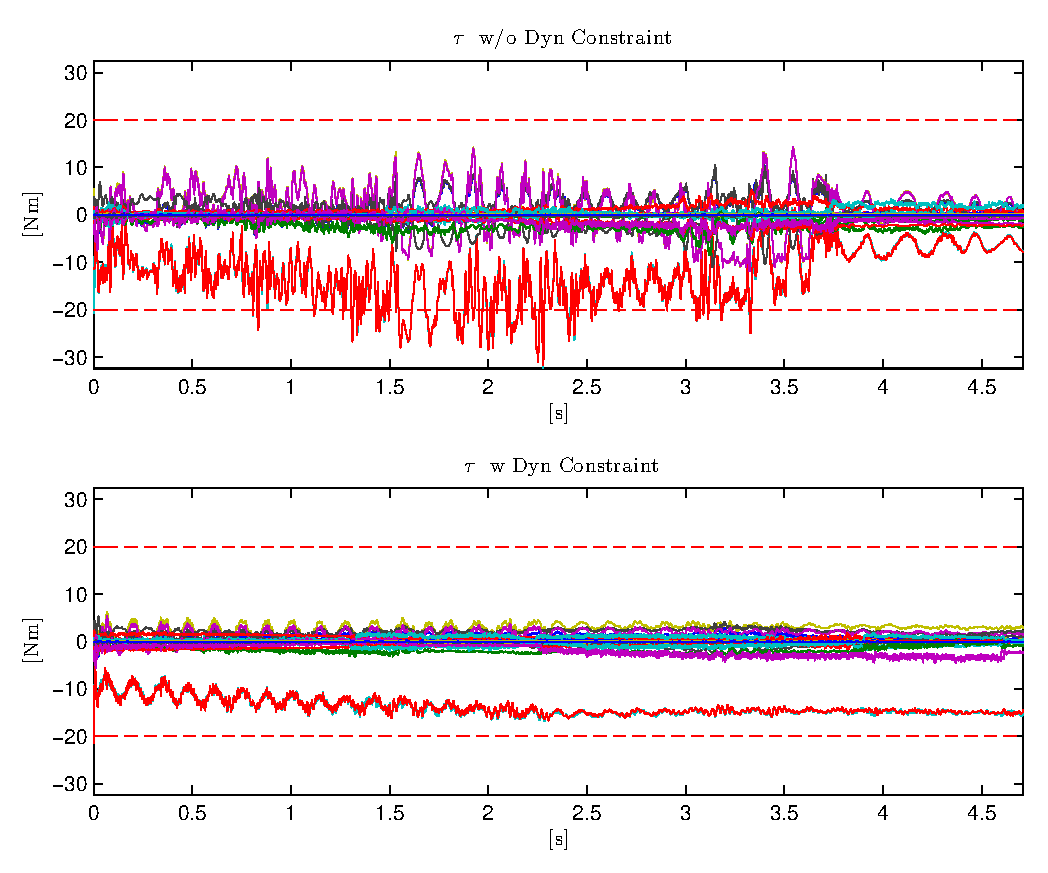
\includegraphics[width=0.7\textwidth]{images/dyn/tau_dyn.eps}
        \caption{Computed joint torques}
        \label{tau_dyn}
\end{figure*}

%\begin{sidewaysfigure}
%    \centering
    %\begin{subfigure}[b]{0.8\textwidth}
%        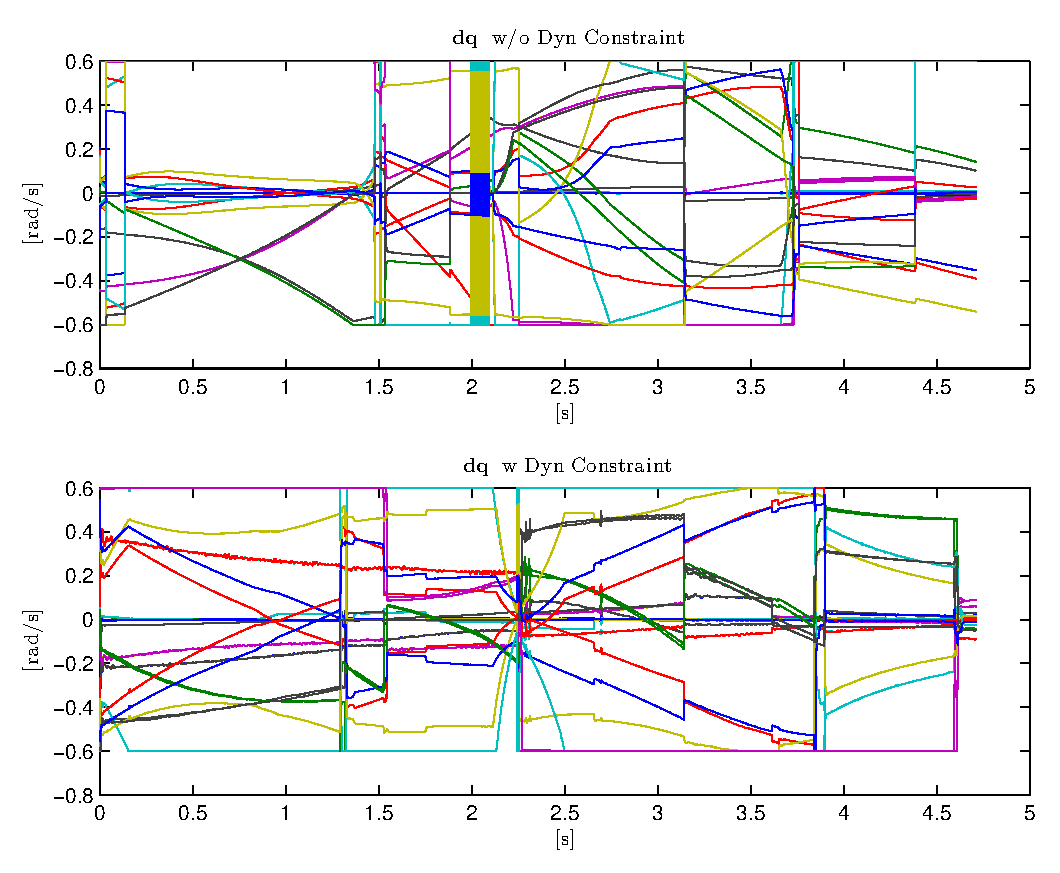
\includegraphics{images/dyn/dq_dyn.eps} \caption{Computed joint velocities}
%        \label{dq_dyn}
    %\end{subfigure}
%\end{sidewaysfigure}
%\newpage
%\begin{sidewaysfigure}
%    \centering
    %\begin{subfigure}[b]{0.8\textwidth}
%        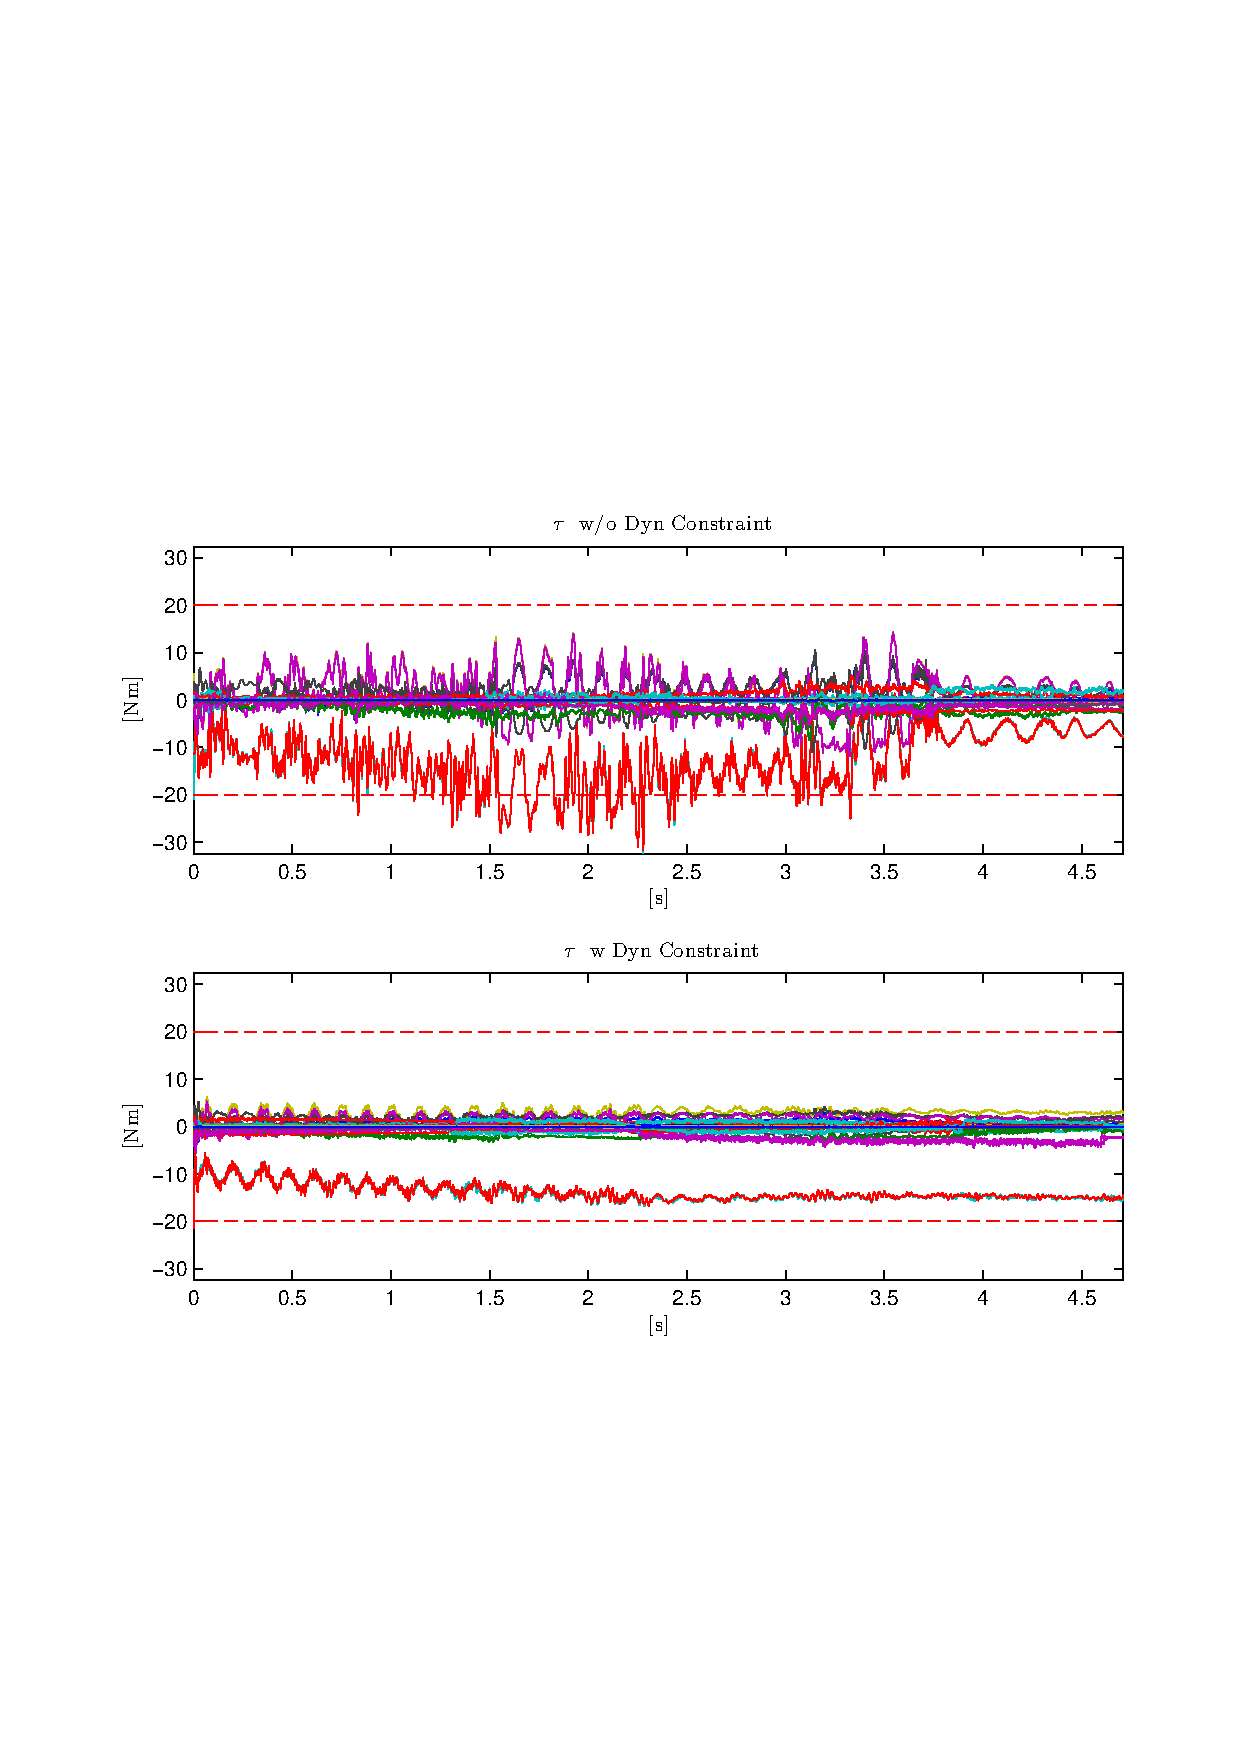
\includegraphics[width=\textwidth]{images/dyn/tau_dyn.png}
        %\caption{Dynamics of the Cartesian error}
        %\label{Cartesian_error}
    %\end{subfigure}
%    \caption{Computed joint torques}\label{tau_dyn}
%\end{sidewaysfigure}
%\clearpage

We will now show the application of the robot dynamics Constraint into a complex IK problem to perform a Cartesian task with the simulated model of our humanoid robot WALK-MAN (in Fig \ref{walkman_kinematics}). The task consists of moving the left arm forward and near the ground generating a squat motion of the whole body and high joint torques. We will show not only that the joint torques are bounded in the limits but also that the task makes the robot fall if performed without the robot dynamics constraint. 

Apart from the robot dynamics constraint, we consider joint limits, joint velocity limits (up to $0.9 \ \left[ \frac{rad}{sec} \right]$), the Center of Mass of the robot has to lie inside the support polygon and self collision avoidance. 
The self collision avoidance constraint makes use of capsules as bounding volumes to approximate the link geometries of the robot, in order to compute the minimum distance between colliding links.

\begin{figure}[htb] 
\centering 
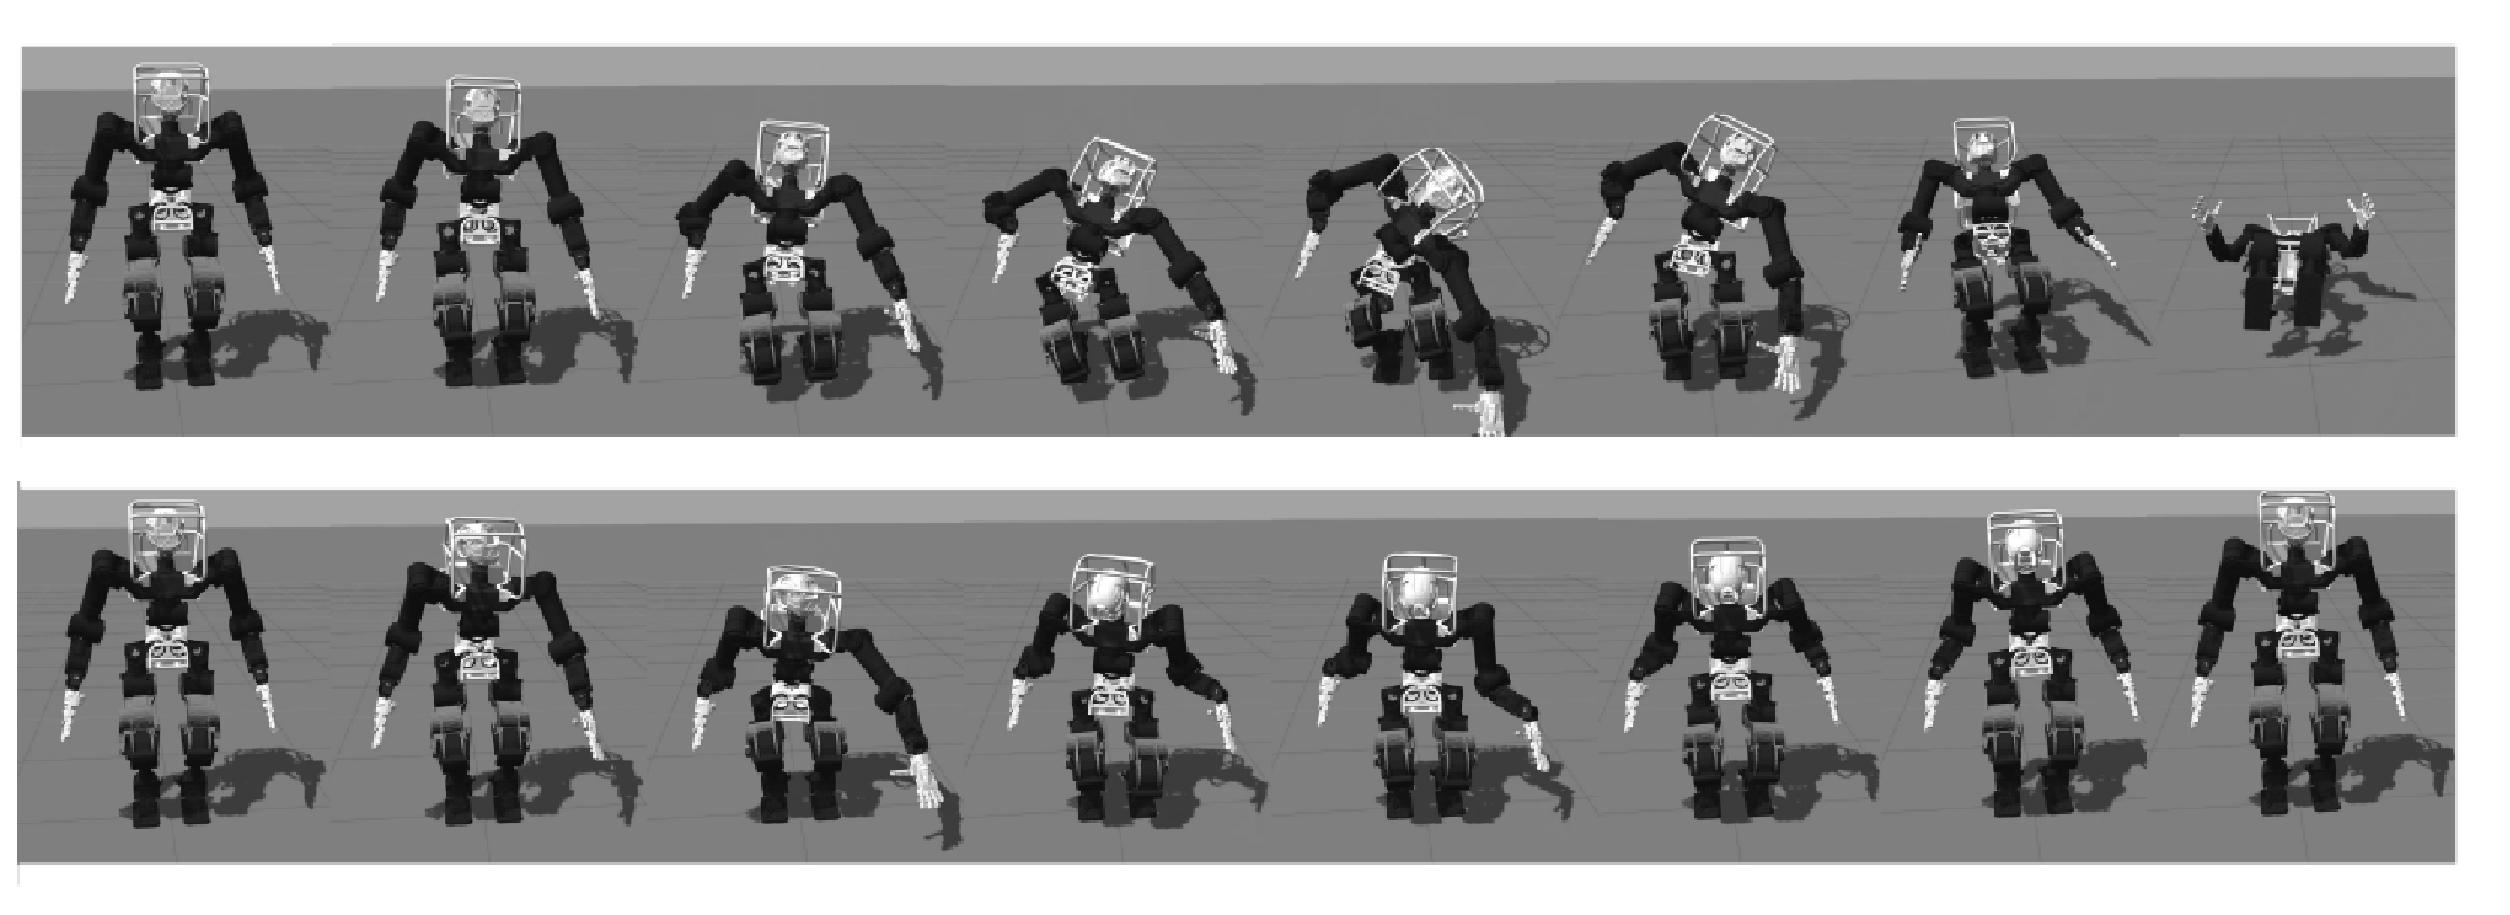
\includegraphics[width=\textwidth]{images/dynamic_constr.eps} 
\caption{In the upper sequence WALK-MAN falls due to a dynamically unfeasible motion while in the lower sequence the motion is dynamically feasible thanks to the dynamics constraint} 
\label{motion_dyn_constr}
\end{figure}

For the robot dynamics constraint we are using $\sigma = 0.2$ and we are filtering the sensed (simulated) wrenches at the force/torque sensors using a simple filter:
\begin{equation}
\mathbf{w}_\text{t} \mathrel{{+}{=}} \left( \mathbf{w}_\text{t} - \mathbf{w}_\text{t-1} \right) 0.6
\end{equation}
Furthermore we want to limit the amount of torque used in the torso to perform the task: in particular, for the three joints in the torso we set a maximum of $72 \left[ Nm\right]$ for the roll joint, $132 \left[ Nm\right]$ for the pitch joint and $72 \left[ Nm\right]$ for the yaw joint (around $40\%$ less than the maximum available peak torques in the real robot). 

The Cartesian task consists of a linear trajectory for the left hand, from the initial pose, $0.7 \left[ m \right]$ forward, $0.08 \left[ m \right]$ on the left, $0.5 \left[ m \right]$ down and it has to rotate around the $z$ axis of $\frac{\pi}{3} \left[ rad \right]$ and then back again. The trajectory has to be executed in 6 seconds. Desired joint trajectories are sent to the robot open-loop integrating the results obtained from the IK:
\begin{equation}
\q_\text{d} = \q + \dq \Delta T
\end{equation}

\begin{figure}[htb] 
\centering 
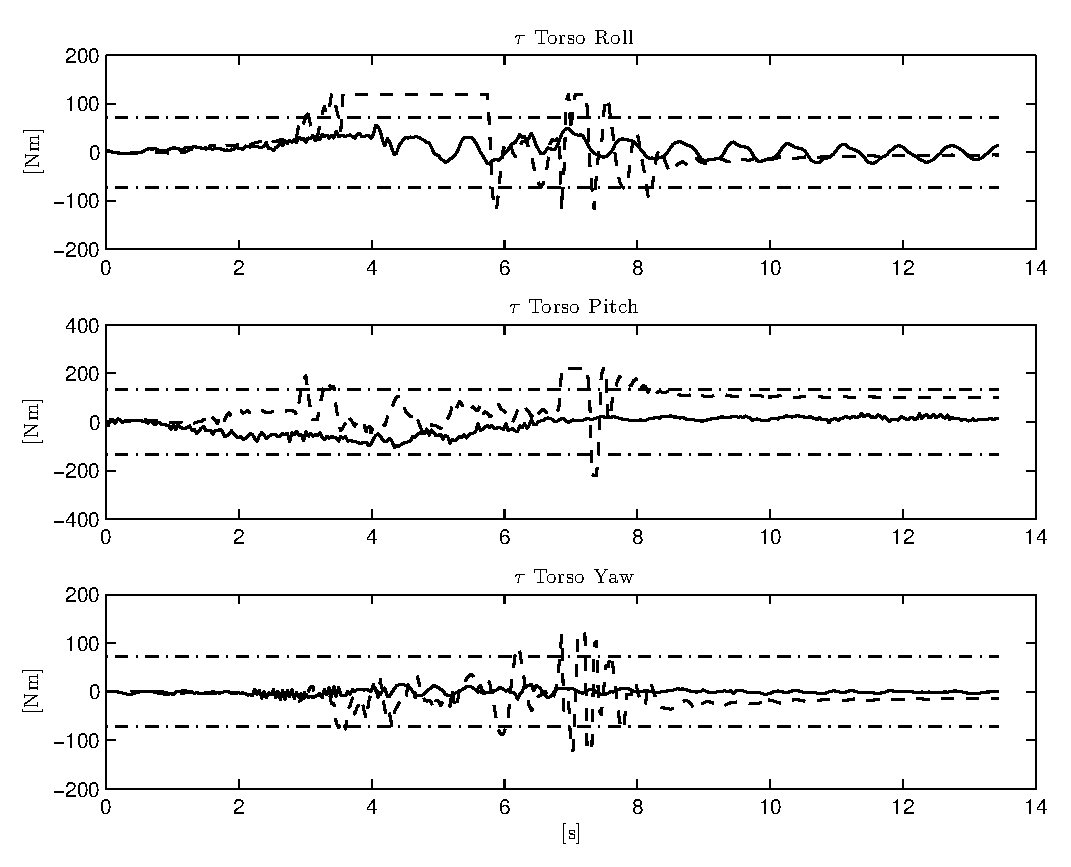
\includegraphics[width=\textwidth]{images/tau_torso.eps} 
\caption{Measured torques on the joints of the torso while performing the task without (dashed lines) and with (continuous lines) the robot dynamics constraint. The constant lines shows the limits on the torques} 
\label{tau_torso}
\end{figure}

In Fig. \ref{motion_dyn_constr} it can be observed the final motion performed by the robot when the robot dynamics constraint is not active (upper sequence) and when it is active (lower sequence). Without considering torque limits the robot falls in the second part of the squat motion. Fig. \ref{tau_torso} shows that the torques at the torso remains in the limits when using the robot dynamics constraint, while saturate when not using it.

\begin{figure}[htb] 
\centering 
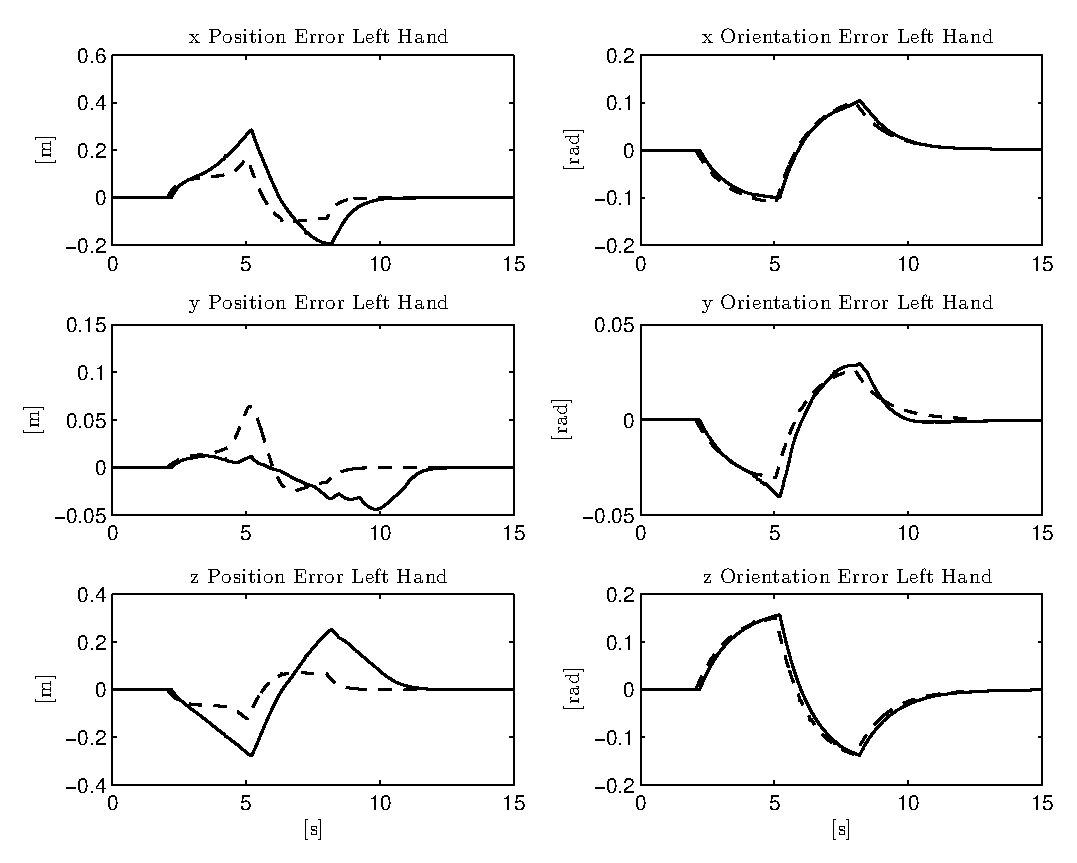
\includegraphics[width=\textwidth]{images/cartesian_error.eps} 
\caption{Cartesian error on the left hand while performing the task without (dashed lines) and with (continuous lines) the robot dynamics constraint} 
\label{cartesian_error}
\end{figure}

Cartesian errors are shown in Fig. \ref{cartesian_error}. Despite the Cartesian errors are small when not using the robot dynamics constraint, the robot falls with high joint torques trying to keep the Cartesian error small. With the constraint activated, the Cartesian errors are larger but the robot does not fall and the torques on the joints are inside the bounds. 

% REMOVED 05/02/16
% \paragraph{Interaction}
% In this example the robot has to reach the wall with the right arm and regulate the interaction wrench. The desired wrench at the contact is $\mathbf{w}_\text{d} = \left[25.0, \ 0.0, \ 0.0, \ \mid \ 0.0, \ 0.0, \ 0.0 \right] \quad \left[N \ \mid \ Nm \right]$. The compliance matrix $C$ is:
% \begin{equation}
% C = \begin{bmatrix}
% 10^{-5} & 0 & 0 & 0 & 0 & 0\\ 
% 0 & 10^{-5} & 0 & 0 & 0 & 0\\ 
% 0 & 0 & 10^{-5} & 0 & 0 & 0\\ 
% 0 & 0 & 0 & 10^{-4} & 0 & 0\\ 
% 0 & 0 & 0 & 0 & 10^{-4} & 0\\ 
% 0 & 0 & 0 & 0 & 0 & 10^{-4}
% \end{bmatrix}
% \end{equation}
% \begin{figure*}[!h]
% \vspace{2 mm}
% \centering
% 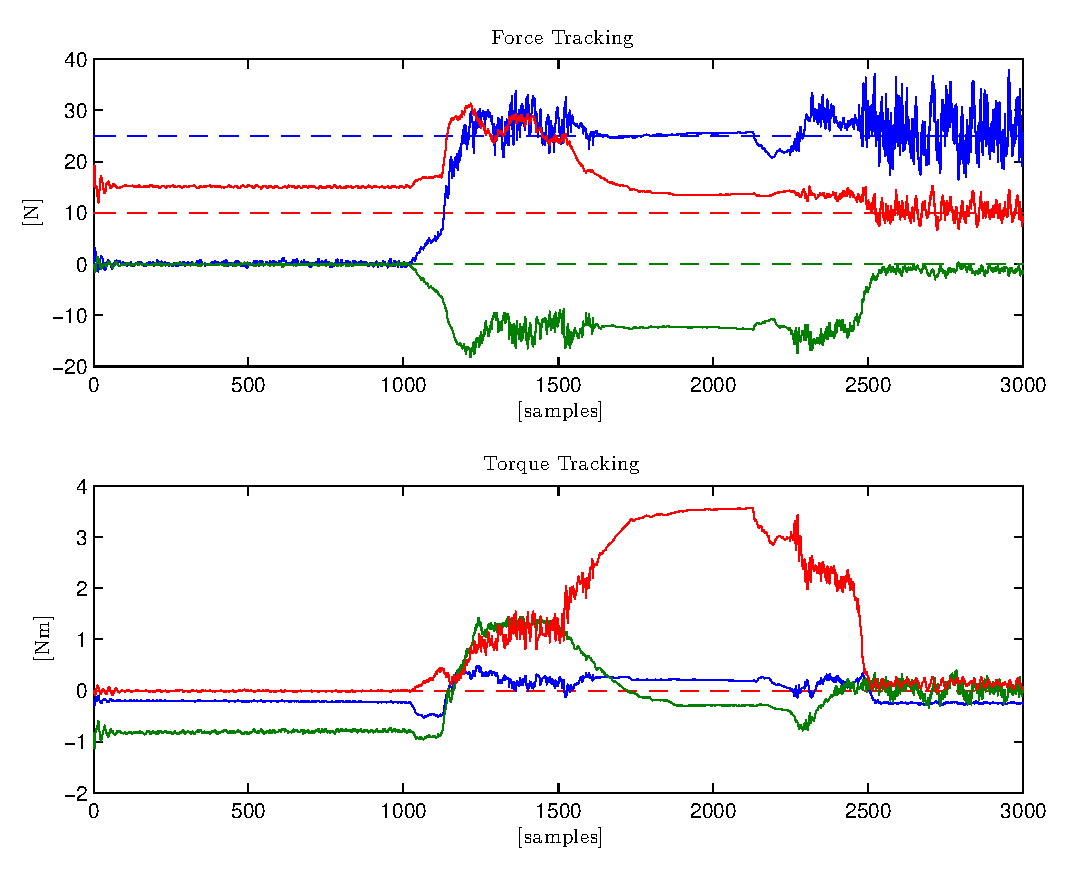
\includegraphics[width=0.7\textwidth]{images/interaction/wrench_tracking.eps}
% \caption{Wrench tracking with the interaction task}
% \label{wrench_tracking}
% \end{figure*}
% 
% The IK problem is composed by:
% \begin{equation}
% \begin{pmatrix}
% T_{\substack{\text{Interaction}\\\text{Right Arm}}}\setminus\\
% \\
% T_{\substack{\text{Joint}\\\text{Posture}}}
% \end{pmatrix}
% << \left(B_{\substack{\text{Joint}\\\text{Limits}}} + B_{\substack{\text{Joint Velocity}\\\text{Limits}}}\right)
% \end{equation}
% Figure \ref{wrench_tracking} shows the tracking of the desired wrench while Figure \ref{interaction_COMAN} shows the motion performed by COMAN in simulation.
% \begin{figure*}[!h]
% \vspace{2 mm}
% \centering
% 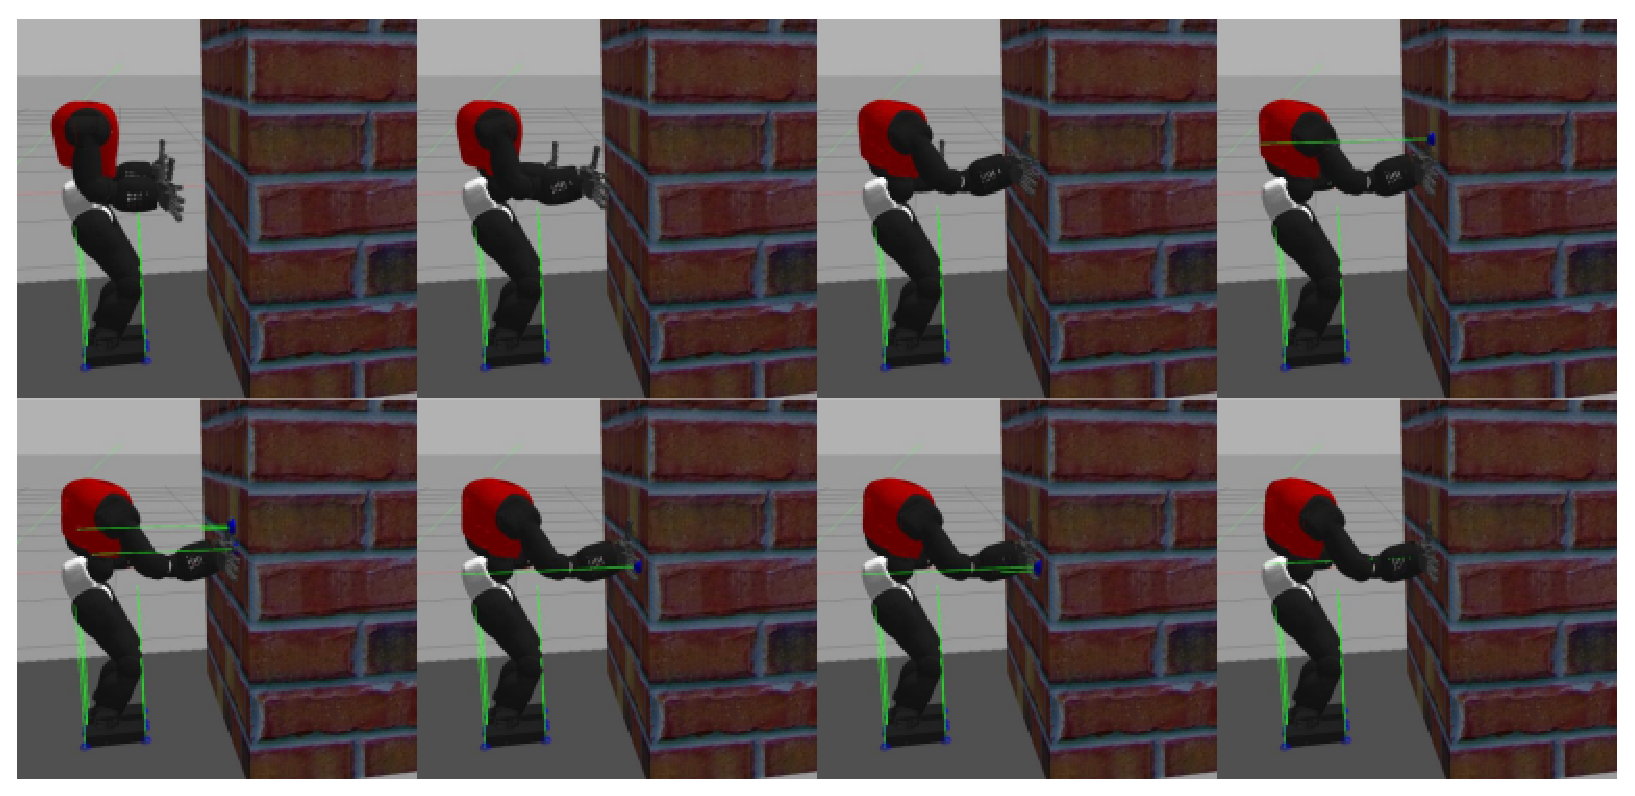
\includegraphics[width=0.7\textwidth]{images/interaction/interaction.eps}
% \caption{COMAN performing the interaction task with the right arm, blue dots shows the contact points}
% \label{interaction_COMAN}
% \end{figure*}

\paragraph{Resources Allocation: Velocity Allocation}
\label{velocity_allocation}
When a high priority task saturates a given constraint, and in particular joint resources (i.e., joint velocity limits or joint torque limits) lower priority tasks will not have control authority to keep task error low. This situation is similar to what in real-time computing systems is called \emph{starvation}. In these cases, a small compromise on high priority task performance will provide a big increment in the ability of the lower priority tasks to perform, even when the robot has a high degree of redundancy. Such a compromise is non-linear in nature, since it is due to saturation, and will imply that hard priorities between tasks will be enforced, \emph{unless} the high priority task requires too many resources from the system. A possible solution in order to implement this scheme, is \emph{resource allocation}. The constraints for each task will be \emph{scaled}, where constraints for higher priority tasks will be more stringent to constraints of lower priority tasks. Such scaling $\sigma_i$, with
\begin{equation}
0 < \sigma_i \leq 1, \sigma_i \leq \sigma_{i+1}
\label{eq:scaling_relation}
\end{equation}
where $i$ is the task priority (from $1$ to $n$), will be applied to the resource constraint on each task, and the maximum amount of resources \emph{exclusively} allocated to a certain task will be 
\begin{equation}
\rho = \sigma_i-\sigma_{i-1}
\end{equation}
where $\sigma_0 = 0$. A demonstration of such scheme is illustrated in Figure \ref{fig:velocity_allocation} for the following IK problem 
\begin{equation}
\begin{pmatrix}
\left(T_{\substack{\text{Right}\\\text{Foot}}} + T_{\substack{\text{Left}\\\text{Foot}}}\right)\setminus\\
\\
\left(T_{\substack{\text{Right}\\\text{Wrist}}} + T_{\substack{\text{Left}\\\text{Wrist}}}\right)
\end{pmatrix}
<< B_{\substack{\text{Joint Velocity}\\\text{Limits}}}
\end{equation}
The Velocity Allocation (VA) scheme in implemented in \textbf{OpenSoT} via the \texttt{VelocityAllocation} utility, which gets as input the minimum joint velocity constraint and maximum velocity constraint for a certain stack, and will apply the minimum value to the highest priority task, the maximum value to the higher priority task, and will apply a value equal to 
\begin{equation}
\text{res}_\text{min} + i \times \frac{\text{res}_\text{max} - \text{res}_\text{min}}{n-1}
\end{equation} for all the others, so that 
\begin{equation}
\rho_i=\frac{\text{res}_\text{max} - \text{res}_\text{min}}{\text{res}_\text{max} \times n-1}
\end{equation}. The VA can then be modified manually on each individual task, as long as the scaling relation \ref{eq:scaling_relation} is satisfied.

%The velocity allocation is specified in the code by usage of the \texttt{VelocityAllocation} utility, which is called as \texttt{VelocityAllocation(stack,dT,min\_vel,max\_vel,\emph{last\_vel=max\_vel})}

\begin{figure*}[!h]
\vspace{2 mm}
\centering
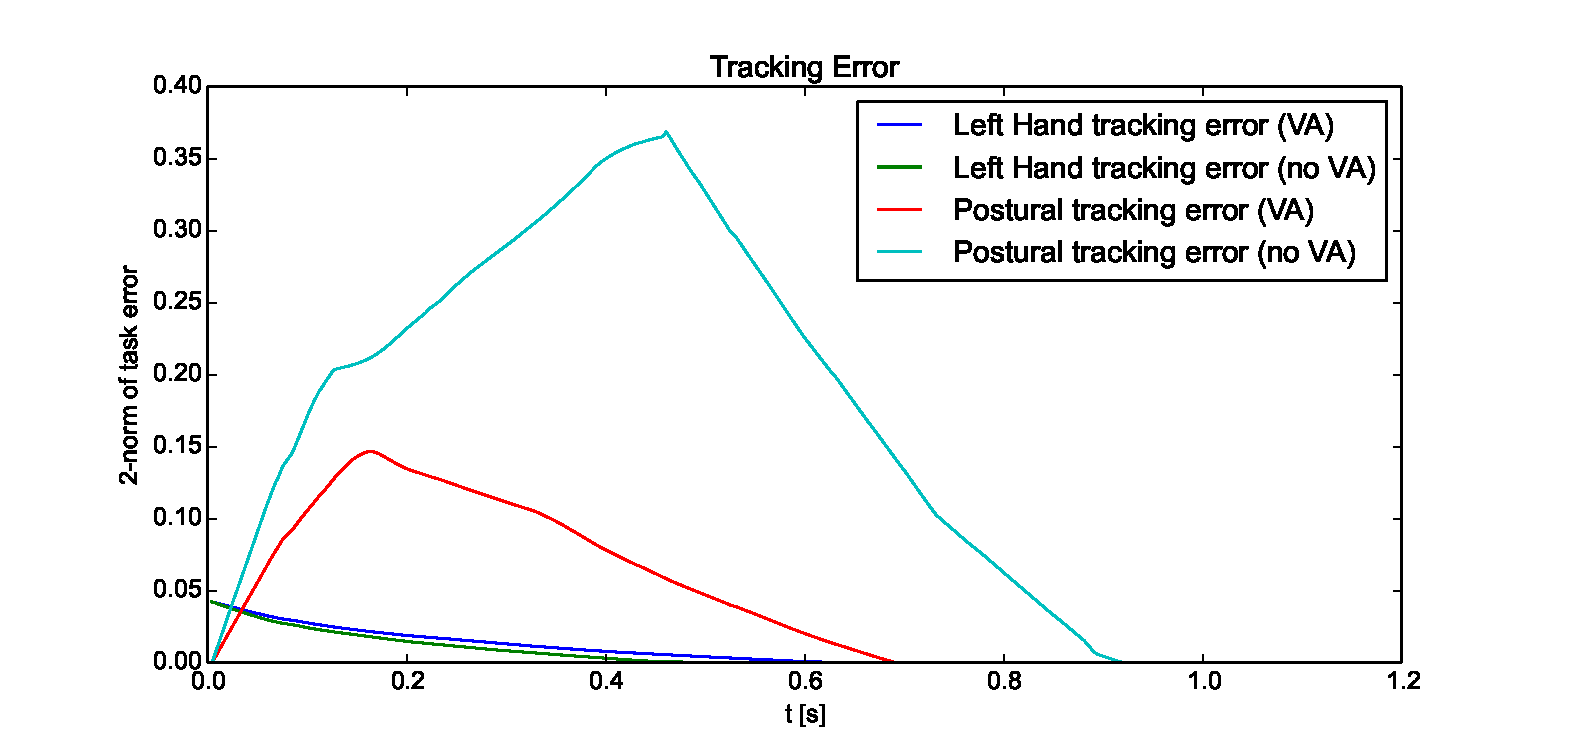
\includegraphics[width=0.7\textwidth]{images/sim_data/postural_vel_alloc}
\caption{When VA is active, all tasks in the stack have $0.15$, $0.225$, $0.3$ rad/s limits, otherwise $0.3$ rad/s for each task}
\label{fig:velocity_allocation}
\end{figure*}

\paragraph{Self Collision Avoidance} 
During tele-operation tasks, a mistake in providing task references, or the combination of safe task trajectories with null-space tasks, can cause self-collisions. In particular, while the former case can be filtered by means of a check on the provided references, the latter is inherent in the idea of trajectory-less tasks (such as minimum effort, manipulation maximization, joint acceleration minimization), so that providing these tasks with self-collision awareness is necessary. In Figure \ref{fig:sca} a tele-operation task is executed with a self collision avoidance (SCA) constraint active on all the levels of the stack.
The IK problem for the task is a whole-body task composed of
\begin{equation}
\begin{pmatrix}
T_{\substack{\text{Right}\\\text{Foot}}}\setminus\\
\\
T_{\text{CoM}_\text{XY}}\setminus\\ 
\\
\left(T_{\substack{\text{Right}\\\text{Wrist}}} + T_{\substack{\text{Left}\\\text{Wrist}}}\right)\setminus\\ 
\\
T_{\substack{\text{Joint}\\\text{Posture}}}
\end{pmatrix}
<< \left(B_{\substack{\text{Joint}\\\text{Limits}}} + B_{\substack{\text{Joint Velocity}\\\text{Limits}}} + C_{SCA}\right)
\end{equation}
The constraint activates on a certain pair of links when the distance between these two links is lower than a certain threshold. The maximum relative velocity between the two links in the direction of the minimum-distance segment between the two is then limited so to avoid interpenetration.

\begin{figure*}[!h]
\vspace{2 mm}
\centering
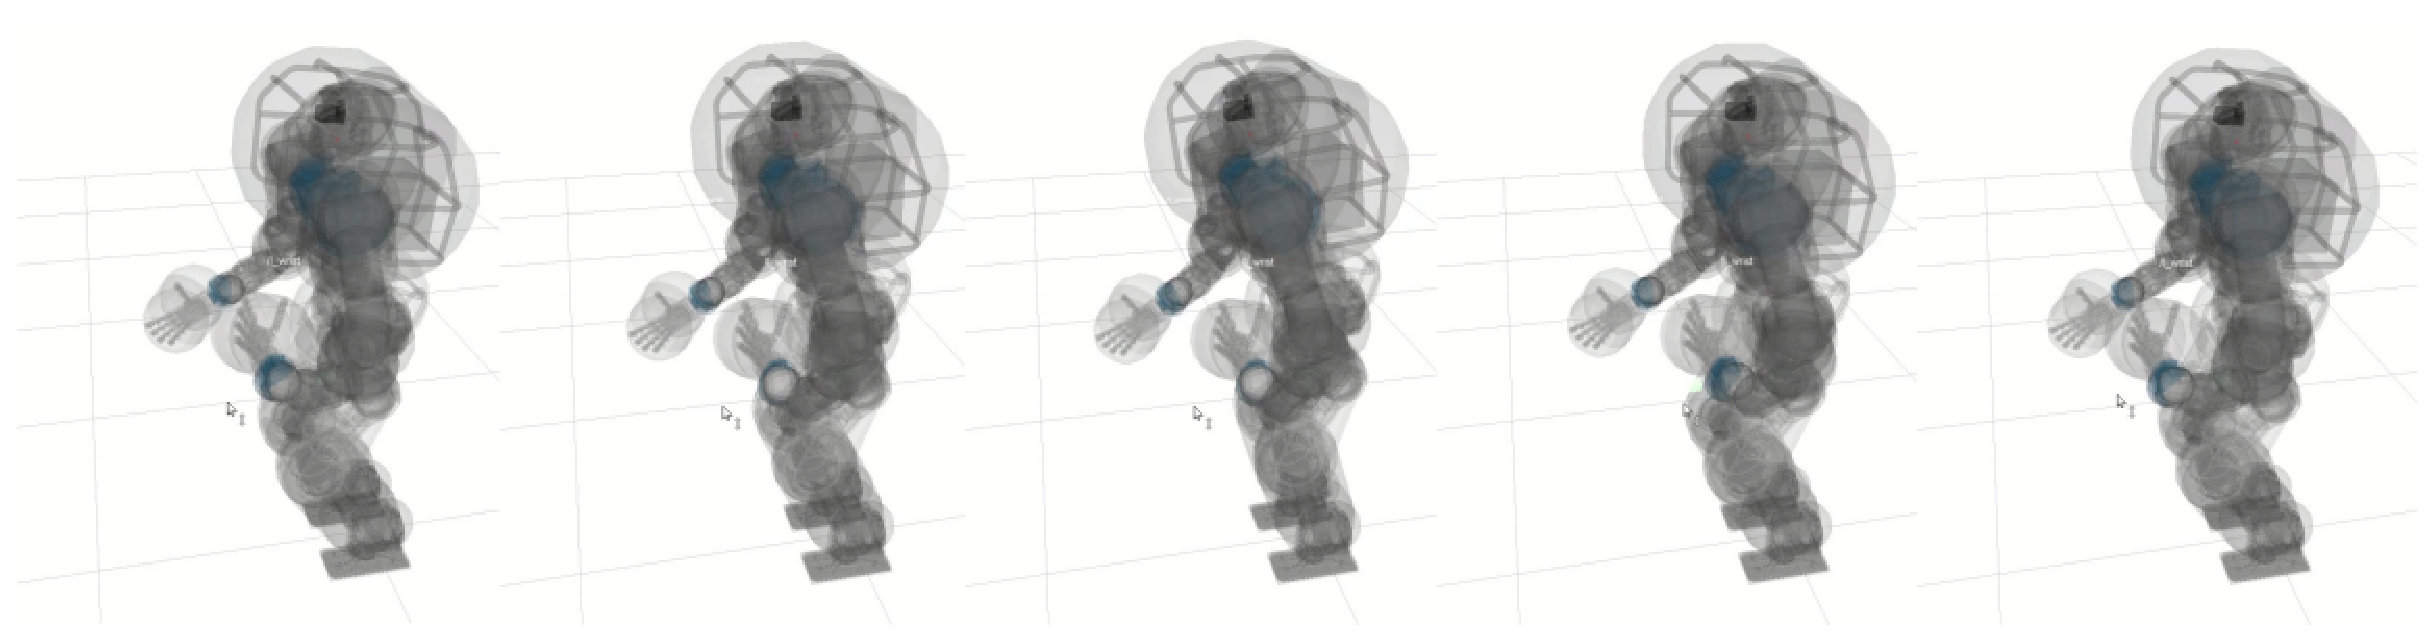
\includegraphics[width=\textwidth]{images/sca/sca}
\caption{Self Collision Avoidance (SCA) constraint on the Walk-Man robot.  When the left wrist reference is too close to the body so as to cause a possible collision, the robot reconfigures itself by moving the waist back}
\label{fig:sca}
\end{figure*}

\subsubsection{Solver}
In this section we show some results regarding the IK solver distributed with the \textbf{OpenSoT} library. In the first one we compare the results between the sparse and the dense implementation of the IK solver. In the second one we compare the quality of the generated joint trajectory changing the $\lambda$ parameter. 

\subsubsection{Sparse implementation}
Most of the time, the cost function \ref{cost_function}
will result in a sparse matrix (in some particular cases this is not true, for instance when controlling the Center of Mass of the robot) with a dimension $m \times n$ where $m$ is the dimension of the task and $n$ is the number of the joints.  
It is possible to use the sparsity of the matrices in order to speed up the computation: in particular, \emph{qpOASES} permits to define QP Problems in which Hessian matrices are sparse. However we have tested the performances of the sparse implementation against the dense implementation (in the dense implementation we do not use special data structure for sparse matrices) and we found that, for a medium size IK Problem (29 variables, up to 63 constraints), the real advantage is in the \emph{initialization} phase where the sparse solver is around twice faster than the dense solver. The IK Problem consists in 3 stacks: 
\begin{equation}
\begin{pmatrix}
T_{\substack{\text{Right}\\\text{Foot}}}\setminus\\
\\
\left(T_{\substack{\text{Right}\\\text{Wrist}}} + T_{\substack{\text{Left}\\\text{Wrist}}} + T_\text{Waist} + T_\text{Torso}\right)\setminus\\ 
\\
\left(T_{\substack{\text{Joint}\\\text{Posture}}} + T_{\substack{\text{Minimum}\\\text{Acceleration}}}\right)
\end{pmatrix}
<< \left(B_{\substack{\text{Joint}\\\text{Limits}}} + B_{\substack{\text{Joint Velocity}\\\text{Limits}}} + C_{\substack{\text{CoM}\\\text{ConvexHull}}} 
+ C_{\substack{\text{CoM Velocity}\\\text{Limits}}}\right)
\end{equation}

Results (in seconds) are reported in Table \ref{sparse_vs_dense}.
\begin{table}[!hb]
\centering
\caption{Sparse Vs Dense}
\label{sparse_vs_dense}
\begin{tabular}{lccll}
\cline{2-3}
\multicolumn{1}{l|}{}  & \multicolumn{1}{c|}{Initialization} & \multicolumn{1}{c|}{Solve} &  &  \\ \cline{1-3}
\multicolumn{1}{|l|}{Sparse} & \multicolumn{1}{c|}{0.00143099} & \multicolumn{1}{c|}{0.000490187} &  &  \\ \cline{1-3}
\multicolumn{1}{|l|}{Dense} & \multicolumn{1}{c|}{0.00297189} & \multicolumn{1}{c|}{0.000475262} &  &  \\ \cline{1-3}
                       & \multicolumn{1}{l}{}  & \multicolumn{1}{l}{}  &  & 
\end{tabular}
\end{table}
We see how the run takes around 0.5 ms for both the solvers while the initialization takes around 1.5 ms for the Sparse solver and around 3 ms for the Dense solver. Figure \ref{solver_time} shows the trends of the \emph{Sparse} solver Vs the \emph{Dense} solver, the first one has a variance of 9.4777e-10, the latter of 2.3904e-09 (the \emph{Sparse} solver is more constant).
\begin{figure}[htb!]
\vspace{2 mm}
\centering 
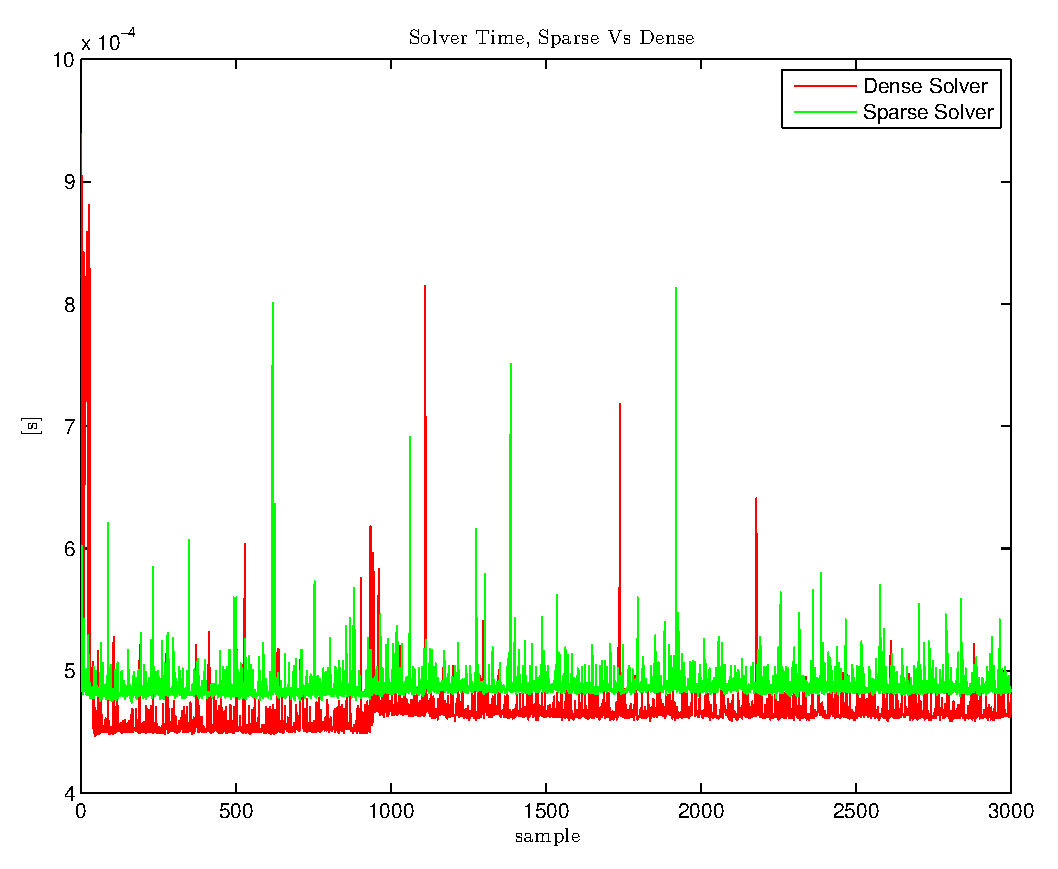
\includegraphics[width=0.6\linewidth]{images/wholebody/solverTime3.eps} 
\caption{Time needed to solve a stack of tasks, Sparse vs. Dense implementation} 
\label{solver_time}
\end{figure}
The solver can be clearly used for 1 ms real-time control. %Considering also the comparison in \cite{Beeson15}, between another IK solver used in the DRC Finals, our IK solver perform better in terms of time and capabilities.  

\subsubsection{Task execution and Regularisation}
Here we show the effect of changing the regularisation term as well as  the tracking performances in our IK solver. We consider a complex, whole-body, manipulation task composed by:
\begin{equation}
\begin{pmatrix}
\left(T_{\substack{\text{Right}\\\text{Foot}}} + T_{\substack{\text{Joint}\\\text{Posture Torso}}}\right)\setminus\\
\\
\left(T_{\substack{\text{Right}\\\text{Wrist}}} + T_{\substack{\text{Left}\\\text{Wrist}}} + T_\text{Gaze} + T_\text{Waist} + T_\text{CoM}\right)\setminus\\ 
\\
\left(T_{\substack{\text{Joint}\\\text{Posture}}} + T_{\substack{\text{Min}\\\text{Acceleration}}}\right)
\end{pmatrix}
<< \left(B_{\substack{\text{Joint}\\\text{Limits}}} + B_{\substack{\text{Joint Velocity}\\\text{Limits}}} + C_{\substack{\text{CoM}\\\text{ConvexHull}}}\right)
\end{equation}
The \emph{Gaze} task is built on top of the Cartesian task using the method presented in \cite{milighetti:2011}.
Some references, in terms of Cartesian trajectories (linear and circular) and constant poses for the end-effectors, are sent by the user. Computed joint trajectories are sent to the simulated robot integrating the initial value at each iteration (open-loop):
\begin{equation}
    \mathbf{q}_\text{k} = \mathbf{q}_\text{k-1} + \mathbf{\Delta q}
    \label{open_loop}
\end{equation}
where $\mathbf{\Delta q}$ is computed by our IK solver. Two experiments were performed changing the value of the $\lambda$ in the regularisation term: the first one with $\lambda = 2.221\cdot10^{-3}$, the second with $\lambda = 2.221\cdot10^{-13}$. The results in Figures \ref{Cartesian_error} and \ref{joint_trj_vel} clearly shows how this affects the resulting smoothness of the joints trajectories, as well as joint velocities and Cartesian error. In particular we see that high values of $\lambda$ are associated with more smoothness of joint trajectories and velocities against higher values of Cartesian error during task execution. It is also clear how with high values of $\lambda$, joints velocities tend to saturate less. The average time that a solve takes, for the first run, is $8.4062 \cdot 10^{-4} \ [s]$, while for the second is $8.0448 \cdot 10^{-4} \ [s]$, the controller runs at 100Hz. The IK Problem has a total of 31 variables and up to 61 constraints.
\begin{figure*}
\vspace{2 mm}
\centering
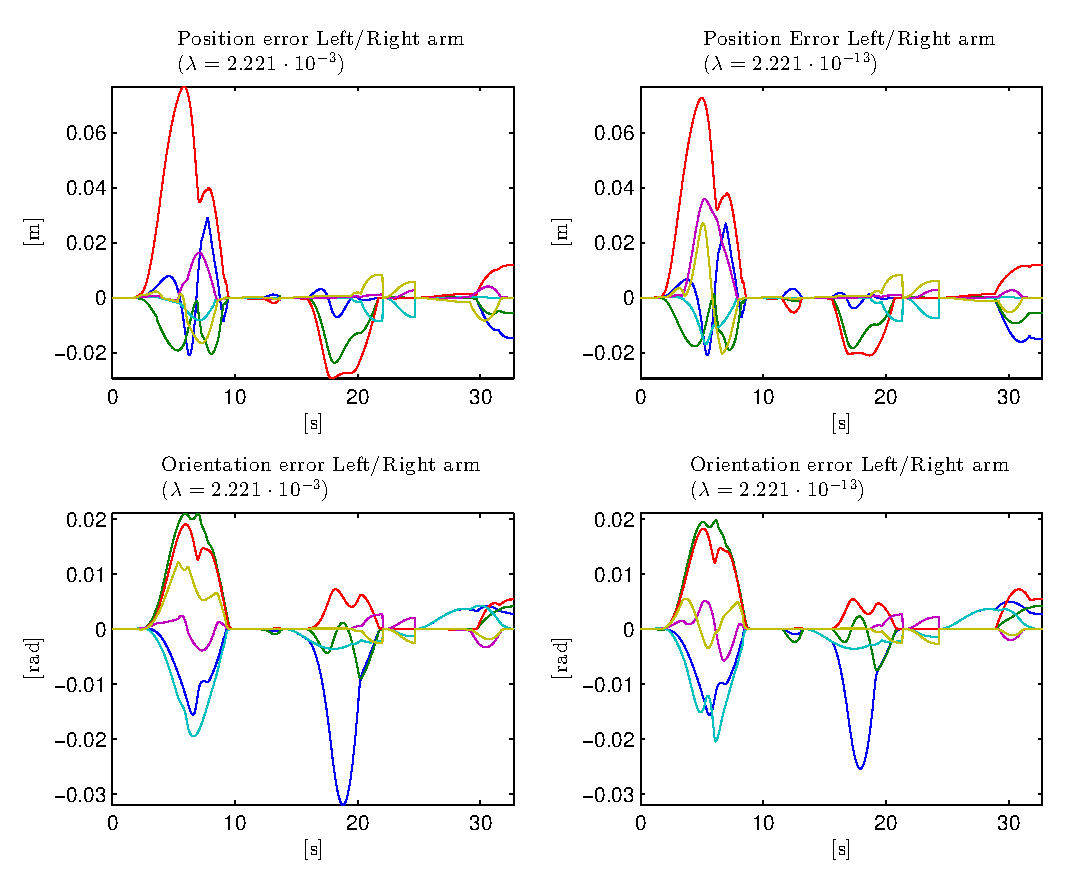
\includegraphics[width=0.85\textwidth]{images/wholebody/Cartesian_error.eps}
\caption{Cartesian error for two different values of $\lambda$ in task execution}
\label{Cartesian_error}
\end{figure*}

\begin{figure*}
    \vspace{2 mm}
    \centering
    \begin{subfigure}[b]{\textwidth}
        \centering
        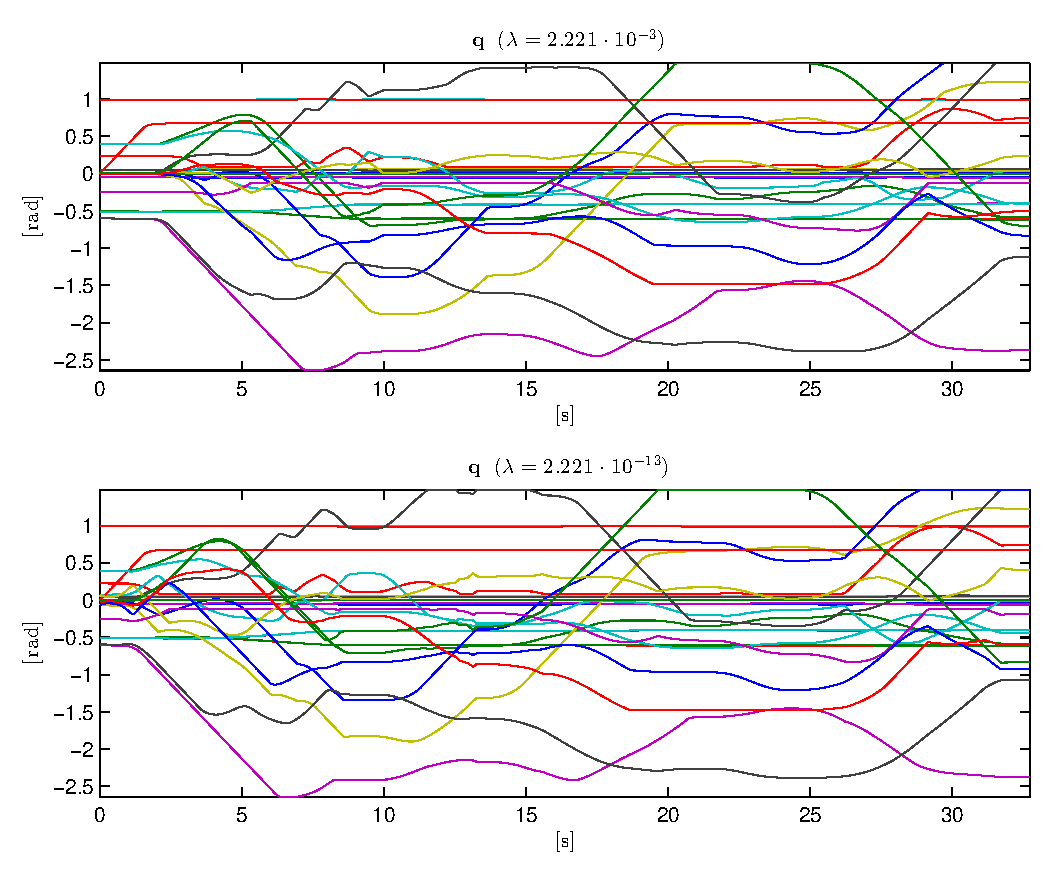
\includegraphics[width=0.8\textwidth]{images/valve_lambda_exp/q.eps} %\caption{Computed joint trajectories for two different values of $\lambda$ in task execution}
        %\label{joint_trj}
    \end{subfigure}

    \begin{subfigure}[b]{\textwidth}
        \centering
        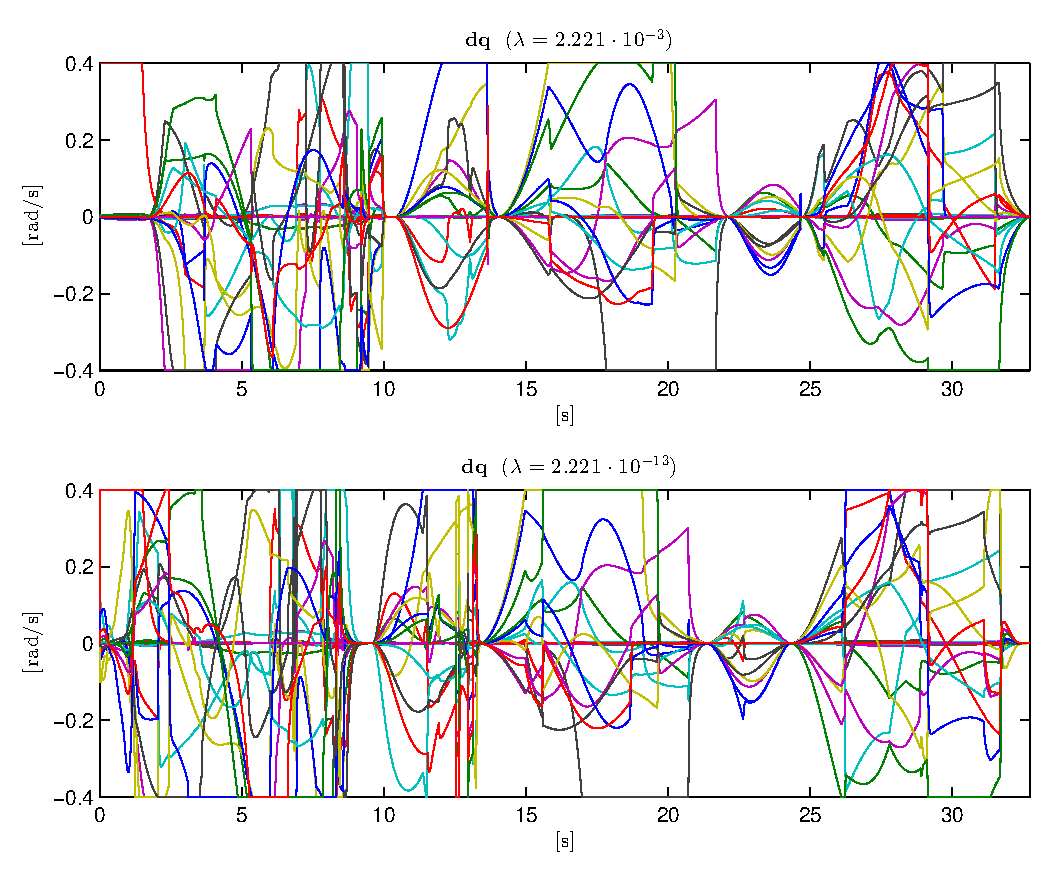
\includegraphics[width=0.8\textwidth]{images/valve_lambda_exp/dq.eps} %\caption{Dynamics of the Cartesian error}
        %\label{Cartesian_error}
    \end{subfigure}
    \caption{Computed joint trajectories and joint velocities for two different values of $\lambda$ in task execution. Notice how bigger $\lambda$ values correspond to smoother trajectories (e.g. at secs $10-12$ and $23-24$) }
    \label{joint_trj_vel}
\end{figure*}

%\begin{sidewaysfigure}
%    \centering
    %\begin{subfigure}[b]{0.8\textwidth}
%        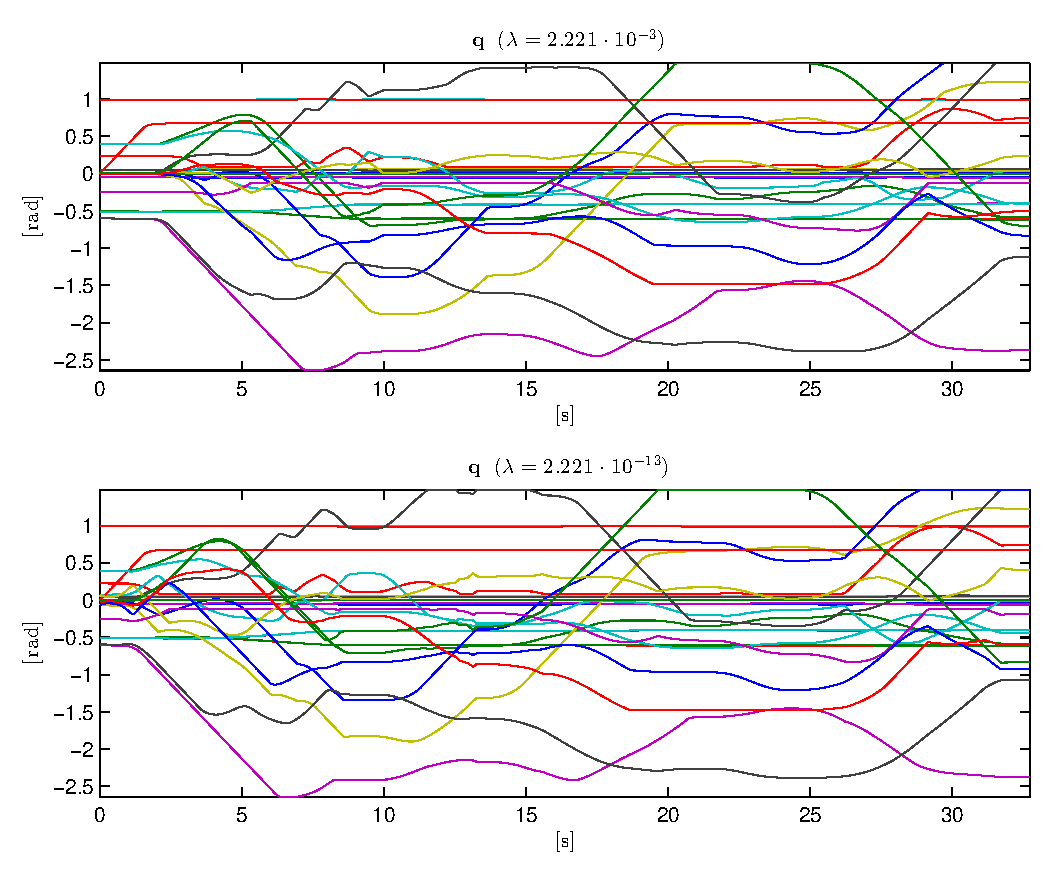
\includegraphics{images/valve_lambda_exp/q.eps} \caption{Computed joint trajectories for two different values of $\lambda$ in task execution}
%        \label{joint_trj}
    %\end{subfigure}
%\end{sidewaysfigure}

%\begin{sidewaysfigure}
%    \centering
    %\begin{subfigure}[b]{0.8\textwidth}
%        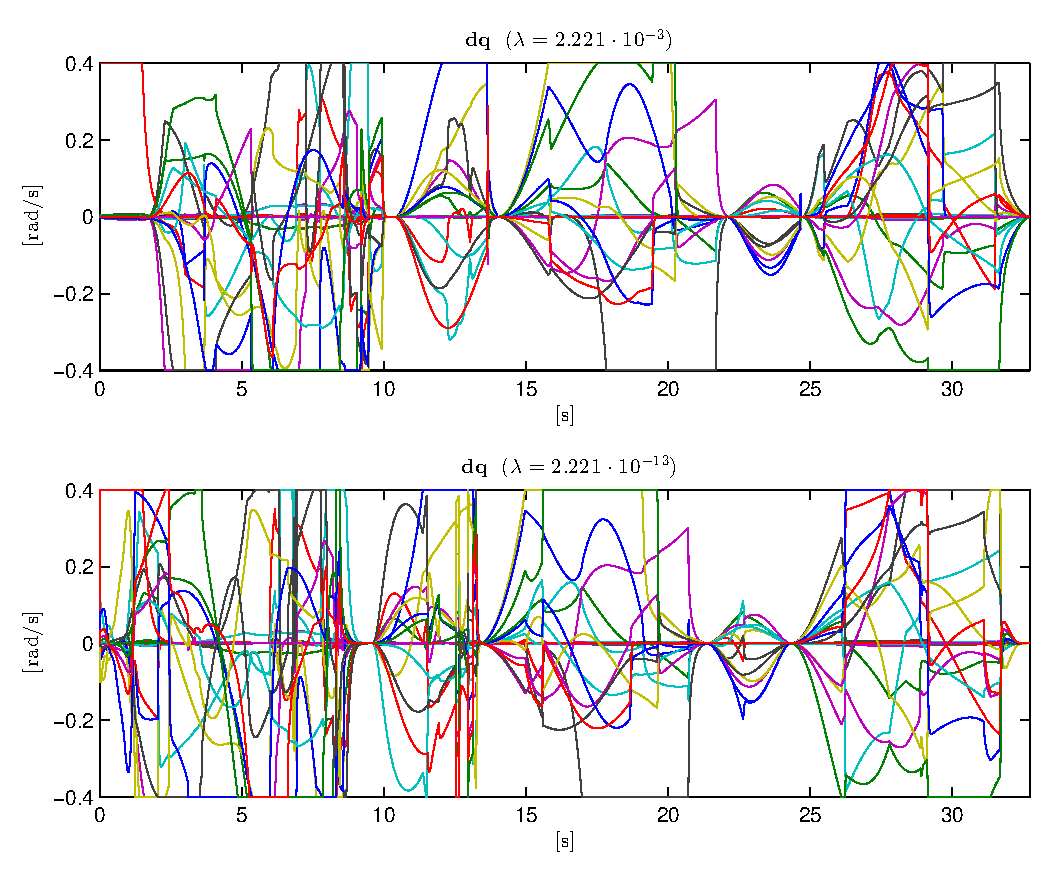
\includegraphics{images/valve_lambda_exp/dq.eps}
        %\caption{Dynamics of the Cartesian error}
        %\label{Cartesian_error}
    %\end{subfigure}
%    \caption{Computed joint velocities for two different values of $\lambda$ in task execution}\label{joint_vel}
%\end{sidewaysfigure}

\subsection{The Darpa Robotics Challenge}
\begin{figure*}
\vspace{2 mm}
\centering 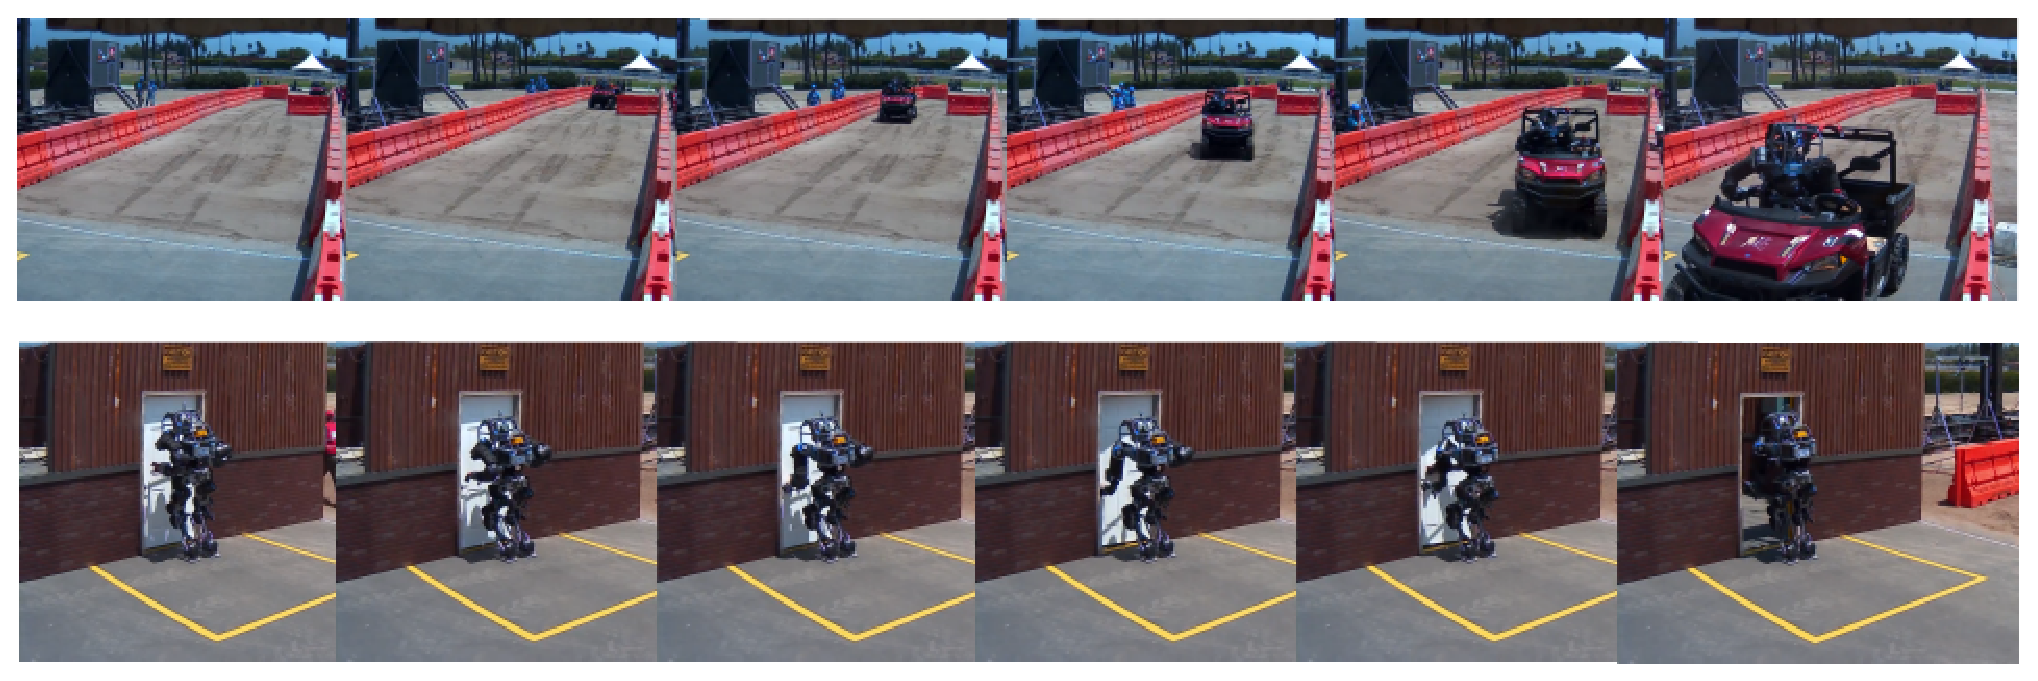
\includegraphics[width=\textwidth]{images/wholebody/walkman_drc.eps} 
\caption{WALK-MAN during DRC Finals completed two tasks: \emph{driving} and \emph{door opening}} 
\label{walkman_drc}
\end{figure*}
In the DRC Finals the presented library was used to implement all the manipulation tasks (\emph{driving}, \emph{door opening}, \emph{wall cutting} and \emph{valve turning}) while keeping balance as well as considering joint limits and joint velocity limits. Two of them were performed during the finals: \emph{driving} and \emph{door opening}. 
For the \emph{drive} task the IK problem used was:
\begin{equation}
\begin{pmatrix}
T_{\substack{\text{Left}\\\text{Foot}}}\setminus\\
\\
T_{\substack{\text{Left}\\\text{Wrist}}}
\end{pmatrix}
<< \left(B_{\substack{\text{Joint}\\\text{Limits}}} + B_{\substack{\text{Joint Velocity}\\\text{Limits}}}\right)
\end{equation}

For the \emph{door} task the IK problem used was:
\begin{equation}
\begin{pmatrix}
T_{\substack{\text{Right}\\\text{Foot}}} << C_{\substack{\text{CoM}\\\text{Velocity}}}\setminus\\ 
\\
\left(T_\text{Waist} + T_\text{CoM}\right)  << C_{\substack{\text{CoM}\\\text{Velocity}}}\setminus\\ 
\\
\left(T_{\substack{\text{Left}\\\text{Wrist}}} + T_{\substack{\text{Right}\\\text{Wrist}}}\right)\setminus\\
\\
T_{\substack{\text{Joint}\\\text{Postural}}}
\end{pmatrix}
<< \left(B_{\substack{\text{Joint}\\\text{Limits}}} + B_{\substack{\text{Joint Velocity}\\\text{Limits}}}\right)
\end{equation}
and velocity allocation strategy.

The IK solver was running in the on-board computer of the WALK-MAN robot and the trajectories were sent to the joint servos using (\ref{open_loop}). Joints were controlled using position control.  WALK-MAN always accomplished the \emph{driving} and \emph{door opening} tasks (Figure \ref{walkman_drc}) in both the runs of the DRC Finals\footnote{http://www.theroboticschallenge.org/finalist/walk-man}.

\subsubsection{Conclusions}
\label{sec:conclusions}
This work introduced a novel whole-body control library called \textbf{OpenSoT}. Such framework allows to control a robot by solving a hierarchy of tasks with linear constraints. 
%The framework provides a library of already implemented tasks, constraints, bounds and solvers as well as an easy way to implement new ones by providing common interfaces.
Theoretical details about tasks, constraints and the IK solver available in the framework has been shown. In particular, the proposed IK solver satisfy the requirements in terms of robustness: singularity robustness, constraints/bounds specification and it permits to set priorities between tasks. The IK solver is composed by a \emph{front-end}, that prepares the IK Problem for the QP solver which constitutes the \emph{back-end}. As QP solver, a state-of-art library called qpOASES has been used.
%The \textbf{OpenSoT} framework contains also a set of tools to use the library with different robotic frameworks and high level programming languages, as well as facilitate the evaluation of the resulting computed trajectories.
%The performances of the library have been evaluated with a set of experiments and tests in multiple robotic platforms. \textbf{OpenSoT} was used by the WALK-MAN Team during the DRC Finals to perform all the manipulation tasks showing the possibility to use the framework in a real scenario.
The set of tasks and constraints considered permits to perform high-level tasks without damaging the robot. Experiments presented in this section demonstrated the usefulness and the capabilities of the library.

We also presented a new constraint for the QP based IK, for fixed/floating base robots, that takes in consideration the robot dynamics to filter dynamically unfeasible motions. We presented the theoretical formulation and we showed results in simulation using our humanoid robot WALK-MAN considering a whole body task involving also other constraints such as joint limits, joint velocity limits, the Center of Mass of the robot has to lie inside the support polygon and self collision avoidance. We show that the robot dynamics constraint can make the task dynamically feasible and it is able to keep the torques at the torso on the given boundary limits. We think this is fundamental when working on real hardware as well as joint limits and joint velocity limits. This constraint is fundamental when Cartesian trajectories references are \emph{aggressive}, for instance when considering motion capture data. 

Future work will entail adding more tasks and constraints at the velocity level, add acceleration and torque tasks and constraints and explore different solvers.

This work is the second and last part in a series of papers introducing a novel whole-body control library called \textbf{OpenSoT}. Such framework allows to control a robot by solving a hierarchy of tasks with linear constraints. 
The framework provides a library of already implemented tasks, constraints, bounds and solvers as well as an easy way to implement new ones by providing common interfaces.

We addressed the theoretical foundations of the framework, and presented a large set of experiments with the intent of demonstrating the robustness of the library, its successful use in real-case scenarios, and the richness of features.

We showed how the \textbf{OpenSoT} framework contains a set of tools allowing the use of the library in conjunction with different robotic frameworks and high level programming languages, as well as facilitate the behcmarking of the resulting computed trajectories.

The performances of the library have been evaluated with a set of experiments and tests in multiple robotic platforms. \textbf{OpenSoT} was used by the WALK-MAN Team during the DRC Finals to perform all the manipulation tasks showing the possibility to use the framework in a real scenario.

Even if \textbf{OpenSoT} is a young project, it showed its ease of use by a large groups of first-time users with varying backgrounds and education levels that programmed tasks for the DRC Finals in a very short amount of time. Its flexible API allowed researchers\cite{Fang2015-cr} to easily extend it and successfully implement research code on top of a robust infrastructure.

The \textbf{OpenSoT} library is documented on the website \href{http://opensot.github.io} and is available for download together with \emph{iDynUtils} and the \emph{capsule generator} on github, either as separate packages \cite{Mingo2015-oo,Ferrati2015-so,Rocchi_undated-my} or as part of our super-build system which takes care of installing the whole stack together with the necessary software dependencies \cite{Mingo_undated-pj}.